\documentclass[a4paper,openany,12pt]{book}
\usepackage{graphicx}
\usepackage[spanish]{babel}
\usepackage[utf8]{inputenc}
%\usepackage[latin1]{inputenc} % acentos sin codigo
\usepackage{enumerate} % enumerados


%\usepackage{algorithm}
%\usepackage{algpseudocode}
\selectlanguage{spanish} 
%\usepackage[spanish,onelanguage]{algorithm2e}
\usepackage[spanish,onelanguage,linesnumbered,ruled,vlined]{algorithm2e}% para pseudo codigo
\newcommand{\var}{\texttt}

\usepackage{wrapfig}

\usepackage{multirow}
\usepackage{amsmath}
\usepackage{graphicx}
\graphicspath{ {graficos/} }
\usepackage{fancyhdr}
\usepackage{ae}
\usepackage[left=2.5cm,right=2.5cm,top=3cm,bottom=3cm]{geometry}
\usepackage[printonlyused]{acronym}
\usepackage{hlundef}
\usepackage{tesis}
\usepackage{breakcites}
\usepackage{textcomp}

\SetKwFor{For}{para}{hacer}{fine per}


\title{Reconocimiento de rostros con \textit{elastic bunch graph matching} y \textit{constrained local neural fields} para vídeo vigilancia}

\author{José Rodrigo Galdos Chávez}

\orientador{\\
Dr. Juan Carlos Gutiérrez Cáceres}

\dedicado{A Dios y a mi Madre por todo lo que me
han dado.}
%, a todos los profesores por sus enseñanzas y algunos
%amigos.}

\begin{document}
\maketitle

%Compone la carátula y la dedicatoria

\begin{agradecimientos}
Deseo agradecer de manera especial al Consejo Nacional de Ciencia, Tecnología e Innovación Tecnológica (CONCYTEC) y al Fondo Nacional de Desarrollo Científico, Tecnológico e Innovación Tecnológica (FONDECYT-CIENCIACTIVA), que mediante Convenio de Gestión UCSP-FONDECYT \textnumero 011-2013, han permitido la subvención y financiamiento de mis estudios de Maestría en Ciencia de la Computación en la Universidad Católica San Pablo (UCSP).

% Aquí deberás colocar a quien y porque agradeces. Ejemplo:

% En primer lugar deseo agradecer a Dios por haberme guiado a lo largo de estos cinco años de estudio.

% Agradezco a mis padres por el apoyo brindado para forjarme como un profesional.

% Agradezco a la universidad, mi \textit{alma matter}, por haberme cobijado y brindado la formación que ahora me permitirá ayudar a construir una mejor sociedad.

% Agradezco de forma muy especial a mi orientador Prof. Dr./Mag. nombre 1 por haberme guiado en esta tesis. ...

% Deseo agradecer de forma especial a mis docentes: nombre 1, nombre 2, nombre 3 porque fueron ejemplos que deseo seguir en mi vida profesional.

% Deseo agradecer al personal administrativo de la universidad: nombre 1, nombre 2, nombre 3. Muchas gracias por la atención brindada y porque siempre estuvieron dispuestas a ayudarnos.
\end{agradecimientos} %Inserta los agradecimientos
%mayores detalles de como usas las abreviaturas (acronimos)
% vea: http://www.ctan.org/tex-archive/macros/latex/contrib/acronym/
% hay un manual en pdf en esa misma dirección

\chapter*{Abreviaturas}

\begin{acronym}
\acro{SPC}{Sociedad Peruana de Computación}
\acro{CMM}{\textit{Capability Maturity Model}}
\acro{LDA}{\textit{Linear Discriminant Analysis}}
\acro{PCA}{\textit{Principal Component Analysis}}
\acro{KPCA}{\textit{Kernel Principal Component Analysis}}
\acro{EBGM}{\textit{Elastic Bunch Graph Matching}}
\acro{CCTV}{\textit{Closed-Circuit Television}}
\acro{FLD}{\textit{Fisher's Linear Discriminant}}
\acro{CLEI}{Conferencia Latinoamericana de Informática}
\acro{GPU}{\textit{Graphics Processing Unit}}
\acro{CPU}{\textit{Central Processing Unit}}
\acro{FPGA}{\textit{Field Programmable Gate Array}}
\acro{SIFT}{\textit{Scale-invariant feature transform}}
\acro{KLT}{\textit{Kanade--Lucas--Tomasi}}
\acro{FLD}{\textit{Fisher's Linear Discriminant}}
\acro{KFA}{\textit{Kernel Fisher Analisys}}
\acro{CLAHE}{\textit{Contrast Limited Adaptive Histogram Equalization}}
\acro{AHE}{\textit{Adaptive Histogram Equalization}}
\acro{GPGPU}{\textit{General Purpose computing on GPU}}
\acro{API}{\textit{Application Programming Interface}}
\acro{ANOVA}{\textit{Analysis of variance}}
\acro{ASM}{\textit{Active Shape Model}}
\acro{CLNF}{\textit{Constrained Local Neural Field}}
\acro{CLM}{\textit{Constrained Local Model}}
\acro{HOG}{\textit{Histogram of Oriented Gradients}}
\acro{SVM}{\textit{Support Vector Machine}}
\acro{PDBNN}{\textit{Probabilistic Decision-Based Neural Network}}
\acro{RBF}{\textit{Radial Basis Function}}
\end{acronym}
\begin{resumen}
%Aquí deberás colocar entre 100 y 150 palabras como
%máximo, el problema que intentas resolver, la
%justificación y los aportes o soluciones que planteas.

El reconocimiento de rostros es un área con una gran cantidad de aplicaciones y técnicas. 
Muchas de esas técnicas ofrecen buenos resultados cuando se aplican a situaciones donde el ambiente en el cual se desea realizar el reconocimiento es controlado, esto se entiende como el control de los factores que influyen en el proceso de reconocimiento, tales como iluminación, pose del rostro, expresión facial, etc.

Pero para el caso de ambientes no controlados, como lo es la vídeo vigilancia, el reconocimiento de rostros aún presenta dificultades: variación en la iluminación, falta de colaboración de las personas a reconocer, entre varios otros.
Debido a la importancia que tiene en seguridad y a la cantidad de infraestructura existente, es necesario aplicar el reconocimiento de rostros a video vigilancia.

%Para afrontar este problema este trabajo de tesis propone el un ``\textit{pipeline}'' de reconocimiento de rostros donde se usa una modificación de \ac{EBGM} usando \ac{CLNF} como reemplazo a la función de detección de puntos del algoritmo original, para finalmente ser probado en vídeos de cámaras de seguridad. 

Para afrontar los problemas mencionados, proponemos un \textit{pipeline} de reconocimiento de rostros usando \ac{EBGM} con \ac{CLNF} como reemplazo a la función de detección de puntos del algoritmo original, para finalmente ser aplicado en vídeo. 
Además en este trabajo de tesis se realizamos un análisis paramétrico de \ac{EBGM} para encontrar el factor mas influyente en su rendimiento, junto con su comparación con otros métodos de reconocimiento de rostros. También se determinó que elementos forman parte del \textit{pipeline} presentado como resultado final.

Finalmente la probamos la propuesta en una base de datos creada a partir de tomas de una cámara de seguridad, que consta de 24 sujetos con 8 imágenes cada uno. Los resultados finales muestra una mejora en imágenes tomadas en la mañana y en el medio día respectivamente.

%Mientras varios métodos tratan el rostros como un todo, sin reparar las características que lo componen. Presentamos la mejora método que aborda las características no lineas a partir de puntos "fiduciales" que también pueden ser tratados como características biométricas. Este método basado en características es conocido como \ac{EBGM}.


%Para cumplir este objetivo se presenta una implementación del método de \acf{EBGM} masivamente paralelo.
\end{resumen} %Inserta el resumen
\begin{abstract}
%Here you must write between 100 and 150 words about your thesis.
%In this text you must highlight your main contributions to this field.
Face recognition is an area with a large number of applications and techniques.
Many of these techniques provide good results when they are applied to situations where the environment in which recognition is desired is controlled, this is understood as the control of the factors that influence the recognition process, such as illumination, face pose , facial expression, etc.

But for the case of uncontrolled environments, such as video surveillance, face recognition still presents difficulties: variation in illumination, lack of collaboration of people to recognize, among several others.
Because of the importance it has in security and the amount of existing infrastructure, it is necessary to apply face recognition to video surveillance.

In this thesis, we propose a face recognition pipeline using \ac{EBGM} with \ac{CLNF} as a replacement for the point detection function of the original algorithm to finally be applied in video.

In addition we perform a parametric analysis of \ac{EBGM} to find the most influential factor in its performance along with its comparison with other methods of face recognition. we also determinate the elements that are part of the pipeline presented as final result.

Finally, we tested the proposal in a database we created from a security camera, consisting of 24 subjects with 8 images each. The final results show an improvement in images taken in the morning and at noon respectively.
\end{abstract} %Inserta el abstract

\tableofcontents %Inserta el índice general
\listoftables %Inserta el índice de cuadros
\listoffigures %Inserta el índice de figuras

%%%%%%%%%%%%%%%%%%%%%%%%%%%%%%%%%%%%%%%%%%%%%%%%%%%%%%%%%%%%%%%%%%%%%
%%%%   En esta parte deberas incluir los archivos de tu tesis   %%%%%
%%%%%%%%%%%%%%%%%%%%%%%%%%%%%%%%%%%%%%%%%%%%%%%%%%%%%%%%%%%%%%%%%%%%%

\chapter{Introducción y contexto}\label{chap:Intro}

Visión computacional es el conjunto de metodos y tecnicas por las cuales se intenta comprender y analizar las imagenes del mundo real mediante el uso de una computadora.
Representa un problema bastante difícil, en parte porque es un problema inverso en el cual intentamos recuperar algunas incógnitas de cómo llegar a una solución especifica, esto quiere decir que sabemos cual es la solución, por ejemplo reconocer un auto o segmentar una figura, pero no conocemos la totalidad del proceso por el cual hemos llegado a dicha solución \cite{szeliski2010computer}. 

Según Szelisnki \cite{szeliski2010computer} las áreas más comunes de visión computacional son: 
\begin{itemize}
\item Procesamiento de imágenes.
\item Detección de características.
\item Segmentación.
\item Alineamiento en base a características.
\item Estimación del movimiento.
\item Fusión de imágenes.
\item Fotografía computacional.
\item Estéreo correspondencia.
\item Modelamiento de formas 3D.
\item \textit{Rendering} basado en imágenes.
\item Reconocimiento.
\end{itemize}

Donde el reconocimiento es la tarea de encontrar e identificar objetos en particular en una imagen o secuencia de vídeo. Mientras los seres humanos podemos reconocer varios objetos en una imagen sin esfuerzo. Replicar este proceso en una maquina con toda su versatilidad sigue siendo un gran desafío.
Entre las varias formas de reconocimiento existe el reconocimiento de rostros que se presenta de dos maneras, una es verificación y la otra es identificación \cite{alice2003biometric}.

Mientras la verificación intenta contestar sí una imagen de un rostro pertenece una persona en particular, la identificación intenta contestar la pregunta ¿ a quién le pertenece la imagen del rostro? siendo un proceso más complejo que la verificación debido a que mientras uno es una comparación uno a uno entre la imagen a examinar y el rostro del sujeto a verificar, el otro es una comparación de uno a varios entre la imagen del rostro y el conjunto de rostros que se tengan para identificar teniendo en cuenta la posibilidad de que el rostro a identificar no pertenezca al conjunto de rostros con los que se realiza la comparación.

% \usepackage{multirow}
\begin{table}[h]
\centering
\caption{Aplicaciones típicas del reconocimiento de rostros según Zhao \cite{zhao2003face}}
\label{TaAplicaciones}
\centering
  \resizebox{\textwidth}{!}{ 
\begin{tabular}{|c|l|}
\hline
\textbf{Áreas}                                              & \multicolumn{1}{c|}{\textbf{Aplicaciones especificas}}                          \\ \hline
\multirow{2}{*}{\textbf{Entretenimiento}}                   & Vídeo juegos, realidad virtual, programas de entrenamiento                      \\ \cline{2-2} 
                                                            & Interacciones robot-humano, Interacciones humano-computadora                    \\ \hline
\multirow{3}{*}{\textbf{Tarjetas inteligentes}}             & Licencias de conducir, Programas de autorización                                \\ \cline{2-2} 
                                                            & Inmigración, Documento de identificación, Pasaportes, registro de votantes      \\ \cline{2-2} 
                                                            & Seguro contra fraude                                                            \\ \hline
\multirow{4}{*}{\textbf{Seguridad de la información}}       & TV de control parental, Ingreso a dispositivos personales, Ingreso a desktop    \\ \cline{2-2} 
                                                            & Aplicaciones de seguridad, Seguridad de base de datos, encriptación de archivos \\ \cline{2-2} 
                                                            & Seguridad de Intranet, Acceso a Internet, Registros médicos                    \\ \cline{2-2} 
                                                            & Seguridad de terminales de comercio                                             \\ \hline
\multirow{3}{*}{\textbf{Aplicación de la ley y vigilancia}} & \textbf{Vídeo vigilancia avanzada, control de CCTV}                             \\ \cline{2-2} 
                                                            & Control de Portales, Análisis Post evento                                       \\ \cline{2-2} 
                                                            & Robo de tiendas, Investigación y seguimiento de sospechosos                     \\ \hline
\end{tabular}
}
\end{table}

Según el \textit{survey} de Zhao\cite{zhao2003face}, entre las varias aplicaciones del reconocimiento de rostros, Cuadro \ref{TaAplicaciones}, se menciona su aplicación en video vigilancia y \ac{CCTV}. En estas aplicaciones usualmente el proceso de reconocimiento es llevado a cabo por seres humanos, esto implica que la calidad del trabajo no será la misma en todo momento, y aumenta la posibilidad de un error por factor humano. Se explica en mayor detalle este problema y la necesidad de automatizar este proceso en la Sección \ref{ssc:PlanteamientoProblema}.

El uso de cámaras para monitorear lugares de interés no es nuevo, de hecho se ha realizado durante décadas, este arreglo entre cámaras de seguridad y la infraestructura necesaria para su funcionamiento y visualización de las imágenes se conoce como \ac{CCTV}. 

Inicialmente su uso estaba reservado para complejos industriales debido al alto coste de los equipos que se necesitaba, en especial las cámaras. Pero hoy la situación es contraria, ahora se usa desde espacios públicos hasta edificios privados y hogares. Su difusión ha ido aumentando con el paso del tiempo por el menor costo del \textit{hardware} y una mayor preocupación por un control de seguridad. Esta mayor preocupación motiva la investigación de técnicas que permita identificar a las personas sin su cooperación.

Existen muchas iniciativas para el uso del reconocimiento de rostros en ambientes no controlados, esto quiere decir que no se tiene control sobre las condiciones de iluminación, angulo de visión, oclusiones e incluso la colaboración de los sujetos a reconocer entre otros factores.
 
En trabajos como el de Gorodnichy \cite{gorodnichy2014survey} para el gobierno de Canadá, se puede ver la necesidad de contar con un sistema fiable de vídeo vigilancia en este caso para puestos fronterizos. En  \cite{tian2005robust} se presenta un método para el análisis de fondo de una escena de vídeo proporcionado por una cámara de vigilancia estática, y en \cite{nazare2014smart} se presenta una propuesta de \textit{framework} para la unión de varios procesos de visión computacional agrupándolos en módulos: reconocimiento de áreas de interés, seguimiento e identificación y extracción de conocimiento, todos ellos aplicados a vídeo vigilancia.

El uso visión computacional en vídeo vigilancia no solo se limita al ámbito académico, existen varias situaciones donde la necesidad de seguridad ha creado la infraestructura necesaria para que investigaciones como las citadas anteriormente tengan un uso practico. Un ejemplo es \cite{odobez2012unsupervised} que es la demostración del prototipo de un sistema de vídeo vigilancia para un metro. Todo este incremento también ha despertado un gran interés sobre el alcance de la vídeo vigilancia como en el caso de la cuidad de Londres, donde \cite{wood2006report} muestra la gran cantidad de cámaras instaladas en la cuidad y habla sobre los posible problemas concernientes a la privacidad en una sociedad donde la vigilancia en pro de la seguridad es una prioridad, un caso similar es el de la cuidad de Chicago expuesto en \cite{schwartz2012chicago}.

Se ha mencionado el contexto de esta tesis que es el reconocimiento de rostros en vídeo vigilancia en ambientes no controlados, que nace de la necesidad de un control de seguridad automatizado y también debido a la oportunidad generada por las existencia de una creciente infraestructura en cámaras de vigilancia junto al hecho que los trabajos de visión computacional son lo suficientemente maduros como para ponerse en practica.


\section{Planteamiento del problema}\label{ssc:PlanteamientoProblema}
El problema de reconocimiento de rostro en vídeo vigilancia aun no ha sido resuelto en visión computacional e inclusive resulta un problema para el ser humano como se explica en \cite{burton1999face} donde se prueba que las personas tienen problemas para reconocer sujeto con los que no son familiares en videos de baja resolución y también en vídeos de alta calidad \cite{burton1999face}.
Este problema es el resultado de varios factores que pueden ser agrupados en problemas relacionados con el ambiente no controlado.

%Problemas en el reconocimiento de rostros
En el contexto actual del reconocimiento de rostros se puede mencionar algunos problemas que han sido objeto de investigación, muchos de ellos han sido resueltos cuando se aplican a situaciones y condiciones determinadas. 

Listamos a continuación  los problemas más relevantes según Gross  \cite{gross2001quo}:

\begin{enumerate}%[label={[\arabic*]}]
\item \textit{Efectos de la iluminación} \cite{kalocsai1998face} \cite{johnston1992recognising} \cite{bruce1998human} \cite{hill1996effects}.- Debido a que un rostro es un objeto tridimensional, las variaciones en las fuentes de iluminación pueden provocar alteraciones en la captura de la imagen, esto también es valido para fuentes de luz indirecta, ello puede causar sombras que acentúan o disminuyen ciertas características faciales. Un ejemplo es la cantidad inherente de luz reflejada en la piel, los ajustes de captura dentro de la cámara, etc. Todo ello ha de afectar la calidad de la imagen y/o vídeo. Un ejemplo se puede observar en la Figura \ref{im:EjemIluminacion}
\begin{figure}[h]
\center
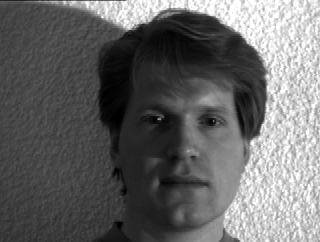
\includegraphics[scale=0.35]{Iluminacion1}
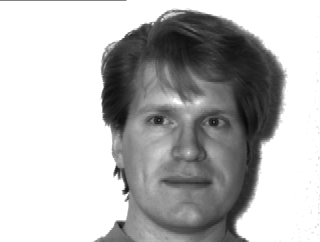
\includegraphics[scale=0.35]{Iluminacion2}
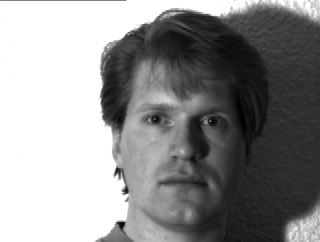
\includegraphics[scale=0.35]{Iluminacion3}
\caption{Ejemplos de la variación de la iluminación en un rostro. Extraídos de la base de datos "Yale A".}
\label{im:EjemIluminacion}
\end{figure}
\item \textit{Variación según el punto de visión}  \cite{hill1997information}.- El rostro es un objeto tridimensional y debido al ángulo de visión de la cámara la apariencia del rostro puede variar debido a la deformación proyectiva, la cual lleva a que la parte inferior de rostro se vea más angosta de lo que realmente es. Esto también se aplica para las rotaciones del rostro como se puede ver en la Figura \ref{im:EjemViewPoint}
\begin{figure}[h]
\center
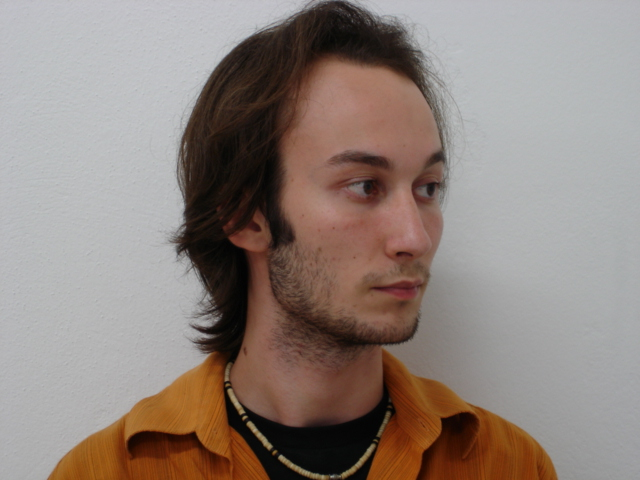
\includegraphics[scale=0.20]{ViewPoint1}
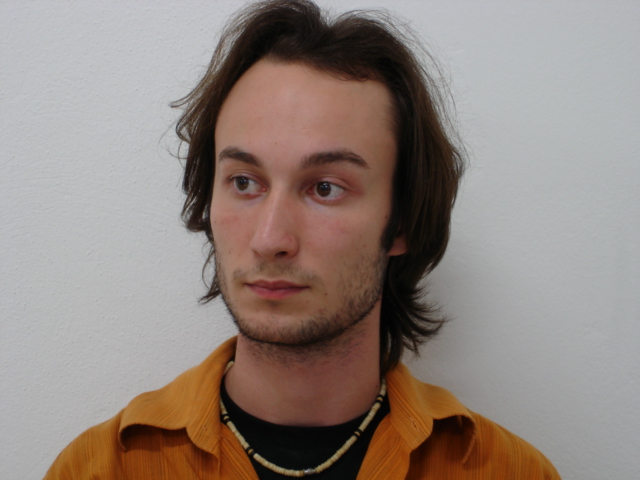
\includegraphics[scale=0.20]{ViewPoint2}
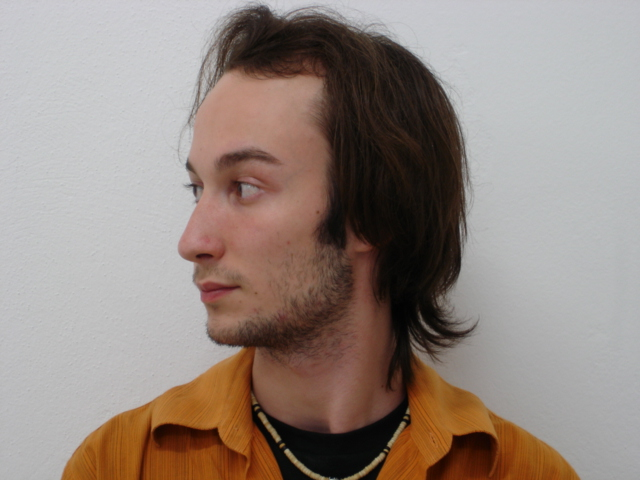
\includegraphics[scale=0.20]{ViewPoint3}
\caption{Ejemplos de como el punto de visión modifica un rostro. Extraídos de la base de datos "FEI".}
\label{im:EjemViewPoint}
\end{figure}
\item \textit{Expresión}.-  El rostro es un objeto no rígido, la expresión de la emociones es parte de la comunicación paralingüistica junto con el habla, y la variación de esas expresiones faciales influye en el reconocimiento del rostro. Ejemplos de ello se puede ver en la Figura \ref{im:EjemExpresion}
\begin{figure}[h]
\center
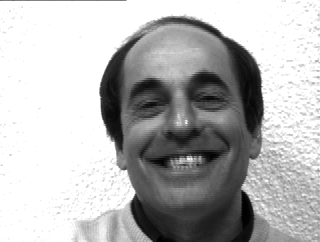
\includegraphics[scale=0.35]{Expresion1}
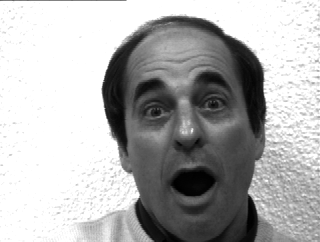
\includegraphics[scale=0.35]{Expresion2}
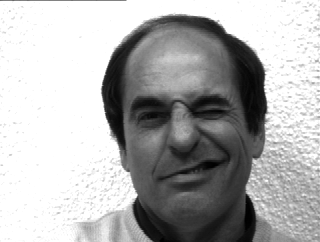
\includegraphics[scale=0.35]{Expresion3}
\caption{Ejemplos de la variación de la expresión en un rostro. Extraídos de la base de datos "Yale A".}
\label{im:EjemExpresion}
\end{figure}
\item \textit{Time delay}.- Es el intervalo de tiempo entre la adquisición de la imagen que se desea reconocer y la imagen o los datos con los cuales realizamos la identificación. Por ejemplo, intentar identificar a un sujeto el cual su ultima fotografía fue tomada hace un año.
\begin{figure}[h]
\center
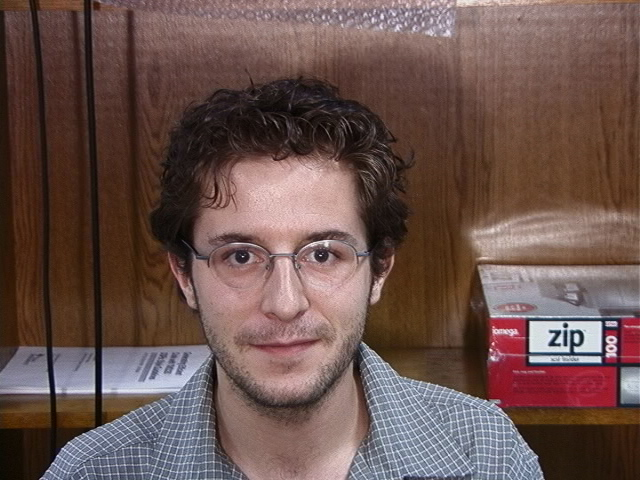
\includegraphics[scale=0.20]{Time1}
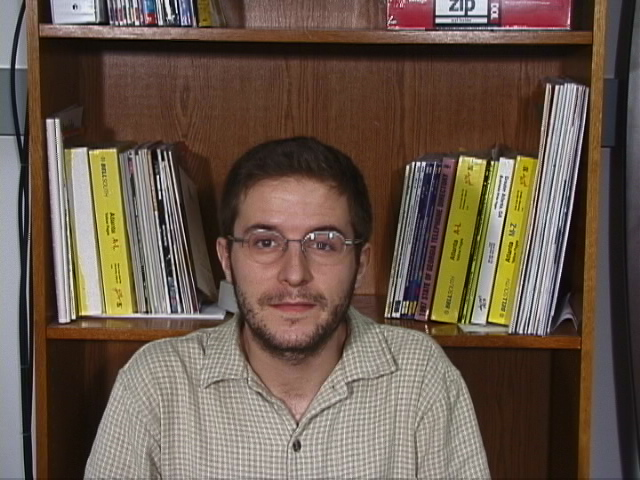
\includegraphics[scale=0.20]{Time2}
\caption{Ejemplos de la variación del tiempo en un mismo sujeto. Extraídos del la base de datos "Georgia".}
\label{im:EjemTimeDelay}
\end{figure}
\item \textit{Factores individuales}.- Se considera factores individuales a aquellos como el uso de maquillaje, estilos de peinado, disfraces, y otras formas en las que las personas modifican su apariencia a gusto personal. Un ejemplo de ello es el proyecto de ``CV Dazzle'' \cite{harvey2014cv} que usa el maquillaje para burlar las técnicas de detección de rostros como se puede ver en la Figura \ref{im:EjemMakeUp}.
\begin{figure}[h]
\center
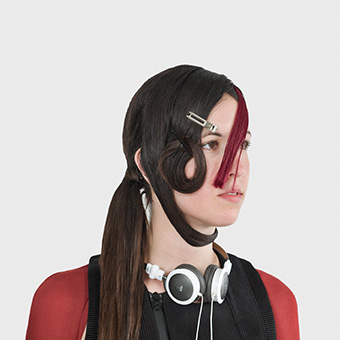
\includegraphics[scale=0.35]{MakeUp1}
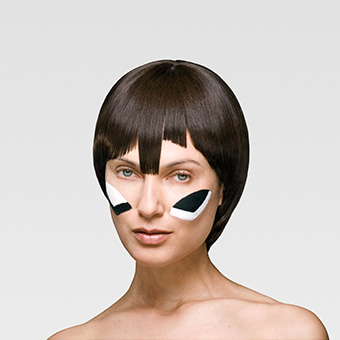
\includegraphics[scale=0.35]{MakeUp2}
\caption{Ejemplos extraídos del proyecto de ``CV Dazzle'' \cite{harvey2014cv}.}
\label{im:EjemMakeUp}
\end{figure}
\item \textit{Oclusión}.- La oclusión puede darse debido a objetos en la escena o al uso de lentes de sol y otros objetos, también debido a la falta de cooperación de los individuos y a la variación según el punto de visión, Figura \ref{im:EjemOclusion}.
\begin{figure}[h]
\center
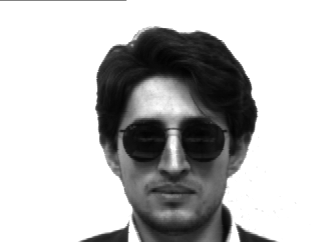
\includegraphics[scale=0.35]{Oclusion1}
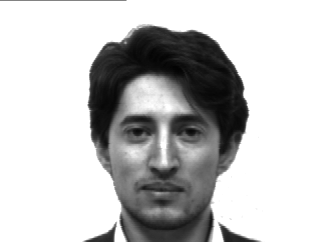
\includegraphics[scale=0.35]{Oclusion2}
\caption{Un ejemplo clásico de la oclusión del rostro es el uso de lentes de sol. Extraídos de la base de datos "Yale A".}
\label{im:EjemOclusion}
\end{figure}
\end{enumerate}

%Problemas de video vigilancia
A parte de los problemas listados, cuando el reconocimiento de rostros se aplica a  vídeo vigilancia surgen nuevas dificultades siendo las mas importantes:

\begin{enumerate}
\item \textit{La calidad del video}.- Debido a que la grabación de vídeo ocurre en ambientes no controlados todos los problemas anteriormente citados se presentan varias veces afectando la calidad final del vídeo. Cabe mencionar que a pesar de las mejora en resolución en las cámaras de vídeo vigilancia, frecuentemente se opta por equipos de gama baja en hogares y oficinas más como medida de disuasión que con el propósito de hacer vídeo vigilancia.
\item \textit{Falta de cooperación de los individuos}.- Es un problema que solo se presenta en vídeo vigilancia, debido a que en otros escenarios de reconocimiento de rostros como los presentados en la Tabla \ref{TaAplicaciones} siempre se puede esperar que las personas cooperen para ser identificas. Esto resulta ser uno de los motivos por el cual el reconocimiento de rostros es un problema de difícil resolución.
\item \textit{Las imágenes de los  rostros son pequeños}.- Debido a las condiciones de adquisición, las imágenes de los rostro son más pequeñas y de menor calidad de lo que asumen la mayoría de los sistemas de reconocimiento de rostros existentes. Por ejemplo, una región de rostros valida puede ser tan pequeña como 20$\times$20 pixeles, mientras los tamaños de las imágenes de los rostros usados en los sistemas actuales son tan grandes como 128$\times$128. El pequeño tamaño no solo hace la tarea de reconocimiento difícil, también afecta la precisión de la detección de puntos de interés que a menudo son necesarios en los métodos de reconocimiento.
\item \textit{Las características de los rostros como objetos} \cite{zhao2003face}.- El rostro humano como objeto es más fácil de reconocer si se compara con otro objeto que no sea un rostro (diferencia Inter-clase) pero resulta mas difícil de reconocer si se le compara con otro rostro (diferencia Intra-clase) por ello detectar y localizar rostros es más fácil que reconocer un rostro en especifico. 
\end{enumerate}

%conclusion sobre seccion // mencionar biometria
Como se ha podido observar en esta sección el reconocimiento de rostros en vídeo vigilancia es una tarea muy difícil debido a la conjunción de varios factores, como el ambiente no controlado donde aparecen todas las dificultades relacionadas al típico reconocimiento de rostros. A ello se suma los problemas del escenario de video vigilancia en el cual se puede esperar la falta de cooperación de los sujetos a identificar y finalmente la calidad de los videos y las imágenes de los rostros.

Como parte de la propuesta expuesta en detalle en el Capítulo \ref{chap:Propuesta} intentamos resolver el problema de reconocimiento de rostros en un \textit{pipeline} de video vigilancia bajo las condiciones de una cámara de seguridad en alta definición, proponemos enfrentar las variaciones de iluminación a través de técnicas de pre-procesamiento, afrontar en parte el problema de variación de poses con el uso de los últimos avances en el \acf{CLNF} y \acf{EBGM} como método de reconocimiento biométrico. 

\section{Objetivos}\label{scc:Objetivos}

\subsection{Objetivo general}
Proponer un \textit{pipeline} para el reconocimiento de rostros en una escena de vídeo con la adaptación de \acf{CLNF} y \acf{EBGM} para su uso final en vídeo vigilancia.

\subsection{Objetivos específicos}
Como objetivos específicos se tiene:
\begin{itemize}
\item Comparar los diferentes métodos holísticos existentes contra \ac{EBGM}.
\item Analizar el impacto de la modificación de parámetros de \ac{EBGM}.
\item Analizar la influencia de incrementar el conjunto de entrenamiento mediante transformaciones de perspectiva en \ac{EBGM}.
\item Desarrollar los métodos de mejora del \textit{pipeline} propuesto con \ac{EBGM}.
\item Probar el \textit{pipeline} propuesto en imágenes de vídeo vigilancia.
%\item Verificar el efecto que tiene el uso de \ac{CLNF} como opción al método de localización de puntos fiduciales de \ac{EBGM}.
\end{itemize}

\section{Alcance y limites de la tesis}
A partir de los problemas mencionados en la Sección \ref{ssc:PlanteamientoProblema} la propuesta, explicada en el Capítulo \ref{chap:Propuesta} enfrenta los siguientes problemas:
\begin{itemize}
 \item Iluminación.- Con el uso del pre-procesamiento explicado en las Sección \ref{scc:PropIluminacion} que permite iluminar u oscurecer imágenes según  la situación lo requiera, de esta manera lograr una normalización el lo referente a iluminación cuando existe luz diurna.
 \item Variación según el punto de visión, Expresión facial.- Estos dos problemas son enfrentados con el uso de \ac{CLNF} como detector de puntos ya que como se muestra en el Capítulo \ref{chap:Resultados} mejora el rendimiento del reconocimiento. debido a su mayor exactitud en encontrar puntos fiduciales independientemente de las expresiones faciales.
\item Falta de cooperación de los individuos.- Es enfrentado mediante la unión del detector de Viola-Jones, detector de \ac{HOG}. También entra en consideración la posición de la cámara que fue puesta de formal tal que pueda captar los rostros de los transeúntes, Figura \ref{im:EscenaViola}.
\end{itemize}

Problemas como baja calidad del vídeo, imágenes de rostros muy pequeñas no son enfrentados con la propuesta, mas allá del pre-procesamiento y transformación de tamaña propio de \ac{EBGM} ya que no se emplea ninguna técnica de súper-resolutorio o mejora de imagen. Para el caso de oclusión y factores individuales no se propone ninguna mejora al funcionamiento de los detectores usados mas que su combinación para validar rostros y tampoco se prueba la propuesta cuando las imágenes de vídeo vigilancia  son de tomas de luz infrarroja.

\section{Organización de la tesis}
En los próximos capítulos se desarrollará el trabajo que comprende toda la tesis, en esta sección se realiza una breve descripción de cada uno de ellos.

\begin{enumerate}
\item En el Capítulo \ref{chap:Revision} se desarrolla una explicación del reconocimiento de rostros, una categorización de los métodos de reconocimiento de rostros, establecemos las diferencias entre métodos basados en características y métodos holísticos, donde se presenta el estado del arte en el reconocimiento de rostros.

\item En el Capítulo \ref{chap:Conceptos} se expone el marco teórico de nuestra propuesta. 
Se realiza una introducción a las técnicas de reconocimiento probadas en esta tesis, se profundiza el funcionamiento de \ac{EBGM} y se explica las razones de su uso para este trabajo. Definimos el concepto de biométria y cuales son los requerimientos para que un método de reconocimiento sea considerado biométrico.

\item En el Capítulo \ref{chap:Propuesta} se describe en detalle la propuesta de esta tesis, concentrándose en el \textit{pipeline} de vídeo desde la detección de rostros hasta el resultados del reconocimiento.

Se menciona el aporte de la modificación de \ac{EBGM} usando \ac{CLNF} para su adaptación al uso de vídeo vigilancia, junto al uso de mejoras en la iluminación.

\item En el Capítulo \ref{chap:Resultados} se muestran los resultados experimentales de la propuesta junto con las opciones exploradas para lograr el objetivo del trabajo de tesis.

\item Finalmente en el Capítulo \ref{chap:Conclusiones} se mencionan las conclusiones obtenidas en esta tesis y se listan los posibles trabajos futuros en continuación a este trabajo.
\end{enumerate}

Se ha expuesto el contexto y la necesidad de contar con propuestas par afrontar el trabajo de vídeo vigilancia en este trabajo, es necesario seguir resaltando su dificultad no solo para los algoritmos de visión computacional, sino para la personas en diversas situaciones. %Inserta el capítulo 1 Introduccion
\chapter{Revisión Bibliográfica} \label{chap:Revision}
El reconocimiento de individuos usando el rostros se realiza a partir de imágenes, las cuales pueden ser estáticas (fotografías) o dinámicas (imágenes de vídeo). En el caso de la vídeo vigilancia se toma en cuenta el hecho que no se tiene control sobre varios factores que influye en proceso de reconocimiento como se explica en la sección \ref{ssc:PlanteamientoProblema}.

Según \textit{surveys} de la literatura como \cite{zhao2003face}, \cite{parmar2014face} y \cite{pandya2013survey} los métodos de reconocimiento de rostros se pueden categorizarse mediante el enfoque en por el cual abordan el problema, es decir como tratan a la imagen del rostro. En la figura \ref{im:metodos} se puede ver algunos algoritmos clasificados por enfoque. Siendo algunos de los más conocidos \acf{LDA} \citep{zhao1999subspace}, \acf{PCA} \citep{turk1991eigenfaces}, \acf{EBGM} (\cite{wiskott1997face}). % \cite{zhao2003face}.
\begin{figure}[h]
\center
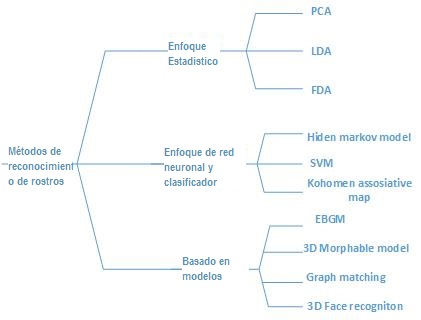
\includegraphics[scale=1]{Metodos}
\caption{Clasificación de métodos de reconocimiento de rostro por enfoque según \cite{zhao2003face}.}
\label{im:metodos}
\end{figure}

Como se observa en la Figura \ref{im:metodos} los métodos de reconocimiento de rostros pueden ser agrupados en métodos holísticos y métodos basados en características como en  \cite{tseng2003comparison} , y según \cite{zhao2003face} podemos agregar los métodos basados en inteligencia artificial y clasificadores o según \cite{parmar2014face} y \cite{pandya2013survey} pueden agregarse los métodos híbridos, pero las dos primeras clasificaciones son una constate en la literatura.

Los métodos holísticos tratan a la imagen como un todo, donde la extracción de características depende de la variación total de la información que conforma la imagen, por esta razón no sabemos que características se extraen, ni podemos darles una jerarquía de valores, esta es la razón por la cual son sensibles a cambios de iluminación y fondo. 

Este es el motivo por el cual varias de las contribuciones en estado del arte se concentran en presentar métodos holísticos robustos a esta clase de problemas como \cite{zhao1999theoretical} o nuevas forma de pre-procesamiento como \cite{gross2003image}.

Los métodos basados en modelos, también conocidos como basados en características, como lo dice su nombre se basan en formas localizadas de extracción de características o áreas localizadas de la imagen como pueden ser los ojos.
Generalmente el reconocimiento se realiza mediante una formula de distancia entre las características de dos diferentes imágenes, un buen ejemplo de ello es \ac{EBGM} en \cite{wiskott1997face} y en \cite{bolme2003elastic}.

Además \cite{zhao2003face} considera que se puede agregar a estas dos categorías un tercer enfoque basado en redes neuronal y clasificadores donde en vez de tener un formula de distancia, el reconocimiento se realiza a través de un clasificador o otro método basado en inteligencia artificial. Pero la extracción de características sigue dependiendo de una forma que puede encajar como método holístico o basado en características.

%Debido a ello para este trabajo de tesis se considera la separación de \cite{tseng2003comparison} y se usará como referencia para futuras comparaciones.
\section{Métodos holísticos}
En esta sección se hace una breve introducción a los métodos holísticos que se usan como referencia para la propuesta. Se menciona su funcionamiento general y sus principales características.


\subsection{\acf{PCA}}
\ac{PCA} es un método para la reducción de la dimensionalidad sin supervisión que puede ser aplicada para abordar el problema de reconocimiento de rostros. En \cite{sirovich1987low} se argumenta que cualquier imagen de rostro puede ser aproximadamente reconstruida como la suma con pesos de una pequeña colección de imágenes base que llaman \textit{eigenimages} y la media de las imágenes del rostro. Con ello \cite{turk1991eigenfaces} presenta su conocido método de \textit{eigenfaces}.

% A continuación una breve explica como funciona este método:

% Se supone que $\Gamma$ es un vector $N^2\times 1$ que corresponde a una imagen de rostro $N\times N$ llamada $I$ donde el objetivo es representar $\Gamma (\Phi-media)$ en un espacio de baja dimensión; $\Phi- media=w_1u_1+w_2u_2+.....w_ku_k$ donde $k<<N^2$ , $w$ es el peso asociado al \textit{eigenface} $u$.

% Entonces si se tiene un conjunto de imágenes de rostro del mismo tamaño ${I_1,I_2,...,I_Q}$ donde cada $I_i$ se puede representar como un vector $\Gamma_i$, se tiene que calcular el vector promedio de rostro $\Psi$:
% \[\Psi =\frac{1}{Q}\sum^Q_{i=1}\Gamma_i\] 
% La nueva representación del rostro es: 
% \[\Phi_i=\Gamma_i-\Psi\]
% Después se calcula una matriz de covarianza $Co$:
% \[Co=\frac{1}{Q}\sum^M_{n=1}\Phi_n \Phi^T_n=AA^T \]
% Siendo una matriz $N^2\times N^2$ donde $A=[\Phi_1\Phi_2...\Phi_M]$ es una matriz $N^2\times Q$.

% Sobre la matriz $AA^T$ se debe hallar auto vectores $u_i$, pero resulta ser una matriz muy grande lo que resulta poco practico, por lo que se considera la matriz $A^TA$ que es una matriz $Q\times Q$ donde si podemos calcula auto vectores $v_i$ siendo: 
% \[A^TAv_i=\mu_iv_i\]
% Dónde existe una relación de correspondencia donde los $Q$ autovalores y autovectores de $A^TA$ son los $Q$ autovalores y autovectores más grandes de $AA^T$. De esta manera mantenemos los $K$ vectores mas significativos. Ahora cada rostros esta representado por: 
% \[\Phi_i-media= \sum^{K}_{j=1} w_j u_j, (W_j=u^T_j\Phi_i)\]
% Dónde $u_j$ es un \textit{eigenface}, finalmente cada rostros puede ser representado como una colección de pesos:
% \[\Omega_i=\begin{bmatrix}
% w^i_1\\ 
% w^i_2\\ 
% ...\\ 
% w^i_k
% \end{bmatrix} , i=1,2,...,Q\]

% De esta manera \ac{PCA} reduce la dimensión de una imagen de rostro a un conjunto de pesos. 
Un problema que \ac{PCA} tiene, está relacionado al proceso de reducción en si donde no se sabe que características se están extrayendo y presenta una susceptibilidad a la variación de la data ingresada.

\subsection{\ac{KFA}}
\ac{KFA} \citep{liu2006capitalize} es un método que capitaliza la técnicas de incremento de la dimensionalidad, donde argumenta que métodos de reducción de dimensionalidad como \ac{PCA} tienen problemas reconociendo patrones complejos como lo es el rostro, por lo tanto es necesario un método que pueda reconocer patrones de alta dimensionalidad.

\ac{KFA} primero realiza un mapeo del espacio de la información de entrada a un espacio de características de alta dimensionalidad, y después implementa el análisis multiclase de Fisher en dicho espacio de características. \ac{KFA} usa Gabor Wavelets (en la sección \ref{scc::EBGM} se explica con más detalle) como método para incrementar la dimensionalidad.

\ac{KFA} posee varias ventajas sobre \ac{PCA} ya que su representación de la información permite una mejor distinción entre las clases que componen su espacio dimensional.

%\subsubsection{\ac{KPCA}}
%Es una forma no lineal de \ac{PCA} \cite{scholkopf1998nonlinear}, con el uso de una función integral como operador de una función Kernel, se pude computar con mayor eficiencia los componentes principales en un espacio de características. Su objetivo es presentar una forma de abordar el problema del calculo de auto valores que es necesario para poder realizar el proceso de \ac{PCA}.
%
%Obtiene ventajas sobre el típico \ac{PCA} porque puede reconocer patrones no lineales y la capacidad de adicionarle un kernel hace mas versátil a este método. Aunque \cite{scholkopf1998nonlinear} menciona que \ac{KPCA} no has ido comparado con otros métodos que analizan la información de forma no lineal.

\subsection{\acf{LDA}}
En aplicaciones aplicaciones típicas de reconocimiento de rostros tenemos vectores de imágenes de rostros de enormes dimensiones, y a pesar de ser proyectados en un sub-espacio, la dimensión de las características en varios casos son mayores a centenar, tampoco es conveniente que la dimensión del sub-espacio sea pequeña. %Este problema lleva a lo que se conoce como el fenómeno llamado \textit{dimensionality curse} que se refiere a los problemas se presentan al organizar y analizar data de alta dimensionalidad.

\ac{LDA} usado para el reconocimiento de rostros \citep{zhao1999subspace} es un método holístico que consiste en dos pasos: primero se proyecta la imagen del rostro de su representación original como vector a un sub-espacio de rostro a través de \ac{PCA}, luego usamos LDA para obtener un clasificador lineal en el sub-espacio de rostros creado. El criterio que se usa para determinar la dimensión del sub-espacio permite generar características que separan las clases a través de \ac{LDA} del total de la representación del sub-espacio.

\ac{LDA} presenta problemas relacionados a \ac{PCA} como poca tolerancia al ruido y su se obtiene datos de entrada con grandes variaciones de iluminación.

%parrafo de conclusion de seccion

En esta sección se ha descrito ejemplos de métodos holísticos de diferentes clases. Cada uno enfrenta el reconocimiento de rostros de manera diferente mediante reducción de dimensionalidad lineal, con un clasificador y con un aumento de la dimensionalidad. 

En todos ellos no sabemos que características estamos midiendo, en contraste con la próxima sección donde presentamos un método basado en características.

\section{Basados en modelos y características}
Un enfoque para abordar el reconocimiento de rostros es mediante el uso de modelos para poder hallar características locales las cuales son pueden se ponderadas para hallar una respuesta al reconocimiento de rostros. A continuación mencionamos:

\subsection{\ac{RFG}}
A diferencia de otros métodos donde se hace una comparación directa entre grafos, \ac{RFG} \citep{kafai2014reference} usa un conjunto de varios rostros en diferentes poses para crear un grupo de referencia(conjunto base) y así hacer una comparación indirecta a través del este conjunto base para ello hace uso de \ac{DCT} para medir la similaridad entre rostros.
A cada imagen del conjunto base se divide entre una malla de 2, 9, 16 hasta llegar a 100 secciones y a cada sección se le aplica una \ac{DCT} para crear un vector de características cada vector de representa a una persona del conjunto base en todas sus pose, y este vector es representado como un nodo en un grafo donde se relaciona con los demás rostros del conjunto base, cualquier nuevo rostro es comparado con este grafo de rostro en función a su similaridad y cercanía a los nodos, para así poder hallar su lugar en el grafo de esta manera los rostros a reconocer se miden en función al grafo de referencia

\subsection{\textit{Face recognition based on multiple facial features}}
Es un método similar al trabajo original de Wiskott \citep{wiskott1997face} donde también se usa un grafo que representa el rostro donde cada nodo representa un punto de interés el cual contiene un vector de características generado a través de convoluciones usando Gabor wavelet, este método se diferencia por usar solo 17 puntos de interés un una medida de similaridad propuesta como \textit{Two-Layer Nearest Neighbor} \cite{liao2000face} que busca cual similar los cada nodos del grafo con sus respectivas contra partes en los grafos de los rostros a reconocer la similaridad final se calcula como la división de la sumatoria de todos los nodo por los $H$ nodos mas importantes donde el valor de $H$ es definido como 5 por el autor.

\subsection{Local Graph Matching}
En lugar de usar un solo grafo como EBGM, Local Graph Matching \citep{fazl2007robust} usa un conjunto de grafos de 3 nodos y 3 aristas donde cada nodo es un punto distintivo en la imagen del rostro. para calcular los puntos de interés se calcula en una fase de entrenamiento el rostro medio donde se distinguen los punto con mayor variación estadística, a partir de los puntos encontrados se generan grafos triangulando los puntos que estén mas próximos entre si.
Para su fase de reconocimiento se utiliza una convolución con un Gabor wavelet para extraer características y se utiliza similaridad de cosenos para calcular a quien pertenece la imagen a reconocer.

\subsection{3-D Morphable Model}
3-D \textit{Morphable Model} se utilizan para el análisis de rostros debido a las propiedades intrínsecas de los rostros en 3D que proporcionan una representación que es inmune a las variaciones intra-personales como la pose y la iluminación. 

En \cite{huang2003component} dada una imagen de entrada facial individual, un 3-D \textit{Morphable Model} puede recuperar el rostro en 3D (forma y textura) y propiedades de la escena (pose y la iluminación) a través de un proceso de adaptación. El proceso de reconocimiento se realiza mediante una comparación de características con el modelo 3D puesto en la misma posición que la imagen a identificar.


%\subsection{\acf{EBGM}}
%\ac{EBGM}  es un algoritmo de inspiración biológica para el reconocimiento de objetos en el campo de la visión computacional. Se apoya en el argumento que las características visuales utilizadas basadas en Gabor Wavelet, han probado ser un buen modelo del procesamiento visual temprano en el cerebro, más precisamente células simples en la corteza visual primaria. 

%Los objetos visuales en \ac{EBGM} se representan como grafos etiquetados, donde los nodos representan texturas locales basados en Gabor Wavelet. Así, una imagen de un objeto se representa como una colección de texturas locales en una determinada disposición espacial. 

%El reconocimiento se realiza a partir de comparaciones entre grafos para medir su parecido. Este método de reconocimiento es ampliado en la sección \ref{scc::EBGM}.

\section{Basados en redes neuronales}

La idea básica del uso de una red neuronal es adaptar la red con una entrada para cada pixel, pero como esto es una solución poco practica debido a la gran cantidad de pixeles, una solución es modificar los datos de entrada de la red a través de alguna técnica de reducción de dimensionalidad o algún método de extracción de características.

Una propuesta del uso de redes neuronales es \cite{cottrell1990face}  donde se utiliza dos redes perceptron multicapa con \textit{back propagration} donde la primera capa trabaja en modo auto asociado extrayendo características para la segunda capa donde se realiza la clasificación. Es propuesto como un método para reconocer una gran cantidad de imágenes pero el autor menciona que inclusive en buenas condiciones no mejora el desempeño en comparación a \ac{PCA}.

Otro método de reconocimiento de rostros automatizado es presentado por \cite{lin1997face}, donde utiliza una red neuronal que se basa en la toma de decisiones probabilísticas \ac{PDBNN}, consta de tres módulos, detector de rostros, detector de ojos, y reconocedor de rostros. Este método se diferencia de otros porque utiliza la zona de la cara que contiene las cejas los ojos y la nariz, pero no la boca. La boca no se considera por que presenta muchas variaciones por el cambio de expresión facial, por lo que al fin de lograr un método robusto a cambios de expresión se descarto esa zona.

Las \acf{PDBNN} tienen una característica única, que es su estructura modular. Es decir, para que se reconozca cada clase, el \ac{PDBNN} dedica una de sus sub-redes para la representación de esta clase. En comparación con la mayoría de los sistemas de reconocimiento multi-clase utilizando una función de discriminar entre dos clases, tiene \ac{PDBNN} una menor tasa de falsas alarmas-rechazo debido a que sus funciones discriminantes obedecen a una restricción probabilística.

En \cite{er2002face} se  presentó un método holístico para el reconocimiento facial, donde las características se extraen con \ac{PCA} y se utilizan como entrada para una red neuronal \ac{RBF}. Las redes \ac{RBF} tienen un buen rendimiento para los problemas de reconocimiento, tienen topología compacta y el aprendizaje es rápido. Además de las tareas de reconocimiento de rostro tradicionales  (identificación y verificación de la identidad) las redes neuronales se han utilizado para diversas tareas, tales como la identificación de género y el reconocimiento de expresiones faciales. 

\section{Consideraciones finales}
El reconocimiento de rostros es un área con una gran cantidad de trabajos y muy amplia en técnicas como se vio en este capitulo, cabe resaltar las varias formas en que la totalidad de técnicas presentadas en el estado del arte pueden ser agrupadas, ya que no existe un consenso unificado en su clasificación.

En el estado del arte aun son pocas las propuesta de llevar el reconocimiento de rostros a la vídeo vigilancia como se observa en el Capitulo \ref{chap:Intro} por ello su necesidad de proponer y probar propuestas para lograr un reconocimiento de rostros en vídeo vigilancia abordando todas las dificultades que se presenta en este tipo de escenarios donde el ambiente no es controlado.


\chapter{Marco teórico de la propuesta}\label{chap:Conceptos}
En este capítulo se presenta todos los conceptos y técnicas usadas para el desarrollo de la propuesta desde las técnicas de detección usadas hasta el proceso de reconocimiento.

\section{Métodos de detección}

Es necesario resaltar la importancia de una detección adecuada para el reconocimiento ya que ambos son procesos muy relacionados entre sí. En esta sección se explican tres métodos de detección uno para encontrar rostros, otro para validar los rostros detectados y finalmente uno para encontrar puntos de dentro de los rostros.


\subsection{Detector de Viola-Jones}\label{scc:Viola}
El detector de Viola-Jones también conocido como \textit{Haar Detector} en implementaciones libres, se presenta en \cite{viola2001rapid} donde se hace uso de las características Haar (Figura \ref{im:Haar}) en una representación conocida como Imagen Integral, también se utiliza el Algoritmo Ada Boost y un clasificador en casada para completar el proceso de detección.

\begin{figure}[h]
\center
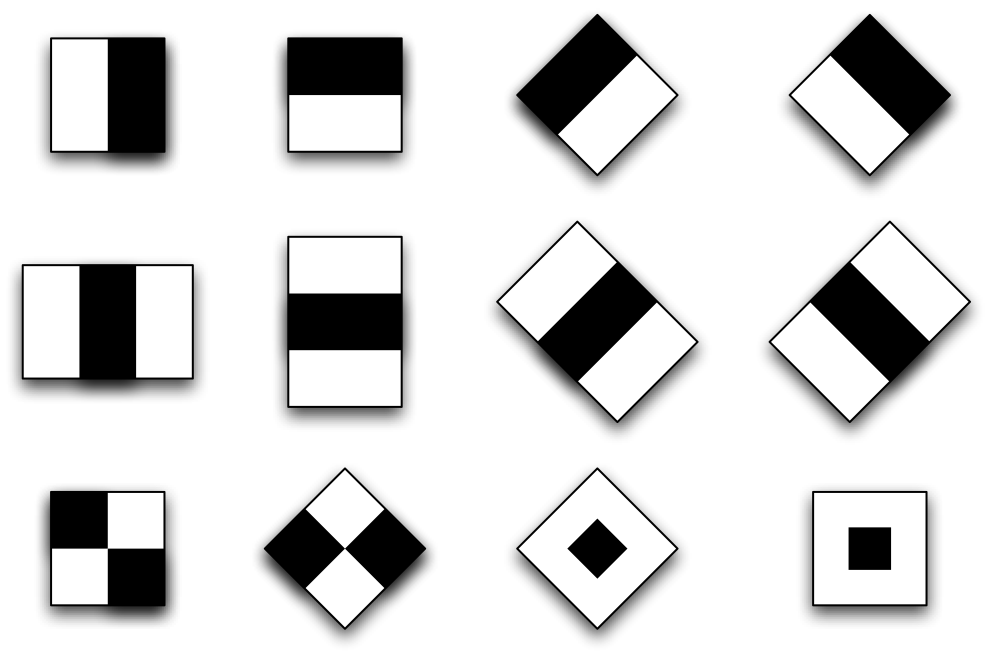
\includegraphics[scale=.5]{Haar}
\caption{Ejemplo de característica Haar, extraído de \cite{viola2001rapid}. Estos rectángulos pueden ser entendidos como rectángulos en los cuales son determinados como áreas de baja iluminación y otros como áreas de alta iluminación de esta manera podemos representar el contraste entre dos secciones de la imagen,}
\label{im:Haar}
\end{figure}

En \cite{viola2001rapid} se explica que el trabajo de detección se basa en tres conceptos:
\subsubsection{Imagen integral}
Usa un concepto parecido a una tabla de texturas donde tenemos en cada punto el valor de la suma de los pixeles de arriba y a la derecha de dicho punto. 

Esto permite el calculo rápido de valor de los pixeles para cualquier sección de la imagen, dicho valor nos ayuda a hacer un calculo rápido del contraste en cualquier sección, lo cual permite el calculo de cualquier característica Haar en tiempo constante.
\subsubsection{Algoritmo Ada Boost}
Debido a la existencia de un gran numero de características Haar, aproximadamente más de 45,000 no es posible usar todas en un proceso de clasificación, por lo que es necesario encontrar un conjunto pequeño de características que juntas formen un clasificador efectivo.

En \cite{viola2001rapid} se presenta una modificación al algoritmo Ada Boost para seleccionar las mejores características Haar y con ellas entrenar varios clasificadores débiles en términos de su tasa de aciertos, que en combinación permiten obtener un clasificador fuerte. De esta manera tener un clasificado robusto para el proceso de detección.
\subsubsection{Clasificador en casada}
La idea tras un clasificador en cascada es organizar todos los clasificadores débiles en un estilo en el cual estén uno detrás de otro como una cascada. Cuando se analiza una región esta pasa por el primer clasificador y sí el resultados es negativo se descarta, pero si resulta positivo pasa al siguiente clasificador hasta el final de la cascada y así sucesivamente de esta manera obtiene un solo clasificador, más robusto que los clasificadores que lo componen. Este proceso se puede apreciar en la Figura \ref{im:cascade}.

\begin{figure}[h]
\center
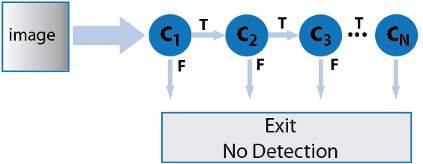
\includegraphics[scale=0.75]{cascadeClassifier}
\caption{Muestra del clasificador en cascada, donde una imagen es analizada por un clasificador tras otro desde el primero hasta el n-esimo si resulta la imagen positiva, extraído de \cite{viola2001rapid}.}
\label{im:cascade}
\end{figure}

El detector de Viola-Jones es ampliamente usado y reconocido como un detector que entrega una gran cantidad de verdaderos positivos (detecciones acertadas). Pero es necesario mencionar sus limitaciones y falencias, de la misma manera que entrega un gran porcentaje de verdaderos positivos también entrega falso  positivos (detecciones presentadas como verdaderas pero que no lo son) esto es debido a que el calculo de la imagen integral se hace en la escala de grises a veces alguna configuración de sombras producidas en la imagen genera la misma distribución de contrastes que un rostro humano.

Otro defecto es que solo detecta rostro de frente. No puede detectar otras posiciones del rostro humano simultáneamente. A pesar de estas deficiencia sigue siendo usado no solo para rostros sino para otro tipo de objetos ya que su mayor ventaja es que es entrenarle.

\subsection{Detector de \acf{HOG}}
Un detector de \acf{HOG} usa una combinación del descriptor de \ac{HOG} y un clasificador basado en \acf{SVM}, originalmente usado para detectar personas \cite{dalal2005histograms}, su uso se ha incrementado a varias situaciones, incluyendo la detección de rostros, a continuación exponemos las ideas detrás de este detector.
\subsubsection{Descriptor de \ac{HOG}}
Un descriptor de \ac{HOG} muestra el calculo de la gradiente de una imagen, la gradiente es cambio de la intensidad de la imagen en una cierta dirección, pudiendo ser representado como un vector que posee magnitud $g$ y dirección $\theta$, el calculo del gradiente en una imagen se hace por pixel y retorna la dirección del cambio y su magnitud, este proceso se observa en las siguientes ecuaciones:
\begin{equation}
dx=I(x+1,y)-I(x-1,y)
\end{equation}
\begin{equation}
dy=I(x,y+1)-I(x,y-1)
\end{equation}
\begin{equation}
\theta(x,y)=arctan\left(\frac{dy}{dx}\right)
\end{equation}
\begin{equation}
g(x,y)=\sqrt[2]{dx^2+dy^2}
\end{equation}

Donde $x$ y $y$ son las coordenadas de la imagen y la función $I(x,y)$ es el valor del pixel o intensidad en dichas coordenadas. Luego se divide la imagen en secciones iguales y en cada una de estas secciones se calcula un histograma de las orientaciones para conocer la orientación dominante de cada sección, de esta manera creamos un vector de características.

Con esta información se puede describir el contorno y forma de una figura, lo que es útil para realizar una clasificación.

\subsection{\acf{SVM}}
Un \ac{SVM} \cite{cortes1995support} es un clasificador lineal en el cual se intenta crear una linea divisoria entre las representación (vectores de características) de ejemplos positivos y negativos de un objeto determinado.

Esta basado en el aprendizaje estadístico para resolver problemas de clasificación de patrones. Los clasificadores lineales se caracterizan porque aprenden una función lineal para separar las clases. No se trata de una agrupación por similitudes, sin que existe una separación definida entre clases.

Dado un conjunto de ejemplos de entrenamiento (muestras) podemos etiquetar las clases y entrenar una SVM para construir un modelo que prediga la clase de una nueva muestra. Intuitivamente, una SVM es un modelo que representa a los puntos de muestra en el espacio, separando las clases por una linea representada por la función del clasificador. Cuando las nuevas muestras se ponen en correspondencia en función de su proximidad, pueden ser clasificadas a una u otra clase, dependiendo de la proximidad a cada una. Mas formalmente, la idea principal de SVM es construir un hiperplano o conjuntos de hiperplanos en un espacio de dimensionalidad muy alta como superficie de decisión, de tal forma que, el margen de separación entre ejemplos positivos y negativos sea el máximo. Una buena separación entre las clases permitirá una clasificación correcta. 

\ac{SVM} resulta ser un clasificador muy robusto y usado, el cual presenta varias modificaciones alrededor del estado del arte.


\subsection{\acf{CLNF}}
\ac{CLNF} es un método para encontrar puntos de interés en imágenes de rostros presentado en \cite{baltrusaitis2013constrained} e implementado para aplicaciones de video en \cite{Baltrusaitis2016} en la presentación de su framework ``Open Face'' para el tracking y detección de rostros, donde publica el código de su propuesta, \ac{CLNF} se basa en \ac{CLM}, por lo tanto empezamos con una explicación de \ac{CLM}.

\ac{CLM} es una forma para localizar un conjunto de puntos restringido por un modelo en una imagen, el proceso consiste en tomar una muestra de una área de la imagen donde se realizó una estimación inicial proyectarla a un marco de referencia. Por cada punto se genera una imagen de respuesta donde se le da una puntuación por tener el punto a localizar en cada pixel. Este puntaje es determinado a través de un detector local que evalúa el punto según un modelo de distribución de puntos en donde penaliza distribuciones complicadas y premia distribuciones simples y mas probables, de esta manera se evalúan todos los puntos en conjunto.

En \cite{baltrusaitis2013constrained} se propone el uso de redes neuronales para los detectores locales de los puntos, con lo cual logra una mejor determinación de puntos en relación con el resto de puntos detectados. Compara sus resultados con otras técnicas del estado del arte así mismo realiza pruebas con imágenes obtenidas de Internet que presentan condiciones no controladas.

\section{Técnicas de pre-procesamiento}
Como se puede observar en las secciones anteriores un problema en especial difícil es la iluminación, por lo que es necesario hablar sobre las técnicas de pre-procesamiento, se entiende como pre-procesamiento a las técnicas que modifican una imagen para acentuar alguna característica, estas serán usadas para afrontar dicho problema.

\subsection{Ecualización de histograma}
Las ecualización del histograma de una imagen es una transformación que pretende obtener para una imagen un histograma con una distribución uniforme. Es decir, que exista el mismo número de pixeles para cada nivel de gris del histograma de una imagen monocroma \cite{orlova2002image}.
La función de la ecualización es:
\begin{equation}
h(v)=Redondeo\Bigg(\frac{cdf(v)-cdf_{min}}{(M\times N)-cdf_{min}} \times (L-1)\Bigg)
\end{equation}
Donde $cdf_{min}$ es el mínimo valor no nulo de la función de distribución de acumulación. $M\times N$ es el numero de pixeles en la imagen y $L$ es el numero de niveles de la escala de gris.

\begin{figure}[h]
\center
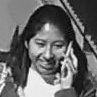
\includegraphics[scale=1]{face_original}
\hspace{1cm}
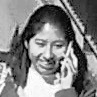
\includegraphics[scale=1]{face_he}
\caption{Ecualización de histograma - Izquierda: imagen en escala de Grises. Derecha: imagen ecualizada.}
\label{im:he}
\end{figure}


\subsection{Transformada de logaritmo}
La Transformada de logaritmo asigna un rango estrecho de valores (píxeles en escala de grises o un canal de un espacio de color) de un rango amplio de valores de entrada. La transformada de logaritmos es útil si se necesita expandir los valores de píxeles oscuros de una imagen mientras se comprime los valores altos \cite{thamiz2015liter}

\begin{equation}
\label{f_log}
s = c*log(1+ 256*r)
\end{equation}

Donde $r$ es la imagen de entrada, $c$ es una constante, $s$ es la imagen mejorada. Para la transformada de logaritmo se utilizo el valor de 20 para la constante $ c $. 

\begin{figure}[h]
\center
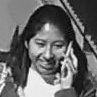
\includegraphics[scale=1]{face_original}
\hspace{1cm}
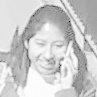
\includegraphics[scale=1]{face_log}
\caption{Transformada de logaritmo - Izquierda: imagen en escala de Grises. Derecha: imagen con Transformada de logaritmo.}
\label{im:log}
\end{figure}

\subsection{Transformada discreta de coseno}
La transformada Discreta de coseno (DCT por sus siglas en ingles) es utilizada especialmente en el procesamiento de señales e imágenes. DCT expresa en una secuencia finita de puntos, datos en términos de sumas de funciones de coseno en diferentes frecuencias. En el procesamiento de imágenes, la utilización de DCT ayuda a descomponer una imagen en frecuencias, donde usualmente los pequeños componentes de frecuencia altas pueden ser descartados. La ecuación en 2D está dada por la Ecuación. \ref{f_dct}
\cite{thamiz2015liter}\cite{vish2015ill}

\begin{equation}
	\label{f_dct}
	\resizebox{0.91\hsize}{!}{
		$ C(u,v) = \alpha(u)\alpha(v)\sum\limits_{x=0}^{N-1} \sum\limits_{y=0}^{N-1}f(x,y)cos\left[\frac{\pi(2x + 1)u}{2N}\right]cos\left[\frac{\pi(2y + 1)v}{2N}\right] $
	}
\end{equation}

Donde: $u$, $v$, $N$, $\alpha(u)$ y $\alpha(v)$ se definen de igual forma que la ecuación 1D. La ecuación inversa está definida por la Ecuación. \ref{f_idct}.

\begin{equation}
	\label{f_idct}
	\resizebox{0.91\hsize}{!}{
		$ f(x,y) = \sum\limits_{x=0}^{N-1}\sum\limits_{y=0}^{N-1} \alpha(u)\alpha(v)C(u,v)cos\left[\frac{\pi(2x + 1)u}{2N}\right]cos\left[\frac{\pi(2y + 1)v}{2N}\right]$
	}
\end{equation}

El resultado de la transformada de coseno, es una matriz de coeficientes positivos y negativos, los cuales representan la adición o resta de una determinada frecuencia para generar la imagen procesada por la transformada discreta de Coseno.

%parrafo para dar conclusion a la seccion
Se ha expuesto tres técnicas de pre-procesamiento que serán usadas en usadas en la propuesta del Capítulo \ref{chap:Propuesta}, todas abordan el problema de la iluminación de manera diferente, es necesario tener en cuenta que este problema ha sido tratado mucho en el estado del arte pero aun no se encuentra una técnica de mejora de iluminación sea robusta en cualquier escenario.

%En la siguiente sección se expone los métodos de detección usados como parte de nuestra propuesta. Se explica su funcionamiento y su posición en el estado del arte.


\section{\acf{EBGM}}\label{scc::EBGM}
%Después de haber tratado los métodos de pre-procesamiento, finalmente se expone las técnica de reconocimiento de rostro que en el Capítulo \ref{chap:Propuesta} se presenta una modificación.

\ac{EBGM} presentado en \cite{wiskott1997face} se basa en el concepto que las imágenes de los rostros reales tienen muchas características no lineales que no son abordadas por los métodos de reconocimiento holísticos, tales como variaciones en la iluminación, pose y expresión.
También se apoya en el argumento que las características visuales que se basan en Gabor Wavelet, han probado ser un buen modelo del procesamiento visual temprano en el cerebro, más precisamente células simples en la corteza visual primaria, por ello también se considera un algoritmo inspiración biológica.

Para ello, una transformación de Gabor wavelet crea una arquitectura de enlaces dinámicos que proyecta el rostro en una malla elástica que es conocida como Face Graph.
El Gabor Jet es un nodo en la malla elástica, el cual describe el comportamiento alrededor de un pixel. Esto es el resultado de la convolución de una imagen con varias máscaras de Gabor, el cual es usado para detectar formas y extraer características.

El reconocimiento esta basado en la similaridad de la respuesta mascara de Gabor a cada nodo. La dificultad con este método es el requerimiento de marcar puntos precisos en los rostros.

A continuación se explica en detalle su funcionamiento

\subsection{Gabor Wavelet}\label{sscc:GaborWavelet}
Las Gabor Wavelet son funciones que modifican las imágenes en el espacio de las frecuencias. El espacio de las frecuencia esta estrechamente relacionado al análisis de Fourier, por lo que es necesario hacer una breve descripción.

Una transformada de Fourier descompone una señal de tal manera que pueda ser representada como una combinación de sinusoidales. Cuando se procesa señales como lo pueden ser las imágenes, son representadas como una longitud de onda, ello es muy útil ya que revela información que no puede ser vista cuando observamos la imagen original.

Mientras una señal es un función en base al tiempo, la transformada de Fourier es una función en base a la frecuencia, se puede observar la transformada de Fourier en una dimensión en la siguiente ecuación:

\begin{equation}
F(x(t))(\omega)=\int_{-\infty }^{\infty } x(t)e^{-i\omega t}dt
\end{equation}

En la transformada de Fourier y en los Gabor Wavelet la función comprende una parte imaginaria y una real:

\begin{equation}
F(x(t))(\omega)=\int_{-\infty }^{\infty } x(t)cos(\omega t)dt - i\int_{-\infty }^{\infty } x(t)sen(\omega t)dt
\end{equation}

Cuando una transformada de Fourier se aplica una frecuencia en particular el resultado es un numero complejo que corresponde a la amplitud del coseno y del seno de la función original, en cada frecuencia hay un componte real y otro imaginario.

Las Gabor Wavelet son como la transformada de Fourier solo que tiene un alcance limitado, básicamente son una sinusoidal multiplicada por una Gaussiana.

Cuando una función es convolucionada con un Gabor Wavelet la información más cerca al centro de la campana de la Gaussiana es la que es tomada en cuenta mientras la más lejana es ignorada.

La ecuación de una de una Gabor Wavelet es la siguiente:
\begin{equation}
W(t,t_0,\omega)=e^{-\sigma(t-t_0)^2} e^{--i\omega(t-t_0)}
\end{equation}
y su convolucion es:
\begin{equation}
C(x(t))(t_0,\omega)=\int_{-\infty}^{\infty}x(t)W(t,t_0,\omega)dt
\end{equation}

De la misma manera que Fourier produce una resultado complejo un Gabor Wavelet produce:
\begin{equation}
C(x(t))(t_0,\omega)=a_{real}+ia_{imag}
\label{ec:ConvolucionWavelet}
\end{equation}

Mientras las ecuaciones presentadas hasta ahora trabajan en una dimensión es necesario presentar una forma en la que se pueda trabajar en dos dimensiones, esta es la representación del Gabor Wavelet como mascara para una convoluciónn en imágenes.

La Ecuación \ref{GaborWavelet} define como crear una máscara de Gabor donde $x, y$ son las posiciones en la mascara, para cualquier tamaño de mascara.
%El Gabor Jet es un nodo en la malla elástica, el cual describe el comportamiento alrededor de un pixel. Esto es el resultado de la convolución de un pixel de la imagen con varios Gabor wavelet o máscaras de Gabor, los cuales son usados para detectar formas y extraer características.

\begin{equation}
W(x,y,\theta,\lambda, \phi, \sigma, \gamma )=e^{-\frac{x'^2+\gamma y'^2}{2 \sigma^2}}cos(2\pi \frac{x'}{\lambda}+\phi) 
\label{GaborWavelet}
\end{equation}
\begin{equation*}
x'=cos\theta+ysin\theta   
\label{GaborWaveletx}
\end{equation*}
\begin{equation*}
y'=-x sin\theta+ycos\theta
\label{GaborWavelety}
\end{equation*}
Los parámetros usados para la construcción de los Gabor wavelet son los mismo que se utilizan en la implementación de \cite{bolme2003elastic}, a continuación los explicamos brevemente:
\begin{itemize}
\item $\theta$ especifica la orientación del Gabor Wavelet.\\
Siendo $\theta \in \left\{0,\pi/8,2\pi/8,3\pi/8,4\pi/8,5\pi/8,6\pi/8,7\pi/8 \right\}$
\item $\lambda$ especifica el ancho de onda de la función seno, empieza con 4 pixeles y aumenta en medias octavas siendo $\lambda \in \left\{4,4\sqrt{2},8,8\sqrt{2},16\right\} $
\item $\phi$ especifica la fase de la función seno, pudiendo ser par e impar que representa la parte imaginaria y la parte real del wavelet respectivamente.
Siendo $\left\{0,\pi/2\right\}$
\item $\delta$ especifica el radio de la Gaussiana. En este caso $\delta=\lambda$.
\item $\gamma$ especifica el ratio de aspecto de la Gaussiana. Este parámetro es incluido para que el Wavelet se aproxime a ciertos modelos biológicos. Siendo $\gamma=1$.
\end{itemize}


De esta manera podemos crear varios tamaños de máscaras que en la configuración original son $N \in \left\{25, 37, 51, 71, 101 \right\}$. Dando 80 configuraciones de Gabor wavelet y siendo efectivas 40 máscaras por punto, debido a que existe una mascara que extraer la parte imaginara y otra la parte real del Wavelet.
%buscar imagen de las mascaras

Al conjunto coeficientes (reales e imaginarios) producidos por estas mascaras de Gabor son llamados Gabor Jet que son el corazón de todo el proceso de reconocimiento de \ac{EBGM}.

A continuación se explica como es el proceso por el cual \ac{EBGM} determina en que puntos de una imagen va extraer características. A estos punto se les conocen como puntos fiduciales.

\subsection{Localización de puntos fiduciales}
Como se menciona en la sección anterior la convolución del conjunto de mascaras de Gabor sobre un punto produce un Gabor Jet que es un conjunto de coeficientes.

\begin{figure}[h]
\center
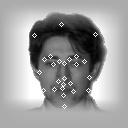
\includegraphics[scale=1.5]{Points}
\caption{Muestra de los puntos fiduciales elegidos en \ac{EBGM}\cite{bolme2003elastic}, en cada punto se realiza 40 convoluciones con máscaras de Gabor para crear un Gabor Jet por punto}
\label{im:puntos}
\end{figure}

Siguiendo el trabajo de \cite{wiskott1997face}, Bolme realiza una implementación de código libre de todo el algoritmo y da un mayor detalle de su funcionamiento, listando que puntos de interés debemos encontrar en una imagen. Estos puntos son conocidos como puntos fiduciales, en el Cuadro \ref{ta:PuntosFiduciales} se puede observar una lista de ellos, y en la Figura \ref{im:puntos} se puede ver su localización.

\begin{table}[h]
\centering
\caption{Lista de puntos fiduciales presentada en \cite{bolme2003elastic}}
\label{ta:PuntosFiduciales}
\begin{tabular}{|l|l|}
\hline
1. Ojo izquierdo                          & 2. Ojo derecho                          \\ \hline
3. Centro del puente de la nariz          & 4. Pico de la ceja izquierda            \\ \hline
5. Pico de la ceja derecha                & 6. Interior de la ceja izquierda        \\ \hline
7. Interior de la ceja derecha            & 8. Exterior de la ceja izquierda        \\ \hline
9. Exterior de la ceja derecha            & 10. Centro de la punta de la nariz      \\ \hline
11. Centro de la base de la nariz         & 12. Izquierda de la base de la nariz    \\ \hline
13. Derecha de la base de la nariz        & 14. Centro parte superior boca          \\ \hline
15. Centro parte inferior boca            & 16. Esquina izquierda de la boca        \\ \hline
17. Esquina derecha de la boca            & 18. Parte central del tope de la cabeza \\ \hline
19. Parte izquierda del tope de la cabeza & 20. Parte derecha del tope de la cabeza \\ \hline
21. Costado izquierdo del rostro          & 22. Costado derecho del rostro          \\ \hline
23. Centro de la barbilla                 & 24. Quijada izquierda                   \\ \hline
25. Quijada derecha                       &                                         \\ \hline
\end{tabular}
\end{table}

El método por el cual \ac{EBGM} encuentra los puntos fiduciales es a través del uso de moldes, imágenes en  las cuales los puntos han sido encontrados manualmente. En los trabajos de \cite{wiskott1997face} y \cite{bolme2003elastic} utilizan 70 imágenes normalizada a un mismo tamaño y donde las coordenadas de los ojos son las mismas.

Sobre cada imagen de molde y en cada punto marcado se realiza las convoluciones de las mascaras de Gabor para producir un Gabor Jet, de esta manera todos los puntos en todas las imágenes tienen un Gabor Jet. Finalmente todos los Gabor de un punto, por ejemplo el ojo izquierdo, son reunidos en un solo grafo conocido como Bucnh Graph que contiene todos los Gabor Jet de los modelos.

De esta manera se obtiene un modelo general con información de todos los modelos, también contiene la información de coordenada de cada punto en cada modelo y un punto de coordenada promedio.

Para reconocer una nueva imagen se realiza una normalización de tamaño y una traslación coordenadas de los ojos a coordenadas preestablecidas a través de una transformación matricial. Mediante un alineamiento entre las coordenadas normalizadas de los ojos y las coordenadas de los ojos del Bunch Graph se encuentran el resto de los puntos fiduciales en la imagen usando la información de coordenada promedio almacenada en el Bunch Graph. Finalmente se encuentra la posición final del punto usando como referencia el Gabor Jet con mayor similaridad en el Bunch Graph

Según \cite{bolme2003elastic} y \cite{wiskott1997face}, y como se menciona en la sección anterior el resultado de una transformada de Fourier en una función y en una frecuencia determinada es un numero complejo, que tiene una correspondencia en amplitud en términos de senos y cosenos que pueden ser representada como una coordenada polar.
\begin{equation}
x_{\omega}(t)=a_{\omega,r}cos(t)+a_{\omega,i}sin(t)= a cos(t+\phi).
\label{ec:CorrepondeciaAPolar}
\end{equation}
Es posible representar las suma de las sinusoidales como una función coseno dándole una amplitud y fase especifica.
Esto sucede cuando las sinusoidales son multiplicadas por una Gaussiana como se observa en la Ecuación \ref{ec:ConvolucionWavelet} y según lo visto en la Ecuación \ref{ec:CorrepondeciaAPolar} se puede representar los coeficientes complejos del resultado de las convoluciones como coordenadas polares de magnitud $a$ y un angulo $\phi$
\begin{equation}
a_{real} = a cos\phi 
\end{equation}
\begin{equation}
 a_{imag} = a sen\phi 
\end{equation}
y podemos halla $a$ y $\phi$ mediante:
\begin{equation}
a = \sqrt{a^2_{real}+a^2_{imag}}
\end{equation}
\begin{equation}
\phi=\left\{\begin{matrix}
arctan(a_{imag}/a_{real}) & \textrm{si } a_{real}>0 \\ 
\pi+arctan(a_{imag}/a_{real}) & \textrm{si } a_{real}<0 \\ 
\pi/2 & \textrm{si } a_{real}=0 \textrm{ y } a_{imag}>= 0 \\ 
-\pi/2 & \textrm{si } a_{real}=0 \textrm{ y } a_{imag}<0
\end{matrix}\right.
\end{equation}
Gracias a esta transformación a coordenadas polares podemos representar la información compleja del resultado de la convolucion de una mascar de Gabor. 
%Existe una relación entre el desplazamiento de tiempo en frecuencia y el angulo de la fase del coeficiente. Sí los coeficientes de dos puntos separados por un pequeño desplazamiento son calculados, la diferencia entre el angulo de la fase de dichos puntos debe ser proporcional al desplazamiento entre dichos puntos.

%De esta manera solo se convolusiona el punto una vez, cuando se hace la estimacion inicial y se elige el Gabor Jet mas parecido del Bunch Graph y sobre el se calcula el desplazamiento así para calcular la posición final del punto fiducial, este proceso es el que le da el nombre de \textit{elastic} a \ac{EBGM}.

Cabe mencionar que la mayor debilidad del algoritmo yace en este proceso ya que si el alineamiento del grafo falla por culpa de un error en las coordenadas de los ojos el resto de las estimaciones iniciales falla. % y a pesar de tener una función para el calculo de desplazamiento está limitada a pequeños desplazamientos y búsquedas locales ya que no es practico que haga las estimación a lo largo de grande porciones de la imagen.
Otra dificultad que presenta es la dependencia a sus modelos, esto quiere decir que por ejemplo si entre sus modelos no se encuentra alguien con barba cuando se intente encontrar puntos en nueva imagen de una persona con barba no va existir ningún Gabor Jet en el Bunch Graph que sea una buena referencia para el ajuste de la posición final del punto.

Finalmente es necesario contar con las coordenadas de ojos de antemano, este hecho por simple que parezca es una de las limitaciones para que \ac{EBGM} se pueda usar en un sistema de reconocimiento de rostro automatizado sobre todo en vídeo vigilancia donde encontrar ojos es difícil.

\subsection{Face Graph}
Una vez hallada la posición final de los puntos se extrae los coeficientes finales (la representación en coordenadas polares de la convolucion) para los Gabor Jet donde se almacenan una estructura que se conoce como Face Graph. A pesar que en la literatura se representa como un grafo , Figura \ref{im:FaceGraph} , Un Face Graph en realidad es un vector de características.
\begin{figure}[h]
\center
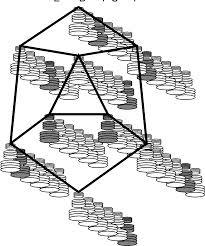
\includegraphics[scale=0.9]{BunchGraph}
\caption{Representación de Face Graph presentada en \cite{wiskott1997face} }
\label{im:FaceGraph}
\end{figure}

Al final solo se hace una comparación punto a punto entre dos Face Graph para el proceso de reconocimiento.

\subsection{Función de similitud}
El proceso de reconocimiento se lleva a cabo mediante una función de similitud que compara cuan iguales son dos Face Graph, dicha función se expresa de la siguiente forma:
\begin{equation}
\label{FaceGraphSimiFunc}
L_{jet}(G,G')=\frac{1}{N}\sum_{i=0}^{N}S(J_{i},J'_{i})
\end{equation}
Donde $N$ es el numero de puntos fiduciales y $J_i,J'_i$ son los i-ésimos Gabor Jet que pertenecen respectivamente a los Face Graph $G,G'$ que van a ser comparados.

La función de similitud entre dos Gabor Jet es la siguiente:
\begin{equation}
\label{GaborJetSimiFunc}
S(J,J')=\frac{\sum_{j=1}^{N}a_j a'_jcos(\phi_j-\phi'_j)}{\sqrt{\sum_{j=1}^{N}a_j^2 \sum_{j=1}^{N}{a'}_j^2}}
\end{equation}

%escribir un parrafo sobre la comparacion de givens
Después de explicar el funcionamiento de \ac{EBGM} es necesario mencionar las situaciones donde tiene problemas para funcionar, según \cite{givens2004features} en su estudio comparativo con \ac{PCA} donde explica varias pruebas. Cuando hay cambios bruscos de expresión, cambio de los ojos y boca, y ojos cerrados son las situaciones en las cuales \ac{EBGM} tiene problemas para realizar el reconocimiento, finalmente concluye que dichos problemas tienen en parte relación con el hecho que se necesita las coordenadas de los ojos para empezar el reconocimiento y las dificultades relacionadas para encontrar dichas posiciones afectan el desempeño del algoritmo.

%parrafo para terminar la seccion
En esta sección se explicó el funcionamiento de \ac{EBGM} que extrae característica de partes bien definidas del rostros, que también son conocidas como características biométricas.

%En un contexto de vídeo vigilancia no solo hace falta elegir un método de reconocimiento de rostros, también en necesario establecer que características van a ser medidas y como ellas van a ser identificadas por ello es necesario explicar el concepto de reconocimiento biométrico.

\section{Consideraciones finales}
En este capítulo se ha expuesto todos los métodos que interviene en alguna u otra forma en la propuesta, se ha presentado una introducción a cada una de ellos.

Es necesario resaltar que \ac{EBGM} es un método de reconocimiento biométrico, que se refiere a una forma de reconocimiento basado en un vector de características que derivan mayormente de características biológicas, se considera mucho mas confiable que otros métodos de reconocimiento que usan claves, contraseñas, tarjetas, etc \cite{alice2003biometric}. Esto se debe a cumple con los requerimientos necesarios para ser considerado como tal siendo estos los siguientes:

\begin{itemize}
\item Universalidad.- Toda persona debe tener dicha característica.
\item Distintividad.- Cualquier par de personas debe ser diferente en términos de dicha característica
\item Permanencia.-La característica debe ser lo suficientemente invariable a lo largo del tiempo para que pueda ser usada como criterio de comparación.
\item Medible.-La característica debe ser cuantitativamente mensurable.
\end{itemize}

Por ello es adecuado su uso para un escenario de vídeo vigilancia en el cual se aplica la propuesta presentada en el siguiente capítulo.


\chapter{Marco teórico de la propuesta}\label{chap:Conceptos}
En este capítulo se presenta todos los conceptos y técnicas usadas para el desarrollo de la propuesta desde las técnicas de detección usadas hasta el proceso de reconocimiento.

\section{Métodos de detección}

Es necesario resaltar la importancia de una detección adecuada para el reconocimiento ya que ambos son procesos muy relacionados entre sí. En esta sección se explican tres métodos de detección uno para encontrar rostros, otro para validar los rostros detectados y finalmente uno para encontrar puntos de dentro de los rostros.


\subsection{Detector de Viola-Jones}\label{scc:Viola}
El detector de Viola-Jones también conocido como \textit{Haar Detector} en implementaciones libres, se presenta en \cite{viola2001rapid} donde se hace uso de las características Haar (Figura \ref{im:Haar}) en una representación conocida como Imagen Integral, también se utiliza el Algoritmo Ada Boost y un clasificador en casada para completar el proceso de detección.

\begin{figure}[h]
\center
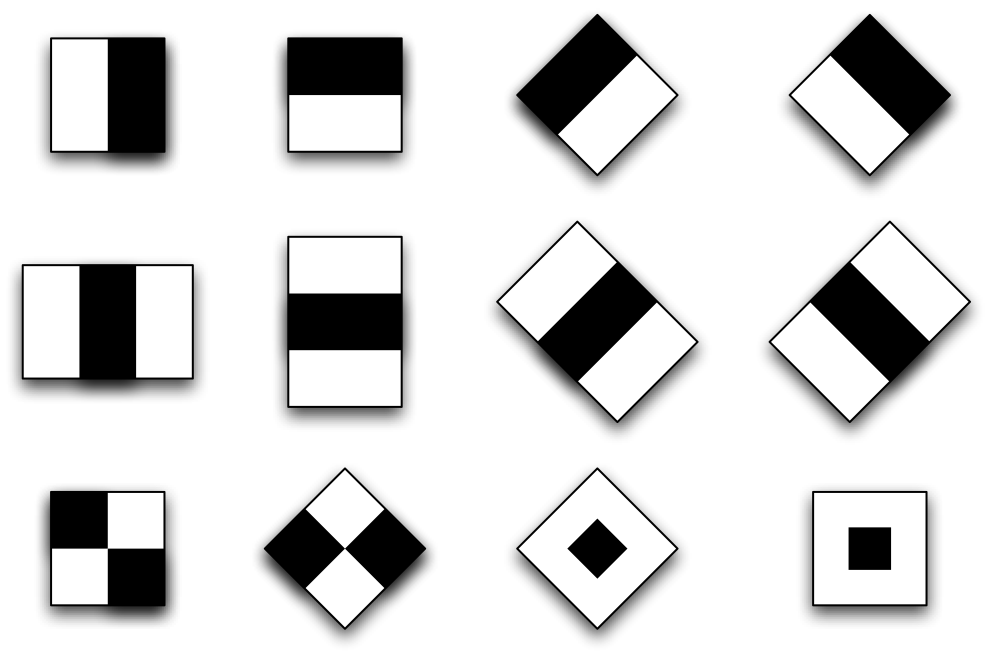
\includegraphics[scale=.5]{Haar}
\caption{Ejemplo de característica Haar, extraído de \cite{viola2001rapid}. Estos rectángulos pueden ser entendidos como rectángulos en los cuales son determinados como áreas de baja iluminación y otros como áreas de alta iluminación de esta manera podemos representar el contraste entre dos secciones de la imagen,}
\label{im:Haar}
\end{figure}

En \cite{viola2001rapid} se explica que el trabajo de detección se basa en tres conceptos:
\subsubsection{Imagen integral}
Usa un concepto parecido a una tabla de texturas donde tenemos en cada punto el valor de la suma de los pixeles de arriba y a la derecha de dicho punto. 

Esto permite el calculo rápido de valor de los pixeles para cualquier sección de la imagen, dicho valor nos ayuda a hacer un calculo rápido del contraste en cualquier sección, lo cual permite el calculo de cualquier característica Haar en tiempo constante.
\subsubsection{Algoritmo Ada Boost}
Debido a la existencia de un gran numero de características Haar, aproximadamente más de 45,000 no es posible usar todas en un proceso de clasificación, por lo que es necesario encontrar un conjunto pequeño de características que juntas formen un clasificador efectivo.

En \cite{viola2001rapid} se presenta una modificación al algoritmo Ada Boost para seleccionar las mejores características Haar y con ellas entrenar varios clasificadores débiles en términos de su tasa de aciertos, que en combinación permiten obtener un clasificador fuerte. De esta manera tener un clasificado robusto para el proceso de detección.
\subsubsection{Clasificador en casada}
La idea tras un clasificador en cascada es organizar todos los clasificadores débiles en un estilo en el cual estén uno detrás de otro como una cascada. Cuando se analiza una región esta pasa por el primer clasificador y sí el resultados es negativo se descarta, pero si resulta positivo pasa al siguiente clasificador hasta el final de la cascada y así sucesivamente de esta manera obtiene un solo clasificador, más robusto que los clasificadores que lo componen. Este proceso se puede apreciar en la Figura \ref{im:cascade}.

\begin{figure}[h]
\center
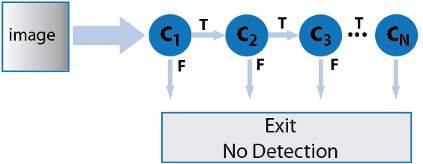
\includegraphics[scale=0.75]{cascadeClassifier}
\caption{Muestra del clasificador en cascada, donde una imagen es analizada por un clasificador tras otro desde el primero hasta el n-esimo si resulta la imagen positiva, extraído de \cite{viola2001rapid}.}
\label{im:cascade}
\end{figure}

El detector de Viola-Jones es ampliamente usado y reconocido como un detector que entrega una gran cantidad de verdaderos positivos (detecciones acertadas). Pero es necesario mencionar sus limitaciones y falencias, de la misma manera que entrega un gran porcentaje de verdaderos positivos también entrega falso  positivos (detecciones presentadas como verdaderas pero que no lo son) esto es debido a que el calculo de la imagen integral se hace en la escala de grises a veces alguna configuración de sombras producidas en la imagen genera la misma distribución de contrastes que un rostro humano.

Otro defecto es que solo detecta rostro de frente. No puede detectar otras posiciones del rostro humano simultáneamente. A pesar de estas deficiencia sigue siendo usado no solo para rostros sino para otro tipo de objetos ya que su mayor ventaja es que es entrenarle.

\subsection{Detector de \acf{HOG}}
Un detector de \acf{HOG} usa una combinación del descriptor de \ac{HOG} y un clasificador basado en \acf{SVM}, originalmente usado para detectar personas \cite{dalal2005histograms}, su uso se ha incrementado a varias situaciones, incluyendo la detección de rostros, a continuación exponemos las ideas detrás de este detector.
\subsubsection{Descriptor de \ac{HOG}}
Un descriptor de \ac{HOG} muestra el calculo de la gradiente de una imagen, la gradiente es cambio de la intensidad de la imagen en una cierta dirección, pudiendo ser representado como un vector que posee magnitud $g$ y dirección $\theta$, el calculo del gradiente en una imagen se hace por pixel y retorna la dirección del cambio y su magnitud, este proceso se observa en las siguientes ecuaciones:
\begin{equation}
dx=I(x+1,y)-I(x-1,y)
\end{equation}
\begin{equation}
dy=I(x,y+1)-I(x,y-1)
\end{equation}
\begin{equation}
\theta(x,y)=arctan\left(\frac{dy}{dx}\right)
\end{equation}
\begin{equation}
g(x,y)=\sqrt[2]{dx^2+dy^2}
\end{equation}

Donde $x$ y $y$ son las coordenadas de la imagen y la función $I(x,y)$ es el valor del pixel o intensidad en dichas coordenadas. Luego se divide la imagen en secciones iguales y en cada una de estas secciones se calcula un histograma de las orientaciones para conocer la orientación dominante de cada sección, de esta manera creamos un vector de características.

Con esta información se puede describir el contorno y forma de una figura, lo que es útil para realizar una clasificación.

\subsection{\acf{SVM}}
Un \ac{SVM} \cite{cortes1995support} es un clasificador lineal en el cual se intenta crear una linea divisoria entre las representación (vectores de características) de ejemplos positivos y negativos de un objeto determinado.

Esta basado en el aprendizaje estadístico para resolver problemas de clasificación de patrones. Los clasificadores lineales se caracterizan porque aprenden una función lineal para separar las clases. No se trata de una agrupación por similitudes, sin que existe una separación definida entre clases.

Dado un conjunto de ejemplos de entrenamiento (muestras) podemos etiquetar las clases y entrenar una SVM para construir un modelo que prediga la clase de una nueva muestra. Intuitivamente, una SVM es un modelo que representa a los puntos de muestra en el espacio, separando las clases por una linea representada por la función del clasificador. Cuando las nuevas muestras se ponen en correspondencia en función de su proximidad, pueden ser clasificadas a una u otra clase, dependiendo de la proximidad a cada una. Mas formalmente, la idea principal de SVM es construir un hiperplano o conjuntos de hiperplanos en un espacio de dimensionalidad muy alta como superficie de decisión, de tal forma que, el margen de separación entre ejemplos positivos y negativos sea el máximo. Una buena separación entre las clases permitirá una clasificación correcta. 

\ac{SVM} resulta ser un clasificador muy robusto y usado, el cual presenta varias modificaciones alrededor del estado del arte.


\subsection{\acf{CLNF}}
\ac{CLNF} es un método para encontrar puntos de interés en imágenes de rostros presentado en \cite{baltrusaitis2013constrained} e implementado para aplicaciones de video en \cite{Baltrusaitis2016} en la presentación de su framework ``Open Face'' para el tracking y detección de rostros, donde publica el código de su propuesta, \ac{CLNF} se basa en \ac{CLM}, por lo tanto empezamos con una explicación de \ac{CLM}.

\ac{CLM} es una forma para localizar un conjunto de puntos restringido por un modelo en una imagen, el proceso consiste en tomar una muestra de una área de la imagen donde se realizó una estimación inicial proyectarla a un marco de referencia. Por cada punto se genera una imagen de respuesta donde se le da una puntuación por tener el punto a localizar en cada pixel. Este puntaje es determinado a través de un detector local que evalúa el punto según un modelo de distribución de puntos en donde penaliza distribuciones complicadas y premia distribuciones simples y mas probables, de esta manera se evalúan todos los puntos en conjunto.

En \cite{baltrusaitis2013constrained} se propone el uso de redes neuronales para los detectores locales de los puntos, con lo cual logra una mejor determinación de puntos en relación con el resto de puntos detectados. Compara sus resultados con otras técnicas del estado del arte así mismo realiza pruebas con imágenes obtenidas de Internet que presentan condiciones no controladas.

\section{Técnicas de pre-procesamiento}
Como se puede observar en las secciones anteriores un problema en especial difícil es la iluminación, por lo que es necesario hablar sobre las técnicas de pre-procesamiento, se entiende como pre-procesamiento a las técnicas que modifican una imagen para acentuar alguna característica, estas serán usadas para afrontar dicho problema.

\subsection{Ecualización de histograma}
Las ecualización del histograma de una imagen es una transformación que pretende obtener para una imagen un histograma con una distribución uniforme. Es decir, que exista el mismo número de pixeles para cada nivel de gris del histograma de una imagen monocroma \cite{orlova2002image}.
La función de la ecualización es:
\begin{equation}
h(v)=Redondeo\Bigg(\frac{cdf(v)-cdf_{min}}{(M\times N)-cdf_{min}} \times (L-1)\Bigg)
\end{equation}
Donde $cdf_{min}$ es el mínimo valor no nulo de la función de distribución de acumulación. $M\times N$ es el numero de pixeles en la imagen y $L$ es el numero de niveles de la escala de gris.

\begin{figure}[h]
\center
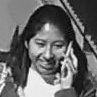
\includegraphics[scale=1]{face_original}
\hspace{1cm}
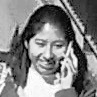
\includegraphics[scale=1]{face_he}
\caption{Ecualización de histograma - Izquierda: imagen en escala de Grises. Derecha: imagen ecualizada.}
\label{im:he}
\end{figure}


\subsection{Transformada de logaritmo}
La Transformada de logaritmo asigna un rango estrecho de valores (píxeles en escala de grises o un canal de un espacio de color) de un rango amplio de valores de entrada. La transformada de logaritmos es útil si se necesita expandir los valores de píxeles oscuros de una imagen mientras se comprime los valores altos \cite{thamiz2015liter}

\begin{equation}
\label{f_log}
s = c*log(1+ 256*r)
\end{equation}

Donde $r$ es la imagen de entrada, $c$ es una constante, $s$ es la imagen mejorada. Para la transformada de logaritmo se utilizo el valor de 20 para la constante $ c $. 

\begin{figure}[h]
\center
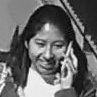
\includegraphics[scale=1]{face_original}
\hspace{1cm}
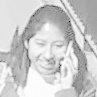
\includegraphics[scale=1]{face_log}
\caption{Transformada de logaritmo - Izquierda: imagen en escala de Grises. Derecha: imagen con Transformada de logaritmo.}
\label{im:log}
\end{figure}

\subsection{Transformada discreta de coseno}
La transformada Discreta de coseno (DCT por sus siglas en ingles) es utilizada especialmente en el procesamiento de señales e imágenes. DCT expresa en una secuencia finita de puntos, datos en términos de sumas de funciones de coseno en diferentes frecuencias. En el procesamiento de imágenes, la utilización de DCT ayuda a descomponer una imagen en frecuencias, donde usualmente los pequeños componentes de frecuencia altas pueden ser descartados. La ecuación en 2D está dada por la Ecuación. \ref{f_dct}
\cite{thamiz2015liter}\cite{vish2015ill}

\begin{equation}
	\label{f_dct}
	\resizebox{0.91\hsize}{!}{
		$ C(u,v) = \alpha(u)\alpha(v)\sum\limits_{x=0}^{N-1} \sum\limits_{y=0}^{N-1}f(x,y)cos\left[\frac{\pi(2x + 1)u}{2N}\right]cos\left[\frac{\pi(2y + 1)v}{2N}\right] $
	}
\end{equation}

Donde: $u$, $v$, $N$, $\alpha(u)$ y $\alpha(v)$ se definen de igual forma que la ecuación 1D. La ecuación inversa está definida por la Ecuación. \ref{f_idct}.

\begin{equation}
	\label{f_idct}
	\resizebox{0.91\hsize}{!}{
		$ f(x,y) = \sum\limits_{x=0}^{N-1}\sum\limits_{y=0}^{N-1} \alpha(u)\alpha(v)C(u,v)cos\left[\frac{\pi(2x + 1)u}{2N}\right]cos\left[\frac{\pi(2y + 1)v}{2N}\right]$
	}
\end{equation}

El resultado de la transformada de coseno, es una matriz de coeficientes positivos y negativos, los cuales representan la adición o resta de una determinada frecuencia para generar la imagen procesada por la transformada discreta de Coseno.

%parrafo para dar conclusion a la seccion
Se ha expuesto tres técnicas de pre-procesamiento que serán usadas en usadas en la propuesta del Capítulo \ref{chap:Propuesta}, todas abordan el problema de la iluminación de manera diferente, es necesario tener en cuenta que este problema ha sido tratado mucho en el estado del arte pero aun no se encuentra una técnica de mejora de iluminación sea robusta en cualquier escenario.

%En la siguiente sección se expone los métodos de detección usados como parte de nuestra propuesta. Se explica su funcionamiento y su posición en el estado del arte.


\section{\acf{EBGM}}\label{scc::EBGM}
%Después de haber tratado los métodos de pre-procesamiento, finalmente se expone las técnica de reconocimiento de rostro que en el Capítulo \ref{chap:Propuesta} se presenta una modificación.

\ac{EBGM} presentado en \cite{wiskott1997face} se basa en el concepto que las imágenes de los rostros reales tienen muchas características no lineales que no son abordadas por los métodos de reconocimiento holísticos, tales como variaciones en la iluminación, pose y expresión.
También se apoya en el argumento que las características visuales que se basan en Gabor Wavelet, han probado ser un buen modelo del procesamiento visual temprano en el cerebro, más precisamente células simples en la corteza visual primaria, por ello también se considera un algoritmo inspiración biológica.

Para ello, una transformación de Gabor wavelet crea una arquitectura de enlaces dinámicos que proyecta el rostro en una malla elástica que es conocida como Face Graph.
El Gabor Jet es un nodo en la malla elástica, el cual describe el comportamiento alrededor de un pixel. Esto es el resultado de la convolución de una imagen con varias máscaras de Gabor, el cual es usado para detectar formas y extraer características.

El reconocimiento esta basado en la similaridad de la respuesta mascara de Gabor a cada nodo. La dificultad con este método es el requerimiento de marcar puntos precisos en los rostros.

A continuación se explica en detalle su funcionamiento

\subsection{Gabor Wavelet}\label{sscc:GaborWavelet}
Las Gabor Wavelet son funciones que modifican las imágenes en el espacio de las frecuencias. El espacio de las frecuencia esta estrechamente relacionado al análisis de Fourier, por lo que es necesario hacer una breve descripción.

Una transformada de Fourier descompone una señal de tal manera que pueda ser representada como una combinación de sinusoidales. Cuando se procesa señales como lo pueden ser las imágenes, son representadas como una longitud de onda, ello es muy útil ya que revela información que no puede ser vista cuando observamos la imagen original.

Mientras una señal es un función en base al tiempo, la transformada de Fourier es una función en base a la frecuencia, se puede observar la transformada de Fourier en una dimensión en la siguiente ecuación:

\begin{equation}
F(x(t))(\omega)=\int_{-\infty }^{\infty } x(t)e^{-i\omega t}dt
\end{equation}

En la transformada de Fourier y en los Gabor Wavelet la función comprende una parte imaginaria y una real:

\begin{equation}
F(x(t))(\omega)=\int_{-\infty }^{\infty } x(t)cos(\omega t)dt - i\int_{-\infty }^{\infty } x(t)sen(\omega t)dt
\end{equation}

Cuando una transformada de Fourier se aplica una frecuencia en particular el resultado es un numero complejo que corresponde a la amplitud del coseno y del seno de la función original, en cada frecuencia hay un componte real y otro imaginario.

Las Gabor Wavelet son como la transformada de Fourier solo que tiene un alcance limitado, básicamente son una sinusoidal multiplicada por una Gaussiana.

Cuando una función es convolucionada con un Gabor Wavelet la información más cerca al centro de la campana de la Gaussiana es la que es tomada en cuenta mientras la más lejana es ignorada.

La ecuación de una de una Gabor Wavelet es la siguiente:
\begin{equation}
W(t,t_0,\omega)=e^{-\sigma(t-t_0)^2} e^{--i\omega(t-t_0)}
\end{equation}
y su convolucion es:
\begin{equation}
C(x(t))(t_0,\omega)=\int_{-\infty}^{\infty}x(t)W(t,t_0,\omega)dt
\end{equation}

De la misma manera que Fourier produce una resultado complejo un Gabor Wavelet produce:
\begin{equation}
C(x(t))(t_0,\omega)=a_{real}+ia_{imag}
\label{ec:ConvolucionWavelet}
\end{equation}

Mientras las ecuaciones presentadas hasta ahora trabajan en una dimensión es necesario presentar una forma en la que se pueda trabajar en dos dimensiones, esta es la representación del Gabor Wavelet como mascara para una convoluciónn en imágenes.

La Ecuación \ref{GaborWavelet} define como crear una máscara de Gabor donde $x, y$ son las posiciones en la mascara, para cualquier tamaño de mascara.
%El Gabor Jet es un nodo en la malla elástica, el cual describe el comportamiento alrededor de un pixel. Esto es el resultado de la convolución de un pixel de la imagen con varios Gabor wavelet o máscaras de Gabor, los cuales son usados para detectar formas y extraer características.

\begin{equation}
W(x,y,\theta,\lambda, \phi, \sigma, \gamma )=e^{-\frac{x'^2+\gamma y'^2}{2 \sigma^2}}cos(2\pi \frac{x'}{\lambda}+\phi) 
\label{GaborWavelet}
\end{equation}
\begin{equation*}
x'=cos\theta+ysin\theta   
\label{GaborWaveletx}
\end{equation*}
\begin{equation*}
y'=-x sin\theta+ycos\theta
\label{GaborWavelety}
\end{equation*}
Los parámetros usados para la construcción de los Gabor wavelet son los mismo que se utilizan en la implementación de \cite{bolme2003elastic}, a continuación los explicamos brevemente:
\begin{itemize}
\item $\theta$ especifica la orientación del Gabor Wavelet.\\
Siendo $\theta \in \left\{0,\pi/8,2\pi/8,3\pi/8,4\pi/8,5\pi/8,6\pi/8,7\pi/8 \right\}$
\item $\lambda$ especifica el ancho de onda de la función seno, empieza con 4 pixeles y aumenta en medias octavas siendo $\lambda \in \left\{4,4\sqrt{2},8,8\sqrt{2},16\right\} $
\item $\phi$ especifica la fase de la función seno, pudiendo ser par e impar que representa la parte imaginaria y la parte real del wavelet respectivamente.
Siendo $\left\{0,\pi/2\right\}$
\item $\delta$ especifica el radio de la Gaussiana. En este caso $\delta=\lambda$.
\item $\gamma$ especifica el ratio de aspecto de la Gaussiana. Este parámetro es incluido para que el Wavelet se aproxime a ciertos modelos biológicos. Siendo $\gamma=1$.
\end{itemize}


De esta manera podemos crear varios tamaños de máscaras que en la configuración original son $N \in \left\{25, 37, 51, 71, 101 \right\}$. Dando 80 configuraciones de Gabor wavelet y siendo efectivas 40 máscaras por punto, debido a que existe una mascara que extraer la parte imaginara y otra la parte real del Wavelet.
%buscar imagen de las mascaras

Al conjunto coeficientes (reales e imaginarios) producidos por estas mascaras de Gabor son llamados Gabor Jet que son el corazón de todo el proceso de reconocimiento de \ac{EBGM}.

A continuación se explica como es el proceso por el cual \ac{EBGM} determina en que puntos de una imagen va extraer características. A estos punto se les conocen como puntos fiduciales.

\subsection{Localización de puntos fiduciales}
Como se menciona en la sección anterior la convolución del conjunto de mascaras de Gabor sobre un punto produce un Gabor Jet que es un conjunto de coeficientes.

\begin{figure}[h]
\center
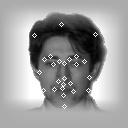
\includegraphics[scale=1.5]{Points}
\caption{Muestra de los puntos fiduciales elegidos en \ac{EBGM}\cite{bolme2003elastic}, en cada punto se realiza 40 convoluciones con máscaras de Gabor para crear un Gabor Jet por punto}
\label{im:puntos}
\end{figure}

Siguiendo el trabajo de \cite{wiskott1997face}, Bolme realiza una implementación de código libre de todo el algoritmo y da un mayor detalle de su funcionamiento, listando que puntos de interés debemos encontrar en una imagen. Estos puntos son conocidos como puntos fiduciales, en el Cuadro \ref{ta:PuntosFiduciales} se puede observar una lista de ellos, y en la Figura \ref{im:puntos} se puede ver su localización.

\begin{table}[h]
\centering
\caption{Lista de puntos fiduciales presentada en \cite{bolme2003elastic}}
\label{ta:PuntosFiduciales}
\begin{tabular}{|l|l|}
\hline
1. Ojo izquierdo                          & 2. Ojo derecho                          \\ \hline
3. Centro del puente de la nariz          & 4. Pico de la ceja izquierda            \\ \hline
5. Pico de la ceja derecha                & 6. Interior de la ceja izquierda        \\ \hline
7. Interior de la ceja derecha            & 8. Exterior de la ceja izquierda        \\ \hline
9. Exterior de la ceja derecha            & 10. Centro de la punta de la nariz      \\ \hline
11. Centro de la base de la nariz         & 12. Izquierda de la base de la nariz    \\ \hline
13. Derecha de la base de la nariz        & 14. Centro parte superior boca          \\ \hline
15. Centro parte inferior boca            & 16. Esquina izquierda de la boca        \\ \hline
17. Esquina derecha de la boca            & 18. Parte central del tope de la cabeza \\ \hline
19. Parte izquierda del tope de la cabeza & 20. Parte derecha del tope de la cabeza \\ \hline
21. Costado izquierdo del rostro          & 22. Costado derecho del rostro          \\ \hline
23. Centro de la barbilla                 & 24. Quijada izquierda                   \\ \hline
25. Quijada derecha                       &                                         \\ \hline
\end{tabular}
\end{table}

El método por el cual \ac{EBGM} encuentra los puntos fiduciales es a través del uso de moldes, imágenes en  las cuales los puntos han sido encontrados manualmente. En los trabajos de \cite{wiskott1997face} y \cite{bolme2003elastic} utilizan 70 imágenes normalizada a un mismo tamaño y donde las coordenadas de los ojos son las mismas.

Sobre cada imagen de molde y en cada punto marcado se realiza las convoluciones de las mascaras de Gabor para producir un Gabor Jet, de esta manera todos los puntos en todas las imágenes tienen un Gabor Jet. Finalmente todos los Gabor de un punto, por ejemplo el ojo izquierdo, son reunidos en un solo grafo conocido como Bucnh Graph que contiene todos los Gabor Jet de los modelos.

De esta manera se obtiene un modelo general con información de todos los modelos, también contiene la información de coordenada de cada punto en cada modelo y un punto de coordenada promedio.

Para reconocer una nueva imagen se realiza una normalización de tamaño y una traslación coordenadas de los ojos a coordenadas preestablecidas a través de una transformación matricial. Mediante un alineamiento entre las coordenadas normalizadas de los ojos y las coordenadas de los ojos del Bunch Graph se encuentran el resto de los puntos fiduciales en la imagen usando la información de coordenada promedio almacenada en el Bunch Graph. Finalmente se encuentra la posición final del punto usando como referencia el Gabor Jet con mayor similaridad en el Bunch Graph

Según \cite{bolme2003elastic} y \cite{wiskott1997face}, y como se menciona en la sección anterior el resultado de una transformada de Fourier en una función y en una frecuencia determinada es un numero complejo, que tiene una correspondencia en amplitud en términos de senos y cosenos que pueden ser representada como una coordenada polar.
\begin{equation}
x_{\omega}(t)=a_{\omega,r}cos(t)+a_{\omega,i}sin(t)= a cos(t+\phi).
\label{ec:CorrepondeciaAPolar}
\end{equation}
Es posible representar las suma de las sinusoidales como una función coseno dándole una amplitud y fase especifica.
Esto sucede cuando las sinusoidales son multiplicadas por una Gaussiana como se observa en la Ecuación \ref{ec:ConvolucionWavelet} y según lo visto en la Ecuación \ref{ec:CorrepondeciaAPolar} se puede representar los coeficientes complejos del resultado de las convoluciones como coordenadas polares de magnitud $a$ y un angulo $\phi$
\begin{equation}
a_{real} = a cos\phi 
\end{equation}
\begin{equation}
 a_{imag} = a sen\phi 
\end{equation}
y podemos halla $a$ y $\phi$ mediante:
\begin{equation}
a = \sqrt{a^2_{real}+a^2_{imag}}
\end{equation}
\begin{equation}
\phi=\left\{\begin{matrix}
arctan(a_{imag}/a_{real}) & \textrm{si } a_{real}>0 \\ 
\pi+arctan(a_{imag}/a_{real}) & \textrm{si } a_{real}<0 \\ 
\pi/2 & \textrm{si } a_{real}=0 \textrm{ y } a_{imag}>= 0 \\ 
-\pi/2 & \textrm{si } a_{real}=0 \textrm{ y } a_{imag}<0
\end{matrix}\right.
\end{equation}
Gracias a esta transformación a coordenadas polares podemos representar la información compleja del resultado de la convolucion de una mascar de Gabor. 
%Existe una relación entre el desplazamiento de tiempo en frecuencia y el angulo de la fase del coeficiente. Sí los coeficientes de dos puntos separados por un pequeño desplazamiento son calculados, la diferencia entre el angulo de la fase de dichos puntos debe ser proporcional al desplazamiento entre dichos puntos.

%De esta manera solo se convolusiona el punto una vez, cuando se hace la estimacion inicial y se elige el Gabor Jet mas parecido del Bunch Graph y sobre el se calcula el desplazamiento así para calcular la posición final del punto fiducial, este proceso es el que le da el nombre de \textit{elastic} a \ac{EBGM}.

Cabe mencionar que la mayor debilidad del algoritmo yace en este proceso ya que si el alineamiento del grafo falla por culpa de un error en las coordenadas de los ojos el resto de las estimaciones iniciales falla. % y a pesar de tener una función para el calculo de desplazamiento está limitada a pequeños desplazamientos y búsquedas locales ya que no es practico que haga las estimación a lo largo de grande porciones de la imagen.
Otra dificultad que presenta es la dependencia a sus modelos, esto quiere decir que por ejemplo si entre sus modelos no se encuentra alguien con barba cuando se intente encontrar puntos en nueva imagen de una persona con barba no va existir ningún Gabor Jet en el Bunch Graph que sea una buena referencia para el ajuste de la posición final del punto.

Finalmente es necesario contar con las coordenadas de ojos de antemano, este hecho por simple que parezca es una de las limitaciones para que \ac{EBGM} se pueda usar en un sistema de reconocimiento de rostro automatizado sobre todo en vídeo vigilancia donde encontrar ojos es difícil.

\subsection{Face Graph}
Una vez hallada la posición final de los puntos se extrae los coeficientes finales (la representación en coordenadas polares de la convolucion) para los Gabor Jet donde se almacenan una estructura que se conoce como Face Graph. A pesar que en la literatura se representa como un grafo , Figura \ref{im:FaceGraph} , Un Face Graph en realidad es un vector de características.
\begin{figure}[h]
\center
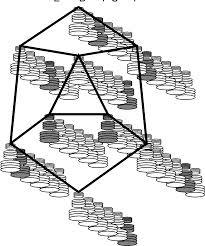
\includegraphics[scale=0.9]{BunchGraph}
\caption{Representación de Face Graph presentada en \cite{wiskott1997face} }
\label{im:FaceGraph}
\end{figure}

Al final solo se hace una comparación punto a punto entre dos Face Graph para el proceso de reconocimiento.

\subsection{Función de similitud}
El proceso de reconocimiento se lleva a cabo mediante una función de similitud que compara cuan iguales son dos Face Graph, dicha función se expresa de la siguiente forma:
\begin{equation}
\label{FaceGraphSimiFunc}
L_{jet}(G,G')=\frac{1}{N}\sum_{i=0}^{N}S(J_{i},J'_{i})
\end{equation}
Donde $N$ es el numero de puntos fiduciales y $J_i,J'_i$ son los i-ésimos Gabor Jet que pertenecen respectivamente a los Face Graph $G,G'$ que van a ser comparados.

La función de similitud entre dos Gabor Jet es la siguiente:
\begin{equation}
\label{GaborJetSimiFunc}
S(J,J')=\frac{\sum_{j=1}^{N}a_j a'_jcos(\phi_j-\phi'_j)}{\sqrt{\sum_{j=1}^{N}a_j^2 \sum_{j=1}^{N}{a'}_j^2}}
\end{equation}

%escribir un parrafo sobre la comparacion de givens
Después de explicar el funcionamiento de \ac{EBGM} es necesario mencionar las situaciones donde tiene problemas para funcionar, según \cite{givens2004features} en su estudio comparativo con \ac{PCA} donde explica varias pruebas. Cuando hay cambios bruscos de expresión, cambio de los ojos y boca, y ojos cerrados son las situaciones en las cuales \ac{EBGM} tiene problemas para realizar el reconocimiento, finalmente concluye que dichos problemas tienen en parte relación con el hecho que se necesita las coordenadas de los ojos para empezar el reconocimiento y las dificultades relacionadas para encontrar dichas posiciones afectan el desempeño del algoritmo.

%parrafo para terminar la seccion
En esta sección se explicó el funcionamiento de \ac{EBGM} que extrae característica de partes bien definidas del rostros, que también son conocidas como características biométricas.

%En un contexto de vídeo vigilancia no solo hace falta elegir un método de reconocimiento de rostros, también en necesario establecer que características van a ser medidas y como ellas van a ser identificadas por ello es necesario explicar el concepto de reconocimiento biométrico.

\section{Consideraciones finales}
En este capítulo se ha expuesto todos los métodos que interviene en alguna u otra forma en la propuesta, se ha presentado una introducción a cada una de ellos.

Es necesario resaltar que \ac{EBGM} es un método de reconocimiento biométrico, que se refiere a una forma de reconocimiento basado en un vector de características que derivan mayormente de características biológicas, se considera mucho mas confiable que otros métodos de reconocimiento que usan claves, contraseñas, tarjetas, etc \cite{alice2003biometric}. Esto se debe a cumple con los requerimientos necesarios para ser considerado como tal siendo estos los siguientes:

\begin{itemize}
\item Universalidad.- Toda persona debe tener dicha característica.
\item Distintividad.- Cualquier par de personas debe ser diferente en términos de dicha característica
\item Permanencia.-La característica debe ser lo suficientemente invariable a lo largo del tiempo para que pueda ser usada como criterio de comparación.
\item Medible.-La característica debe ser cuantitativamente mensurable.
\end{itemize}

Por ello es adecuado su uso para un escenario de vídeo vigilancia en el cual se aplica la propuesta presentada en el siguiente capítulo.


\chapter{Propuesta} \label{chap:Propuesta}
%parrafo de introduccion recordando objetivo
%La propuesta de este trabajo de tesis consiste en la adopción y adaptación de técnicas y trabajos ya existentes sobre los cuales, realizar las modificaciones que nos permita reconocer rostros en un contexto de vídeo vigilancia.

La propuesta de este trabajo presenta un \textit{pipeline} de reconocimiento de rostros en vídeo donde se usa \ac{EBGM} que ha sido elegido por sus resultado en comparativas realizadas con otros métodos holísticos, y por ser un método que es considerado biométrico por lo expuesto en los capítulos anteriores.

Cabe resaltar que la principal dificultad para su uso en vídeo vigilancia es su necesidad de tener las coordenadas de los ojos ya encontradas para poder determinar el resto de puntos fiduciales. Este hecho es especialmente importante ya que el proceso de estimación de puntos esta ligado a que tipos de modelos se usa y puede ser influenciado por algún patrón dentro de los modelos.

A pesar de la dificultad mencionada, \ac{EBGM} sigue siendo un algoritmo adecuado para el reconocimiento de rostros en vídeo vigilancia. Por ello se propone adoptar el uso de \ac{CLNF} para reemplazar el proceso de estimación de puntos fiduciales que \ac{EBGM} usa.

A continuación se presenta el esquema general de la propuesta de este trabajo de tesis.

\section{Esquema general de la propuesta}
%mostrar y describir las partes del pipe lines de vídeo
Para poder realizar el reconocimiento de rostros en vídeo vigilancia se debe establecer un \textit{pipeline} de procesos para alcanzar dicha meta, a continuación se describe los pasos necesarios para el reconocimiento de rostros:
\begin{enumerate}[label={[\arabic*]}]
\item Realizar la detección de rostros en la escena de vídeo vigilancia.
\item Validar dichas detecciones para descarta falsos positivos.
\item Encontrar puntos fiduciales en el rostro detectado.
\item Aplicar pre-procesamiento a la imagen de rostros detectada.
\item Normalizar imágenes de rostros a un tamaño y posición predefinida.
\item Realizar el proceso de reconocimiento usando \ac{EBGM}.
\item Mostrar el resultado del reconocimiento
\end{enumerate}
En la Figura \ref{im:PropPipeline} se puede observar la lista de procesos o \textit{pipeline} del procedimiento general de la propuesta desde adquisición de la imagen hasta el resultado del reconocimiento.
\begin{figure}[h]
\center
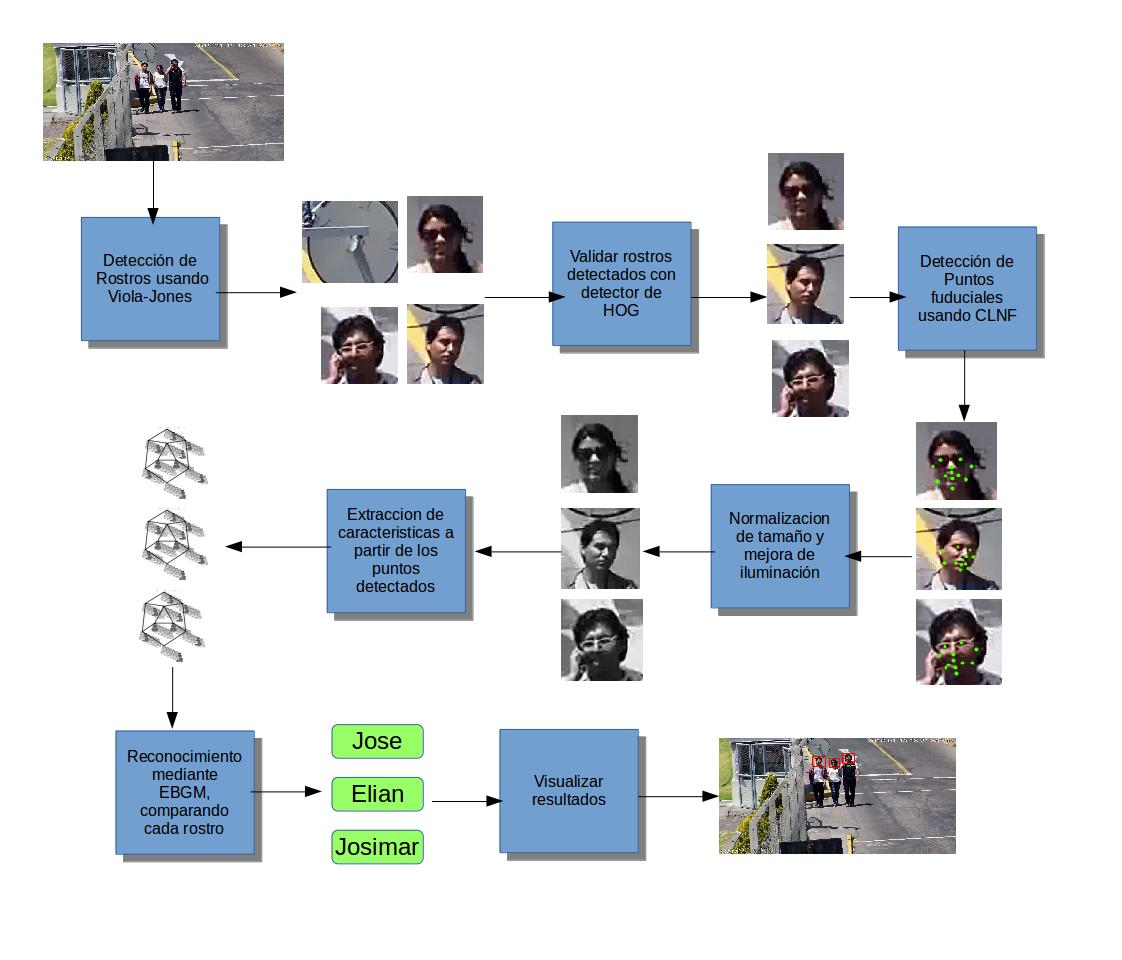
\includegraphics[scale=0.45]{Pipeline}
\caption{\textit{Pipeline} de propuesta, muestra el proceso de reconocimiento de rostros desde la detección en una escena hasta la muestra del resultado.}
\label{im:PropPipeline}
\end{figure}

En el Algoritmo \ref{alg:Propuesta} se describe el funcionamiento de nuestra propuesta donde se trata cada punto relevante:
\begin{algorithm}
\var{names} $\gets$ crear lista para almacenar nombres de imágenes de entrenamiento\;
\var{graphs} $\gets$ crear una lista de \var{FaceGraph}\;
\var{filter} $\gets$ crear un filtro de puntos fiduciales\;
\var{clnf\_model} $\gets$ leer y cargar modelo de entrenamiento para \ac{CLNF}\;
\var{mask} $\gets$ mascaras de Gabor a partir de un conjunto con parámetros\;
\var{trainSet} $\gets$ leer lista de direcciones y nombres de imágenes de entrenamiento\;
\ForEach{\var{element} en \var{trainSet}}
{
	\var{trainIm} $\gets$ leer imagen a partir de \var{element}\;
    \var{success} $\gets$ buscar puntos fiduciales en \var{trainIm} con \var{clnf\_model}\;
    \eIf{\var{success} es cierto}
    {
    	\var{faceLandmarkTrain} $\gets$ asignar lista de puntos fiduciales encontrados con \var{clnf\_model}\;
        añadir nombre de la imagen a la lista \var{names}\;
        \var{graph}$\gets$\textit{ConvertirImagenGrafo}(\var{trainIm},\var{faceLandmarkTrain},\var{mask},\var{filter})\;
    }
    {
    	escribir mensaje de error en entrenamiento\;
    }
}
\var{cascade} $\gets$ entrenar un clasificador basado en el algoritmo de Viola-Jones\;
\var{frame} $\gets$ leer \textit{frame} de vídeo de fuente\;
\If{fuente de vídeo no existe}
{
	escribir mensaje de error en fuente de vídeo y salir de la aplicación\;
}
\While{siempre cierto}
{
	\var{frame} $\gets$ leer desde fuente de vídeo\;
    \If{\var{frame} esta vacío}
    {
    	escribir mensaje de error\;
        salir de la aplicación\;
    }
    \var{frameGray} $\gets$ convertir \var{frame} a escala de grises\;
    detectar rostros en \var{frameGray} usando \var{cascade}\;
    \var{faces} $\gets$ guardar coordenadas de rostros detectados por \var{cascade}\;
    \ForEach{\var{element} en \var{faces}}
    {
    	\var{roi} $\gets$ recortar región de rostro en detectada en \var{frameGray} y validar detección con un detector de \ac{HOG}\;
        \var{success} $\gets$ buscar puntos fiduciales en \var{roi} con \var{clnf\_model}\;
    }
    \If{\var{var} es cierto}
    {
    	\var{var} $\gets$ asignar lista de puntos fiduciales encontrados con \var{clnf\_model}\;
        \var{detectedFace} $\gets$ ConvertirImagenGrafo(\var{roi},\var{faceLandmark},\var{mask},\var{filter})\;
    }
    ajustar \var{faceLandmark} a posición real en \var{frame}\;
    dibujar \var{faceLandmark} en \var{frame}\;
    dibujar recuadro de \var{roi} en \var{frame}\;
    \var{name} $\gets$ ReconocerFaceGraph(detectedFace,graphs,names)\;
    dibujar \var{name} sobre recuadro de \var{roi}\;
    visualizar \var{frame}\;
}
\caption{Pipeline de propuesta de reconocimiento de rostros}
\label{alg:Propuesta}
\end{algorithm}


\section{Detección y validación de rostros} 
Para el proceso de detección de rostros se utilizó el algoritmo de Viola-Jones, el cual devuelve regiones donde se detectaron rostros, es conocido que dicho algoritmo funciona bien en imágenes de alta resolución y condiciones de iluminación controladas. Como se observa en la Figura \ref{im:ViolaPerfect}, pero en el contexto de imágenes de vídeo vigilancia las cámara tiene menor resolución y no controlan la condiciones de iluminación, motivo por el cual nos da como resultados regiones que no necesariamente corresponden a un rostro (falsos positivos).

\begin{figure}[h]
\center
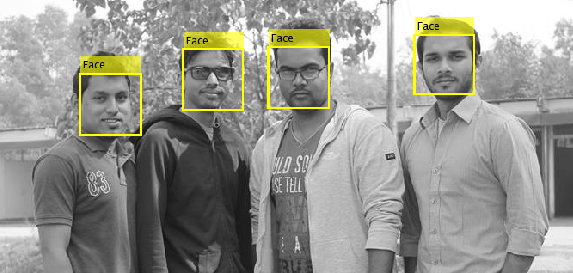
\includegraphics[scale=1]{ViolaPerfect}
\caption{Muestra de una imagen optima detector de Viola-Jones, todos los sujetos observan a la cámara y es una imagen en buena calidad, extraída de Internet}
\label{im:ViolaPerfect}
\end{figure}

Para que la propuesta sea robusta este trabajo presenta un validación mediante el descriptor de \ac{HOG}, de esta manera se mejora el proceso de detección a la vez de validar los resultados del detector de Viola-Jones. En general mejora la detección de rostros en sistemas de vídeo vigilancia.

\subsection{Detector de Viola-Jones}

El proceso de detección comienza con la transformación de la escena al espacio de imagen integral, como es explicado en la Sección \ref{scc:Viola}. Luego se analiza todas las regiones de la escena a través de una ventana para encontrar patrones de características Haar que cumplan con el entrenamiento del clasificador en cascada, dando como resultado las coordenadas de las regiones con rostros detectados. Este proceso se repite por varios tamaños de ventana diferente para detectar rostros en varios tamaños.

Como se observa en la Figura \ref{im:EscenaViola} y \ref{im:EscenaViolaResultados}, Viola-Jones tiene problemas en condiciones de iluminación no controladas, y se puede apreciar claramente que hay varios rostros detectados y un falso positivo. Motivo por el cual es necesario validar con el proceso siguiente.

\begin{figure}[h]
\center
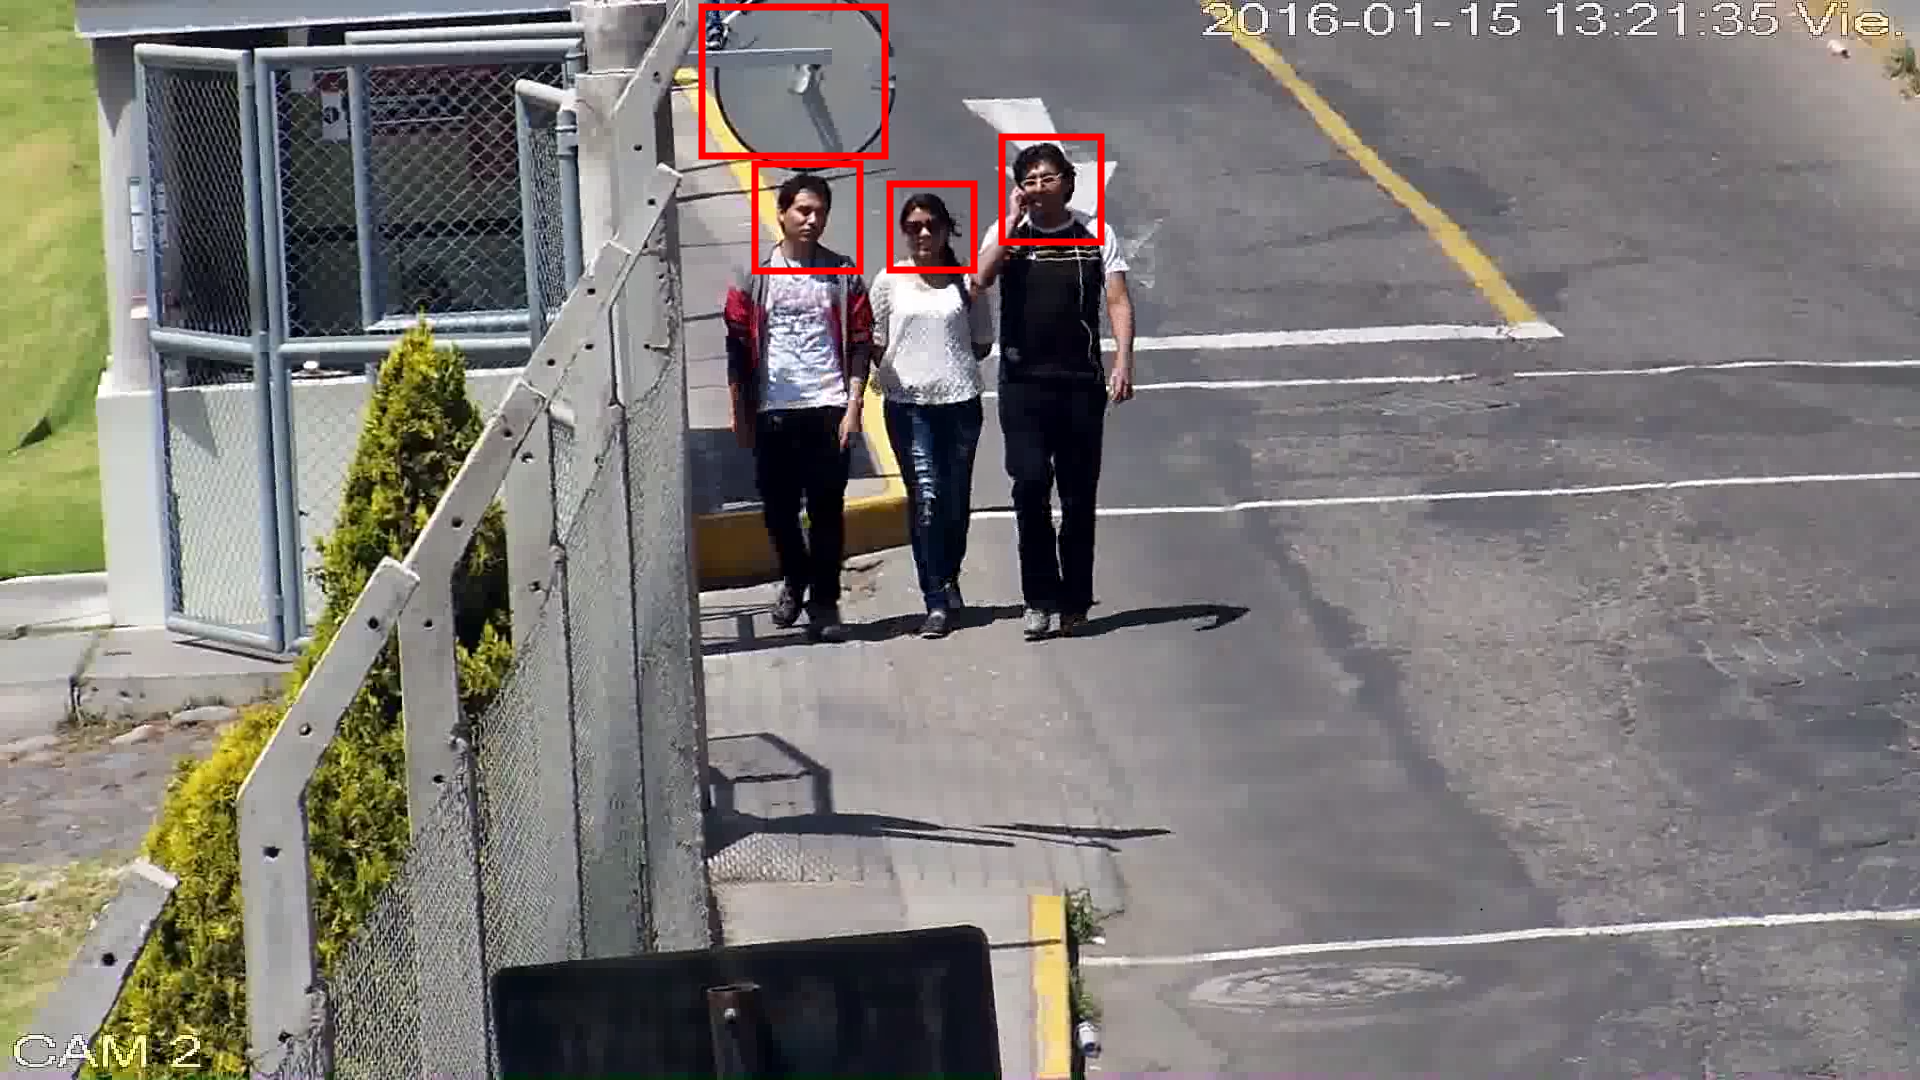
\includegraphics[scale=0.2]{escena_Muestra_error}
\caption{Muestra de  una escena de vídeo vigilancia usando el detector de Viola-Jones}
\label{im:EscenaViola}
\end{figure}

\begin{figure}[h]
\center
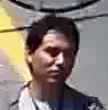
\includegraphics[scale=0.79]{pepe}
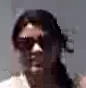
\includegraphics[scale=1]{elian}
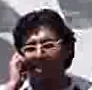
\includegraphics[scale=1]{josimar}
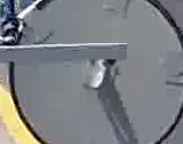
\includegraphics[scale=0.6]{Error}
\caption{Ejemplo de detecciones usando el detector de Viola-Jones, donde la ultima imagen es un falso positivo}
\label{im:EscenaViolaResultados}
\end{figure}

\subsection{Validación con detector de \ac{HOG}}
Para filtrar los falsos positivos que puede entregar el algoritmo de Viola-Jones se propone usar el detector de \ac{HOG} para rostros. %esta elección es motivada por dos razones.

El proceso de detección de rostros usando \ac{HOG} toma una imagen y la trasforma con el descriptor de \ac{HOG} donde se resalta las lineas de contraste y entrega información sobre la gradiente de dicho contraste como se observa en la Figura \ref{im:HOG}

\begin{figure}[h]
\center
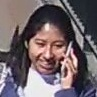
\includegraphics[scale=1.5]{face}
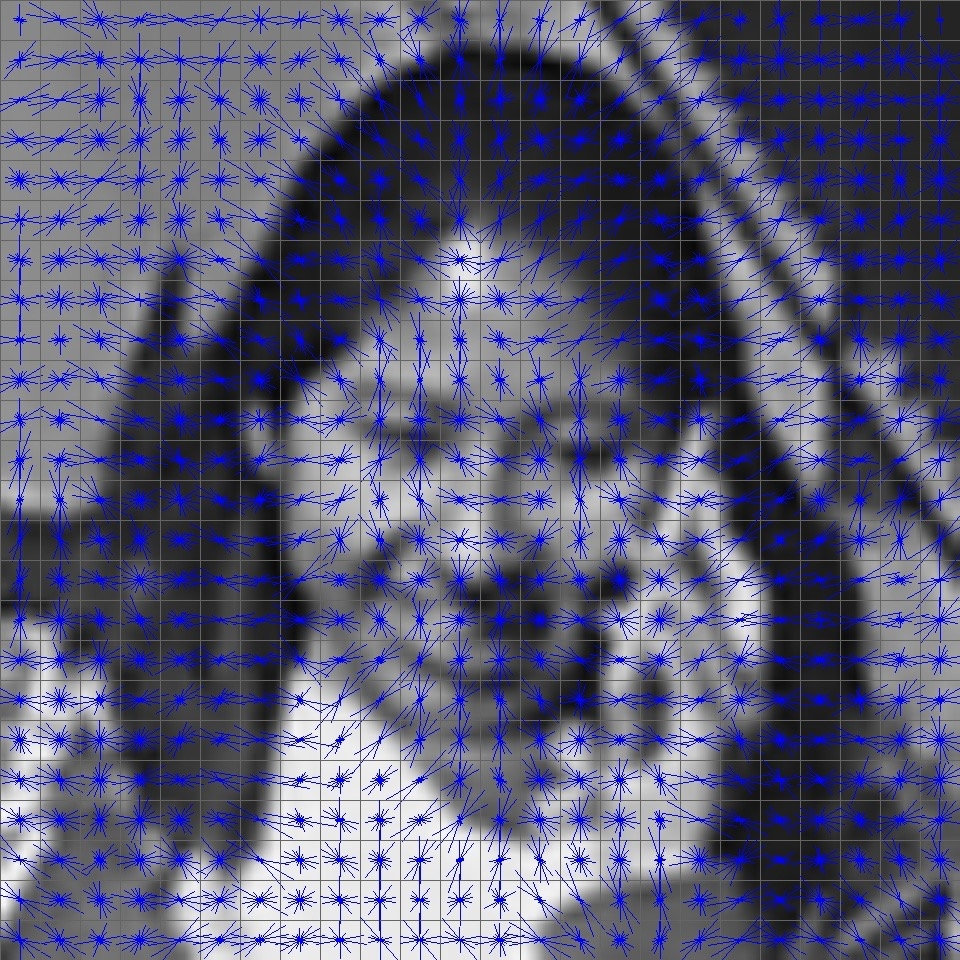
\includegraphics[scale=0.15]{hog}
\caption{Muestra de representación del descriptor de \ac{HOG}(derecha) en una imagen de rostro(izquierda), donde el total de la imagen es transformada a un vector de características.}
\label{im:HOG}
\end{figure}

Para analizar las imágenes representadas por el descriptor de \ac{HOG} se utiliza un \ac{SVM} que se ha sido entrenado con ejemplos positivos y negativos de rostros, con ello se valida los resultados entregados por Viola-Jones vistos en la Figura \ref{im:EscenaViolaResultados}.

Las información proporcionada por el descriptor de \ac{HOG} es entregada a la siguiente parte del proceso como la primera estimación de puntos fiduciales.

%La segunda es que en la continuación de la linea de proceso esta un detector de puntos fiduciales para los rostro detectados, el cual necesita una primera estimación de puntos como lo menciona \cite{baltrusaitis2013constrained} y la representación en el descriptor de \ac{HOG} cumple este trabajo.

\section{Detector de puntos fiduciales}
A partir de los resultados obtenidos por el proceso de detección y validación se tiene una imagen la cual es utilizado en el calculo de los puntos fiduciales mediante \acf{CLNF}.

El método de \ac{EBGM} se basa en modelos de rostros, esto modelos son los puntos encontrados manualmente (ojos, nariz, boca, etc) como se observa en la Figura \ref{im:22Landmark}, dichos modelos se obtienen de un conjunto variado de rostros, a partir de los cuales se calcula un modelo promedio, que se utiliza como estimación inicial para un nuevo rostro mediante el alineamiento con el conjunto de modelos en base a las coordenadas de los ojos 

Se extraen características de la nueva imagen en base a las coordenadas de puntos del modelo promedio, y por cada punto se realiza una comparación del Gabor Wavelet en la nueva imagen con su equivalente en todos los modelos, hasta encontrar el punto del modelo con mayor similitud con ello se obtiene la estimación final de los puntos. Este es un proceso de fundamental ya que una mala estimación de los puntos repercute en el proceso de reconocimiento.

Se propone el uso de \acf{CLNF} en reemplazo de todo el proceso detección de puntos usado en \ac{EBGM}, debido a que \ac{CLNF} es un detector robusto y probado en ambiente no controlados, con una buena tolerancia a variaciones de pose.

\ac{CLNF} recibe el resultado del detector de \ac{HOG} y realiza una estimación de puntos, a partir de ahí se restringe cada punto a un área de vecindad donde se aplica una red neuronal que entrega información espacial sobre cuales son las posiciones que tiene mayor probabilidad de ser el verdadero punto a detectar, el resultado de los puntos detectados es evaluado en conjunto para encontrar la configuración de puntos que resulte mas probable en conjunto, de esta manera se eliminan expresiones y formas de rostro poco probables. Finalmente se entrega las posiciones de 68 puntos en el rostro.

Todo ello permite llevar a \ac{EBGM} a un entorno de vídeo vigilancia sin ayuda de un factor humano, lo que antes no era posible. La totalidad de este proceso se puede apreciar en los algoritmos \ref{alg:Propuesta} y \ref{alg:ImToGrph}.

\section{Pre-procesamiento y normalización de imágenes}\label{scc:PropIluminacion}

Una vez el rostro ha sido detectado, validado y con los puntos fiduciales encontrados, a la imagen del rostro se le aplica una mejora en iluminación a través de ecualización de histograma, transformada de logaritmo y transformada discreta de coseno, presentada en el trabajo de Manjula (\cite{manjulaimage}), siendo la siguiente Ecuación \ref{f_normaliza}:

\begin{equation}
	F(x,y) = c_{1}*DCT + c_{2}*Lg + c_{3}*HE
    \label{f_normaliza}
\end{equation}
Donde $c_{1}, c_{2}, c_{3}$ son valores tipo peso para equilibrar el efecto de las técnicas usadas, sus valores son de 0.3 , 0.2 y 0.5 respectivamente, donde estos valores fueron calculados después de permutar todos las combinaciones posibles. El resultado de este proceso puede verse en la Figura \ref{im:Preprocess}.

\begin{figure}[h]
\center
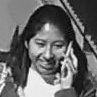
\includegraphics[scale=1.5]{face_original}
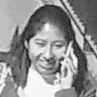
\includegraphics[scale=1.5]{face_pre}
\caption{Muestra del pre-procesamiento aplicado a imágenes, comparando antes y después}
\label{im:Preprocess}
\end{figure}

Junto con ello se aplica el proceso normalización en tamaño que usa \ac{EBGM} que mueve las coordenadas de los ojos a coordenadas pre establecidas $(52, 64)$ y $(76, 64)$ y cambia su resolución a un tamaño de $128 \times 128$ a través de una matriz de transformación de  perspectiva, donde se incluye un borde de 30 pixeles, por lo que el tamaño efectivo de rostros en la imagen final es aproximadamente 90 pixeles de ancho.

Se mantiene la resolución del algoritmo original de \cite{bolme2003elastic} debido a que es necesario aproximarse a resoluciones de rostros que se pueden encontrar en vídeos de vigilancia.
Este proceso y el descrito en la siguiente sección puede ser observado en el algoritmo \ref{alg:ImToGrph}

\begin{algorithm}
\SetKwFunction{ImToGrph}{\textit{ConvertirImagenGrafo}}
\ImToGrph{\var{image},\var{faceLandmark},\var{mask},\var{filter}}\;
{
\var{source} $\gets$ extraer coordenadas de ojos de \var{faceLandmark}\;
\var{M} $\gets$ Calcular una matriz de transformación de perspectiva para que las coordenadas de \var{source} correspondan a las coordenadas $(52,64)$ y $(76,64)$,  y el tamaño de la imagen sea cambiado a $128 \times 128$\;
\var{geo} $\gets$ aplicar la matriz de transformación \var{M} a \var{image}\;
\var{geo} $\gets$ aplicar mejora de iluminación\;
\var{faceLandmark} $\gets$ usar \var{filter} para filtrar puntos fiduciales de interés\;
\var{graph} $\gets$ generar grafo de puntos a partir de \var{faceLandmark}\;
\var{graph} $\gets$ aplicar la matriz de transformación \var{M} a coordenadas de vértices de \var{graph}\;
\ForEach{\var{vertice} en \var{graph}}
{
	extraer Gabor Jet de las coordenadas del vértice usando el conjunto de mascaras de Gabor incluidas en \var{mask}\;
    Almacenar Gabor Jet dentro de \var{graph} en relación con \var{vertice}\;
}
\Return \var{graph}\;
}

\caption{Función para convertir una imagen a Face Graph}
\label{alg:ImToGrph}
\end{algorithm}

\section{Filtro y reajuste de puntos detectados}
Mientras que \ac{EBGM} propuesto en \cite{bolme2003elastic} funciona con 25 puntos fiduciales, de los cuales 3 de ellos se refieren al cabello, usando el detector de puntos \ac{CLNF} se determina 68 puntos de los cuales muchos son cercanos unos a otros por lo que extraer características en todos ellos resulta redundante, ademas ninguno de los puntos obtenidos a través de \ac{CLNF} corresponden a los 3 puntos que se refieren al cabello.

\begin{figure}[h]
\center
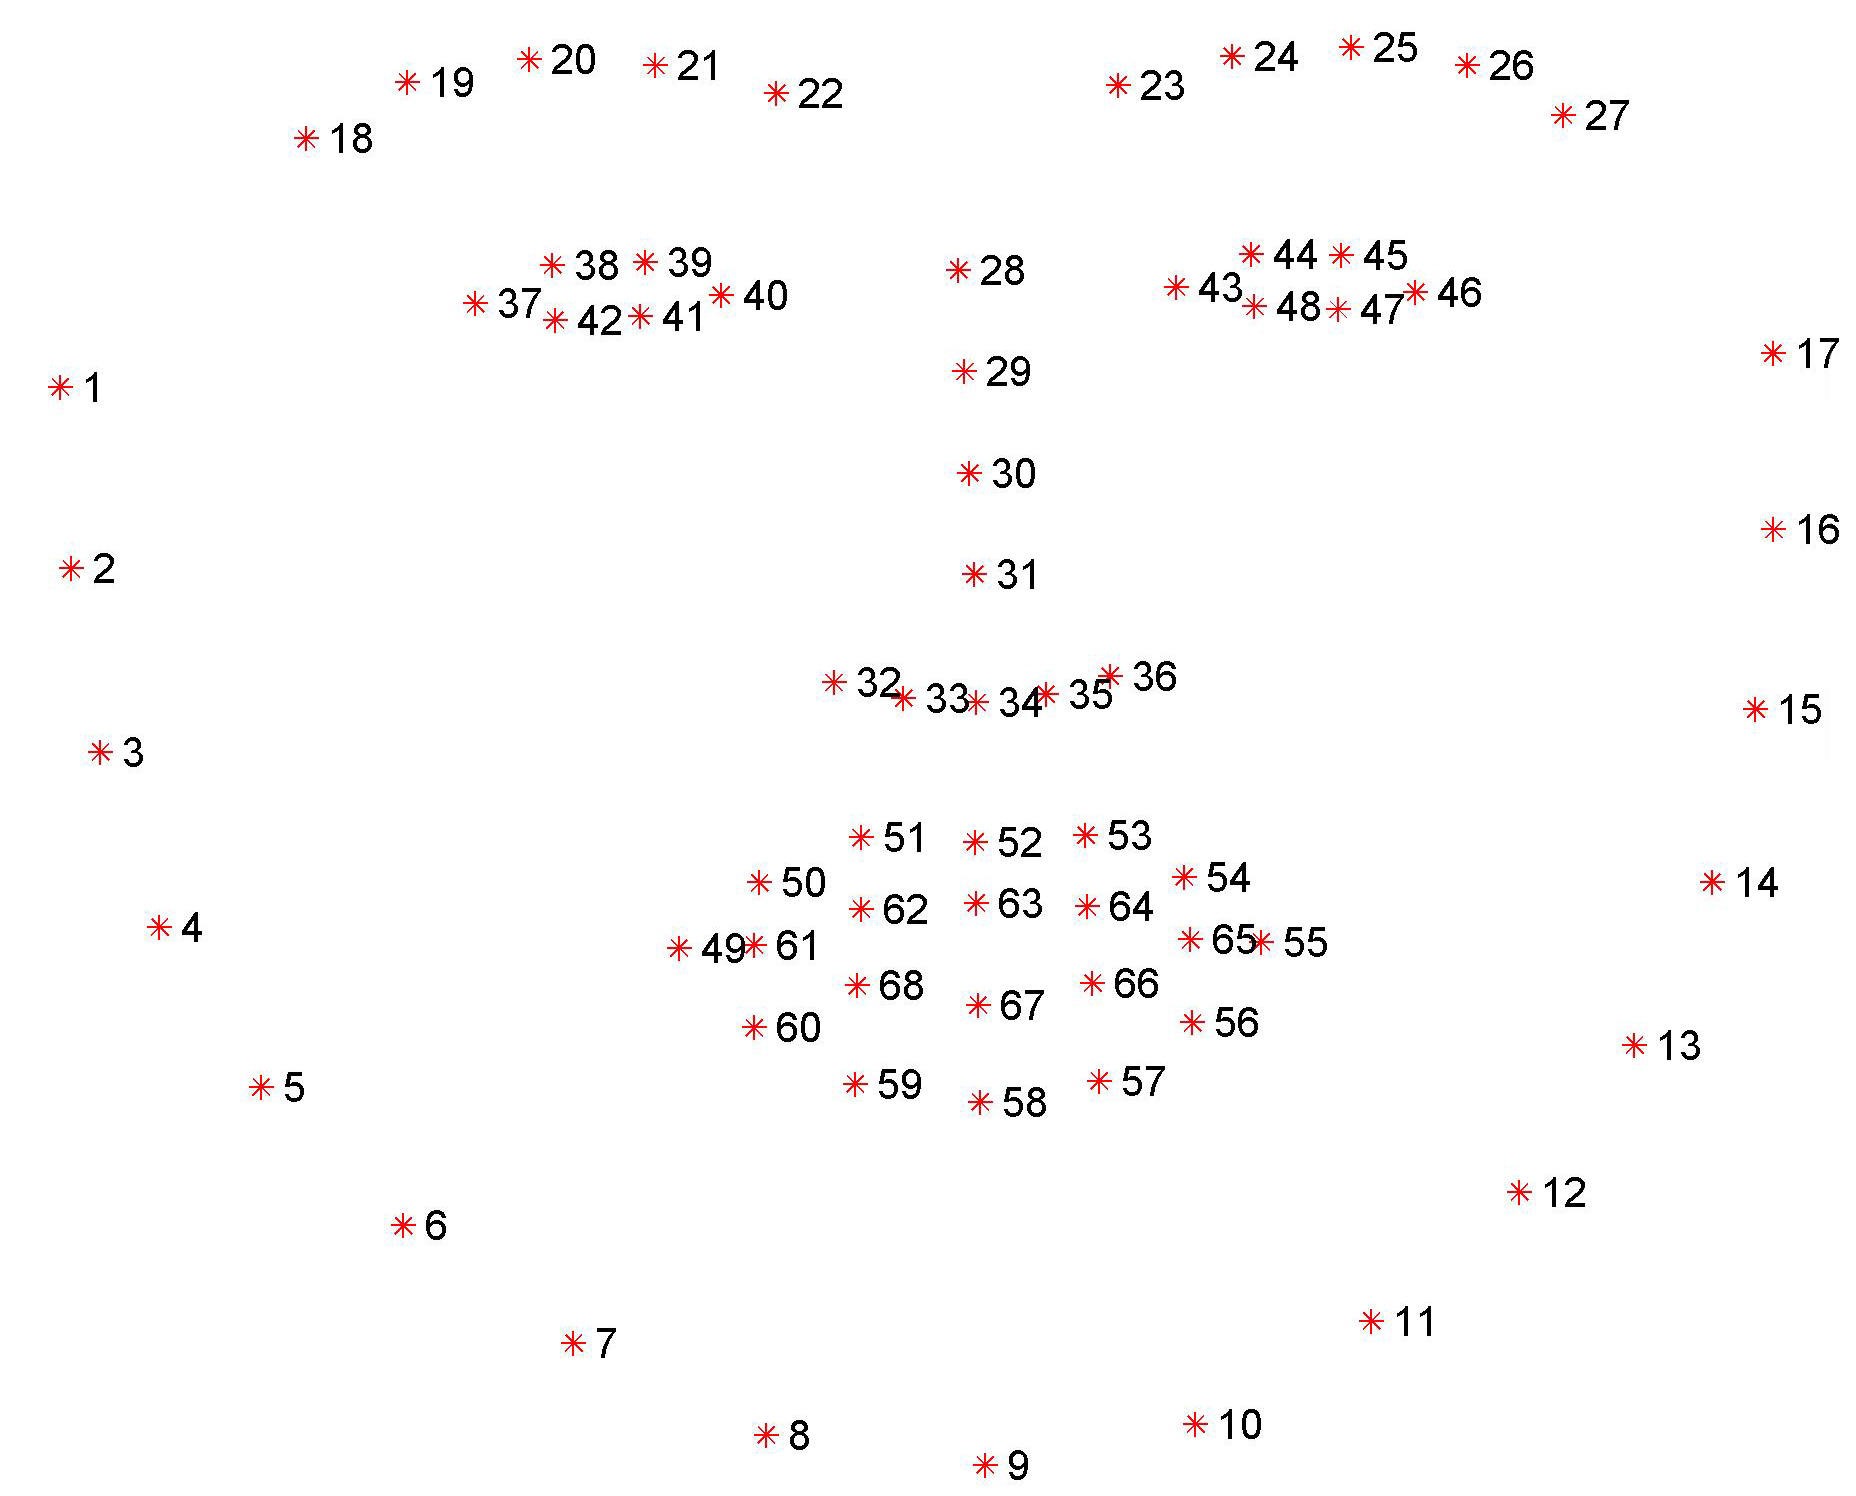
\includegraphics[scale=0.12]{landmarkPoints}
\caption{Puntos fiduciales entregados por \ac{CLNF}, extraído del proyecto ``Open Face''}
\label{im:68Landmark}
\end{figure}

Por lo que es necesario un filtrado de puntos para realizar una correspondencia con los puntos con los que trabaja \ac{EBGM}, por ello se deja de trabajar con estos 3 puntos fiduciales, siendo la cantidad efectiva de trabajo reducida de 25 a 22 puntos, Figura \ref{im:22Landmark}.

\begin{figure}[h]
\center
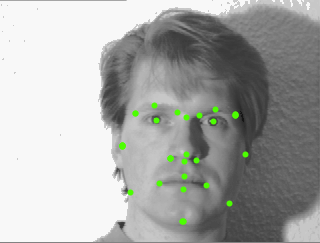
\includegraphics[scale=0.9]{FiltroDespues}
\caption{Puntos fiduciales después del proceso de filtrado}
\label{im:22Landmark}
\end{figure}

Después del filtrado toda la información se completa a un grafo y se aplica una transformada de perspectiva obtenida en el paso anterior para que los vértices correspondan a la imagen normalizada y se continua el proceso de extracción de características de \ac{EBGM}.{}

\section{Proceso de \ac{EBGM}}
Después de reemplazar el proceso de localización de puntos, se continua con el proceso de reconocimiento explicado en la Sección \ref{scc::EBGM} el cual se puede entender en el Algoritmo \ref{alg:ImToGrph}. El proceso empiza cuando extraen características de los puntos fiduciales a través de las convoluciones con las mascaras de Gabor, donde el grupo de coeficientes de resultado son almacenados en una estructura tipo grafo.

Finalmente cada imagen representada como un grafo que es comparada con las imágenes de entrenamiento en una comparación una a uno usando las Ecuaciones \ref{FaceGraphSimiFunc} y \ref{GaborJetSimiFunc}, y eligiendo al grafo con el cual posee mayor similitud. Este proceso es descrito en el Algoritmo \ref{alg:RecFaceGrph}.

Una vez obtenido un resultado de reconocimiento este es visualizado mostrado el nombre del sujeto reconocido sobre el área de su rostro detectado.

\begin{algorithm}
\SetKwFunction{RecFaceGrph}{\textit{ReconocerFaceGraph}}
\RecFaceGrph{\var{faceGraph},\var{graphs}, \var{names}}\;
\var{menor} $\gets$ 10\;
\For{\var{i} $\gets$ 0, \var{i}< tamaño de \var{graphs}}
{
	\var{distance} $\gets$ medir similitud entre \var{faceGraph} y \var{$graphs_{[i]}$}\;
    \If{\var{distance}<\var{menor}}
    {
    	\var{name} $\gets$ \var{$names{[i]}$}\;
    }
}
\Return{name}\;
\caption{Función para comparar un Face Graph con el conjunto de Face Graph de entrenamiento}
\label{alg:RecFaceGrph}
\end{algorithm}

\section{Consideraciones finales}
El aporte de la propuesta es todo el \textit{pipeline} donde se ha logrado aplicar \ac{EBGM} para su uso de vídeo vigilancia gracias al uso de una de las ultimas propuestas en una linea de investigación para el reconocimiento de puntos de interés (\ac{CLNF}), donde el detalle de toda la propuesta puede observarse en la Figura \ref{im:PropPipeline}. 

Se resalta el uso de mejoras para la iluminación usando una unión de varios procesos conocidos, así mismo las transformaciones de tamaño sobre el rostro detectado para poder aproximarnos a resoluciones que son comunes en este escenario particular.

Se realizaron varias pruebas para llegar a la propuesta final, muchas de las cuales demuestran las dificultades que presenta en el reconocimiento de rostros en vídeo vigilancia y la imposibilidad de usar algunas técnicas en este contexto

\chapter{Resultados} \label{chap:Resultados}


En este capítulo se muestran los los resultados de investigación de la presente tesis, el presente capítulo se divide en dos partes. La primera parte son las base de datos con las que se ha trabajado, donde las tres primeras fueron utilizadas para las pruebas iniciales de la investigación, para realizar comparativas entre métodos de reconocimiento de rostro y el análisis paramétrico que se realizó después, mientras que la ultima base de datos fue hecha para las pruebas finales de la propuesta, finalizando la primera parte se explica el método de experimentación que se uso para todas las pruebas


La segunda parte muestra varias secciones de resultados como: Comparación de \ac{EBGM} con otros métodos holísticos, Evaluación paramétrica de \ac{EBGM}, Evaluación en el \textit{pipeline} y la pruebas de la propuesta. Las dos primeras secciones se enfocan en \ac{EBGM}, en comparación con otros métodos y el estudio de su funcionamiento a través de una evaluación paramétrica, la tercera sección se enfoca en prueba de modificaciones propuestas al \textit{pipeline} explicado en el Capítulo \ref{chap:Propuesta}, y finalmente las ultimas secciones se dedican a mostrar los resultados finales de la propuesta en imágenes obtenidas de cámaras de seguridad y su aplicación para reconocer imágenes ofuscadas.

\section{Base de datos}
A continuación se menciona una descripción de las bases de datos usadas en las pruebas de este capítulo y una creada a partir de imágenes obtenidas de una cámara de seguridad para la prueba de la propuesta final.
\subsection{AT\&T}
Presentada en \cite{ATT}, cuenta con diez imágenes diferentes por cada uno de los 40 sujetos que componen dicha base de datos. En algunos sujetos, las imágenes fueron tomadas en diferentes momentos , las imágenes presentan variación de la iluminación, de las expresiones faciales (ojos abiertos / cerrados, sonriendo / sin sonreír) y de los detalles faciales ( lentes / sin gafas ) . Todas las imágenes fueron tomadas contra un fondo homogéneo oscuro con los sujetos en posición vertical , frontal (con tolerancia para un cierto movimiento lateral). Se puede observa una muestra de esta base de datos en la Figura \ref{Att}.
\begin{figure}[h]
	\centering
	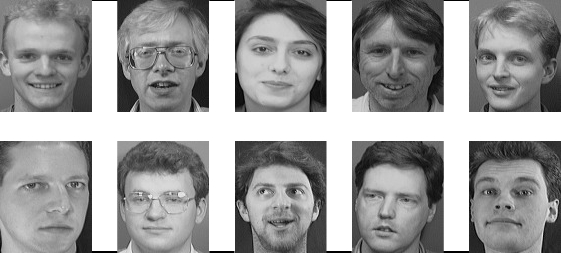
\includegraphics[scale=0.7]{Att}
    \caption{Muestra de imágenes que conforman la base de datos AT\&T}
    \label{Att}
\end{figure}
\subsection{Yale A}
Presentada en \cite{georghiades1997yale}, contiene 165 imágenes en escala de grises en formato GIF de 15 individuos. Hay 11 imágenes por sujeto, una por cada diferente expresión facial o cambio de iluminación: iluminación central , con gafas, feliz, iluminación izquierda, sin gafas ,expresión normal , iluminación derecha , triste , somnoliento , sorprendido , y guiño. Algunas de estas configuraciones pueden apreciarse en la imagen \ref{Yale}
\begin{figure}[h]
	\center
	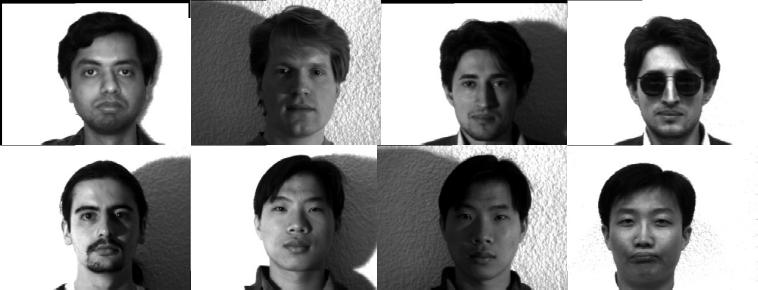
\includegraphics[scale=0.55]{Yale}
    \caption{Muestra de imágenes que conforman la base de datos Yale A}
    \label{Yale}
\end{figure}
\subsection{Georgia Tech}
La base de datos \cite{Georgia} contiene imágenes de 50 personas y se almacena en formato JPEG. Para cada individuo, hay 15 imágenes a color capturadas entre el 06/01/99 y el 15/11/99. La mayoría de las imágenes fueron tomadas en dos sesiones diferentes para tener en cuenta las variaciones en las condiciones de iluminación, la expresión facial y la apariencia. Además de esto, los rostros fueron capturados en diferentes escalas y orientaciones.

Esta base de datos a diferencia de las dos descritas anteriormente es especialmente desafiante por que no es normalizada ni recortada y como se puede observar en la Figura \ref{Georgia} donde el proceso de adquisición es más informal.
\begin{figure}[h]
	\centering
	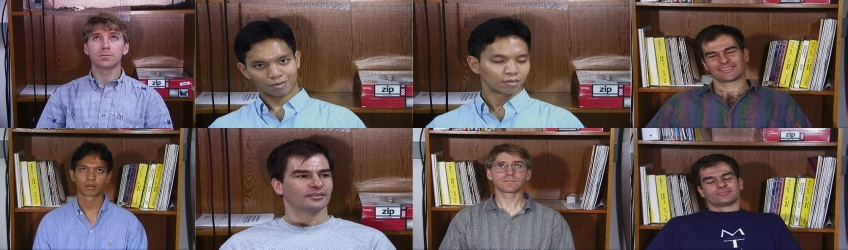
\includegraphics[scale=0.5]{Georgia}
    \caption{Muestra de imágenes que conforman la base de datos Georgia Tech}
    \label{Georgia}
\end{figure}
\subsection{Base de datos generadas a partir de imágenes de cámara de vigilancia}
\label{scc:BDCamara}
Se produjo una base de datos de una cámara de seguridad enfocando la escena vista en la Figura \ref{im:Escena}, con el objetivo de tener un referente de prueba lo mas cercano a la realidad.

La base de datos consiste en 24 sujetos con 8 imágenes cada uno separadas en dos grupos mañana y medio día para probar la variaciones en iluminación, en la Figura \ref{camara} podemos ver una muestra de la base de datos.
\begin{figure}[h]
	\centering
	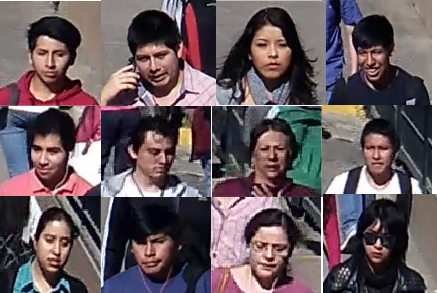
\includegraphics[scale=0.7]{camara}
    \caption{Muestra de imágenes que conforman la base de datos obtenida a partir de una cámara de seguridad}
    \label{camara}
\end{figure}

\section{Método de experimentación}\label{scc:MetdoEx}
Como método de experimentación aplicamos un proceso en cada base de datos que consiste en dividir las imágenes de cada individuo en grupos de 3 a 4 imágenes por sujeto, dependiendo de la base de datos y cada grupo fue usado como entrenamiento mientras el resto es usado como prueba. Este proceso se repite hasta que todos los grupos hayan sido usados como entrenamiento, siendo la cifra final el promedio de los resultados de cada grupo.

\begin{figure}[h]
	\centering
	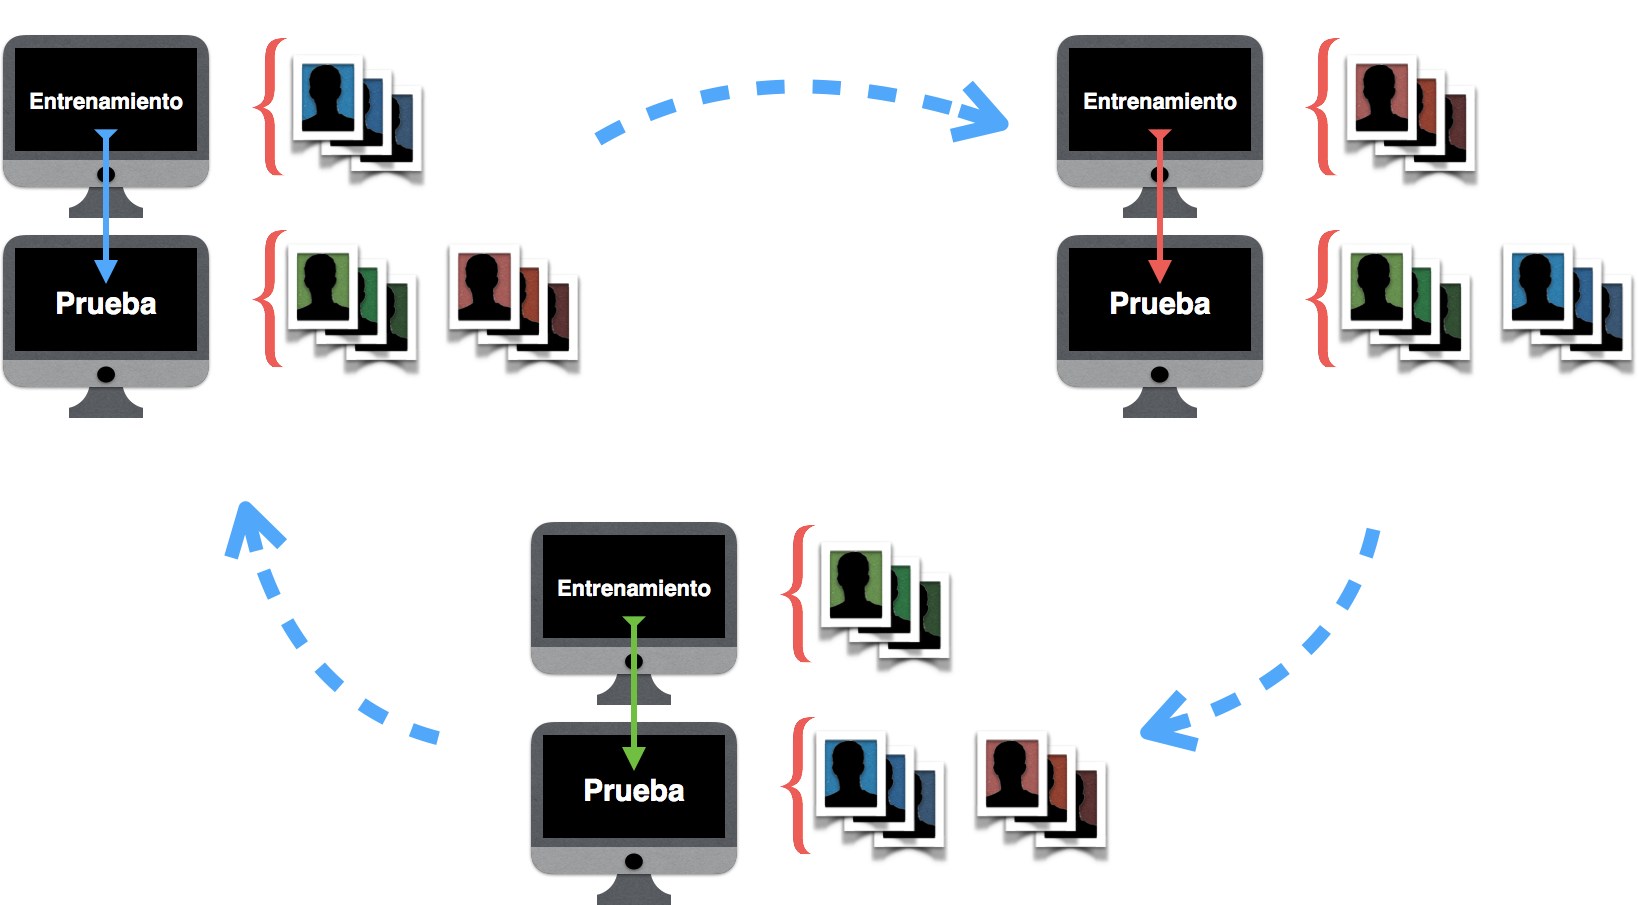
\includegraphics[scale=0.25]{MetodoExp}
    \caption{Muestra del proceso de experimentación, donde las imágenes se dividen por grupos y todos los grupos rotan hasta que todas las combinaciones de prueba y entrenamiento sean probadas}
    \label{metodo}
\end{figure}

La razón para la elección de grupos de entrenamiento tan reducidos es poder acercarnos al escenario de vídeo vigilancia donde en raras ocasiones se cuenta con varias imágenes de los sujetos a identificar.

A continuación se realiza una comparativa del método de reconocimiento usado en la propuesta y otros métodos extraídos del estado del arte.

\section{Comparación de \ac{EBGM} con métodos holísticos}\label{scc:Comparacion}
Se realizó una comparación de \ac{EBGM} con otros métodos de reconocimiento holísticos usados en la literatura como; \ac{PCA}\citep{turk1991eigenfaces}, \ac{KFA}\citep{yang2002kernel} y \ac{LDA}\citep{zhao1999subspace}, todos ellos implementados en matlab por The PhD Toolbox\citep{struc2012phd} para demostrar el rendimiento de estos algoritmos en varias situaciones. Esta comparación se realizo con las tres primeras bases de datos para establecer una diferencia entre el método escogido en la propuesta y otros métodos del estado del arte.

\begin{table}[h]
\centering
\caption{Resultados de aciertos en algoritmos de reconocimiento con bases de datos ATT, Yale A y Georgia}
\label{Tcomparacion}
\begin{tabular}{|l|l|l|l|l}
\cline{1-4}
              & \textbf{ATT/ORL} & \textbf{YALE A} & \textbf{Georgia} &  \\ \cline{1-4}
\textbf{PCA}  & 88.03\%          & 88.18\%         & 76.84\%          &  \\ \cline{1-4}
\textbf{KFA}  & 87.78\%          & 91.72\%         & 75.03\%          &  \\ \cline{1-4}
\textbf{LDA}  & 86.02\%          & 90.21\%         & 75.50\%          &  \\ \cline{1-4}
\textbf{EBGM} & 91.43\%          & 97.94\%         & 77.80\%          &  \\ \cline{1-4}
\end{tabular}
\end{table}
Como se puede apreciar en el Cuadro \ref{Tcomparacion} y mejor aun en la Figura \ref{Fcomparacion}. \ac{EBGM} tiene una tasa de aciertos igual o en algunos casos mejor que los demás métodos comparados. En ninguna de las pruebas realizadas con las tres bases de datos \ac{EBGM} cae por debajo de la tasa de aciertos promedio, esta es una de las razones por la cual se elige a \ac{EBGM} como el método de reconocimiento de rostros en el cual se centra el trabajo de esta tesis.

\begin{figure}[]
\center
	\includegraphics[scale=0.8]{Comparativa}
    \caption{Comparación de \ac{EBGM} con otros algoritmos, la escala empieza en 68,00 para que pueda apreciarse las diferencias entre los métodos}
    \label{Fcomparacion}
\end{figure}

\section{Comparación con otros métodos basados en grafos}
\begin{table}[h]
\caption{Comparación de algoritmos basados en grafos}
\label{Tcomparacion2}
\begin{tabular}{|l|l|c|}
\hline
                         & \textbf{Base de datos}                 & \multicolumn{1}{l|}{\textbf{Resultado reportado}} \\ \hline
Local Graph Matching     & Base de datos propia                   & 98.4\%                                            \\ \hline
\ac{RFG}                 & CMU-PIE frontal illumination variation & 96.1\%                                            \\ \hline
Multiple Facial Features & Cambridge Face Database                & 95.5\%                                            \\ \hline
\sc{EBGM} si cambios     & Yale A                                 & 97.94 \%                                          \\ \hline
Propuesta de iluminación & Yale A                                 & 98.53 \%                                          \\ \hline
\end{tabular}
\end{table}

Se realizo otra comparación de \ac{EBGM} con los métodos basados en grafos explicados en el capitulo \ref{chap:Revision}, como se ve en el Cuadro \ref{Tcomparacion2}, a pesar de que cada trabajo usa una base de dados diferente, se puede observar que que los métodos basados en grafos tiende a un mejor desempeño si los comparamos con los métodos holistícos vistos en el Cuadro \ref{Tcomparacion}, por ello se decide usar \ac{EBGM} como método base para nuestro trabajo, al ser un método bien conocido en el estado del arte.

\section{Evaluación paramétrica de \ac{EBGM}}

El método elegido para el proceso de reconocimiento de rostros es \ac{EBGM}, este ha sido elegido por sus resultado en la comparativa realizada en la Sección \ref{scc:Comparacion}, también por ser un método que es considerado biométrico por lo expuesto en el Capítulo \ref{chap:Conceptos}.

Parte de las contribuciones de este trabajo de tesis consiste en una evaluación de parámetros de \ac{EBGM} para poder incrementar la tasa de aciertos, entiéndase como tasa de acierto al porcentaje respecto a los verdaderos positivos. Finalmente probar el resultado en un ambiente de vídeo vigilancia.

\begin{figure}[h]
\center
	\includegraphics[scale=0.65]{EBGMproccess}
    \caption{Curso de procesos que forman parte del reconocimiento de rostros en \ac{EBGM}}
    \label{im:parametos}
\end{figure}

Se puede observar el curso normal de \ac{EBGM} en la Figura \ref{im:parametos}, y las evaluaciones que se plantean son las siguientes:

\subsection{Incrementar la cantidad de modelos}
En el trabajo de \cite{bolme2003elastic} se usa 70 modelos de rostros de la base de datos FERET gray, el numero de modelos es el mismo que se usa en el trabajo de \cite{wiskott1997face} al que hace referencia.

Para la creación de los modelos se usó la nueva versión de FERET llamada FERET COLOR y se ha elegido nuevas imágenes aleatoriamente para extraer manualmente las coordenadas de los puntos fiduciales, así mismo se ha incrementado el numero de modelos a 150 con el fin de probar si dicho incremento tiene una relación directa con la tasa de aciertos.

\begin{table}[h]
\centering
\caption{Resultado aciertos con incremento de modelos en \ac{EBGM}}
\label{ta:ModelInc}
\begin{tabular}{|c|c|c|c|}
\hline 
                     & \textbf{AT\&T/ORL} & \textbf{Yale A} & \textbf{Georgia} \\ \hline
\textbf{\ac{EBGM} original}  & 91.43\%            & 97.94\%         & 77.80\%          \\ \hline
\textbf{150 Modelos}         & 91.43\%            & 98.21\%         & 78.73\%          \\ \hline
\end{tabular}
\end{table}

Como se puede observar en el Cuadro \ref{ta:ModelInc} existe una mejora en los aciertos, no obstante un incremento en el numero de modelos modelos no implica una mejora proporcional en la tasa de aciertos, lo cual indica que existe un punto en que la cantidad de modelos es suficiente para realizar una estimación precisa.

\subsection{Modificar la función de similitud} 
Usando como base el trabajo de \cite{bolme2003elastic}, en este trabajo se tiene como parte de sus conclusiones y recomendaciones la modificación de la función de similitud con la que se compara los Face Graph que son las representaciones de un rostros en dicho algoritmo.

La modificación que se sugiere investigar es la de añadir pesos a cada punto fiducial que se compara, ya que se puede concluir que no todos los puntos de un rostros son igualmente importantes para realizar un reconocimiento. 

Un ejemplo, es que los puntos del contorno del rostro o el cabello pueden ser menos importantes que los puntos de los ojos o la nariz, así que se añade un vector de pesos a la función de similitud descrita en las Ecuaciones \ref{FaceGraphSimiFunc} y \ref{GaborJetSimiFunc}, probamos varias combinaciones empíricas bajo el concepto que la información con mayor relevancia se encuentra en la boca, nariz y ojos .
\begin{equation}
\label{FaceGraphSimiFuncW}
L_{jet}(G,G',W)=\frac{1}{N}\sum_{i=0}^{N}S(J_{i},J'_{i},w_{i})
\end{equation}
\begin{equation}
\label{GaborJetSimiFuncW}
S(J,J',w)=w*\frac{\sum_{j=1}^{N}a_j a'_jcos(\phi_j-\phi'_j)}{\sqrt{\sum_{j=1}^{N}a_j^2 \sum_{j=1}^{N}{a'}_j^2}}
\end{equation}

En las Ecuaciones \ref{FaceGraphSimiFuncW} y \ref{GaborJetSimiFuncW} podemos observar la adición de un vector $W$ de tamaño $N$ con elementos $w$, lo que permite dar una valoración diferente a cada punto fiducial.

\begin{table}[h]
\centering
\caption{Tabla de distribución de pesos propuesta, donde se distribuyen los 25 puntos fiduciales en áreas y a cada una asignadole pesos representados en porcentajes. La configuración 1 le resta importancia la los bordes del rostros, la configuración 2 resalta la importancia de los ojos y el puente de la nariz, y la configuración 3 se se concentra en el centro del rostro incluyendo nariz y boca}
\label{ta:distPuntos}
\begin{tabular}{|l|c|c|c|c|}
\hline
\textbf{Área}                      & \multicolumn{1}{l|}{\textbf{Nro puntos}} & \multicolumn{1}{l|}{\textbf{Conf. 1}} & \multicolumn{1}{l|}{\textbf{Conf. 2}} & \multicolumn{1}{l|}{\textbf{Conf. 3}} \\ \hline
\textbf{Ojos y puente de la nariz} & 3                                        & 20\%                                  & 50\%                                  & 15\%                                  \\ \hline
\textbf{Cejas}                     & 6                                        & 20\%                                  & 10\%                                  & 15\%                                  \\ \hline
\textbf{Nariz}                     & 4                                        & 20\%                                  & 20\%                                  & 20\%                                  \\ \hline
\textbf{Boca}                      & 4                                        & 20\%                                  & 10\%                                  & 25\%                                  \\ \hline
\textbf{Bordes de la cabeza}       & 5                                        & 10\%                                  & 5\%                                   & 5\%                                   \\ \hline
\textbf{Barbilla y quijada}        & 3                                        & 10\%                                  & 5\%                                   & 20\%                                  \\ \hline
\end{tabular}
\end{table}

En el Cuadro \ref{ta:distPuntos} se observa la agrupaciones que se realizan a los puntos fiduciales y las distribuciones mostradas como porcentajes, donde se le da importancia a áreas que se ubican en el centro del rostro, en el Cuadro \ref{ta:Pesos} se puede ver su correspondencia en valores numéricos para la conformación del vector $W$ usado en la Ecuación \ref{FaceGraphSimiFuncW}.

\begin{table}[h]
\centering
\caption{Valores del vector W de pesos derivado del Cuadro \ref{ta:distPuntos}, donde los valores por área representados a través de porcentajes son transformados a números así el valor de 20\% para los ojos y el puente de la nariz en la configuración 1, valen 0.07 en cada ojo y 0.06 para el puente dando como resultado 0.2 el mismo calculo se produce para el resto de áreas y configuraciones.}
\label{ta:Pesos}
\resizebox{\textwidth}{!}{
\begin{tabular}{|l|c|c|c|}
\hline
\textbf{Puntos Fiduciales}                    & \multicolumn{1}{l|}{\textbf{1ra Config}} & \multicolumn{1}{l|}{\textbf{2da Config}} & \multicolumn{1}{l|}{\textbf{3ra Config}} \\ \hline
\textbf{ojo izquierdo}                         & 0.07                                      & 0.07                                     & 0.05                                                                         \\ \hline
\textbf{ojo derecho}                           & 0.07                                      & 0.07                                     & 0.05                                                                         \\ \hline
\textbf{puente de la nariz}                    & 0.06                                      & 0.07                                     & 0.05                                                                         \\ \hline
\textbf{pico ceja derecha}                     & 0.03                                      & 0.025                                    & 0.025                                                                        \\ \hline
\textbf{pico ceja izquierda}                   & 0.03                                      & 0.025                                    & 0.025                                                                        \\ \hline
\textbf{interior ceja derecha}                 & 0.04                                      & 0.025                                    & 0.025                                                                        \\ \hline
\textbf{interior ceja izquierda}               & 0.04                                      & 0.025                                    & 0.025                                                                        \\ \hline
\textbf{exterior ceja derecha}                 & 0.03                                      & 0.025                                    & 0.025                                                                        \\ \hline
\textbf{exterior ceja derecha}                 & 0.03                                      & 0.025                                    & 0.025                                                                        \\ \hline
\textbf{punta de la nariz}                     & 0.05                                      & 0.08                                     & 0.05                                                                         \\ \hline
\textbf{centro base de la nariz}               & 0.05                                      & 0.07                                     & 0.05                                                                         \\ \hline
\textbf{base derecha de la nariz}              & 0.05                                      & 0.07                                     & 0.05                                                                         \\ \hline
\textbf{base izquierda de la nariz}            & 0.05                                      & 0.07                                     & 0.05                                                                         \\ \hline
\textbf{parte central superior de la boca}     & 0.05                                      & 0.0375                                   & 0.0625                                                                       \\ \hline
\textbf{parte central inferior de la boca}     & 0.05                                      & 0.0375                                   & 0.0625                                                                       \\ \hline
\textbf{esquina izquierda de la boca}          & 0.05                                      & 0.0375                                   & 0.0625                                                                       \\ \hline
\textbf{esquina derecha de la boca}            & 0.05                                      & 0.0375                                   & 0.0625                                                                       \\ \hline
\textbf{parte central superior de la cabeza}   & 0.02                                      & 0.02                                     & 0.01                                                                         \\ \hline
\textbf{parte izquierda superior de la cabeza} & 0.02                                      & 0.02                                     & 0.01                                                                         \\ \hline
\textbf{parte derecha superior de la cabeza}   & 0.02                                      & 0.02                                     & 0.01                                                                         \\ \hline
\textbf{borde izquierdo de la cara}            & 0.02                                      & 0.02                                     & 0.01                                                                         \\ \hline
\textbf{borde derecho de la cara}              & 0.02                                      & 0.02                                     & 0.01                                                                         \\ \hline
\textbf{centro de la barbilla}                 & 0.04                                      & 0.04                                     & 0.06                                                                         \\ \hline
\textbf{parte izquierda de la quijada}         & 0.03                                      & 0.03                                     & 0.07                                                                         \\ \hline
\textbf{parte derecha de la quijada}           & 0.03                                      & 0.03                                     & 0.07                                                                         \\ \hline
\end{tabular}
}
\end{table}

En el Cuadro \ref{ta:ResultadosPesos} se observan los resultados de las configuraciones propuestas para modificación la función de similitud de \ac{EBGM}, en la Figura \ref{im:ResultadoPesos} vemos que la primera configuración ofrece una mejora de 2\% en la base de datos Georgia y mantiene el rendimiento en el resto de las base de datos. Esta configuración distribuye los pesos uniformemente a todas las áreas del centro del rostro en detrimento de los bordes como son la barbilla y la quijada.

\begin{table}[h]
\centering
\caption{Resultados de adición de pesos \ac{EBGM}}
\label{ta:ResultadosPesos}
\begin{tabular}{|l|l|l|l|}
\hline
\textbf{Propuestas}                     & \textbf{AT\& T} & \textbf{Yale} & \textbf{Georgia} \\ \hline
\textbf{\ac{EBGM} sin cambios}             & 91.43\%      & 97.94\%       & 77.80\%          \\ \hline
\textbf{Primera configuración de pesos} & 91.67\%      & 97.58\%       & 80.43\%          \\ \hline
\textbf{Segunda configuración de pesos} & 91.15\%      & 97.86\%       & 79.40\%          \\ \hline
\textbf{Tercera configuración de pesos} & 90.16\%      & 96.71\%       & 76.70\%          \\ \hline
\end{tabular}
\end{table}

En el resto de las configuraciones se observan resultados variados donde se presentan mejoras del 1\% en las tres bases de datos con excepción de la tercera configuración donde se le resta importancia a los ojos, para probar la importancia del centro del rostro como fuente de información.

\begin{figure}[ht]
	\centering
	\includegraphics[scale=0.6]{ResultadoPesos}
    \caption{Comparación entre las configuraciones propuestas para los pesos en la función de similitud de \ac{EBGM}}
    \label{im:ResultadoPesos}
\end{figure}

\subsection{Incrementar la cantidad de imágenes de entrenamiento a través de transformaciones de perspectiva} 
Una de las restricciones más grandes que conlleva el reconocimiento de rostros en vídeo vigilancia, es el hecho de que en muchos sistema de vigilancia no se cuenta con varias imágenes por sujeto para realizar un entrenamiento adecuado. En muchos casos solo se cuenta con una imagen, ya puede ser de un carnet o una fotografía de perfil y en varios casos son imágenes que no están al día. 

Por ello se plantea crear más imágenes de entrenamiento a partir de una sola imagen a través de varias transformaciones de perspectiva para probar si con una imagen frontal podemos crear imágenes de rostros que parezcan mirar a otros sentidos y así poder aumentar el numero de entrenamiento y con ello el porcentaje de aciertos.

\begin{figure}[h]
	\centering
	\includegraphics[scale=1]{trans_original}
    \caption{Imagen de entrenamiento original}
\end{figure}

Para lograr ello generamos una matriz de transformación en 3D donde realizamos las rotaciones necesarias en el eje Z para crear la ilusión de cambio de pose, después realizamos un conversión a un matriz de transformación 2D y la aplicamos a la imagen. Los resultados de dicha transformación se pueden apreciar en la Figura \ref{im:Transformacion}.

\begin{figure}[h]
	\centering
	\includegraphics[scale=0.6]{trans1}
    \includegraphics[scale=0.6]{trans2}
    \includegraphics[scale=0.6]{trans3}
    \caption{Resultados de las transformaciones de perspectiva}
    \label{im:Transformacion}
\end{figure}

En las pruebas hechas a \ac{EBGM}, no se muestra ningún cambio y en los resultados experimentales. el uso de las trasformaciones no ayudan a mejorar la tasa de aciertos pero tampoco la empeoran. En ningún caso una imagen generada por la transformación de perspectiva es elegida como resultado del proceso de reconocimiento.

\subsection{Ajuste de tamaño a máscaras de Gabor}
La Ecuación \ref{GaborWavelet} define el Gabor Wavelet que se usa para crear máscaras de Gabor. Con esta ecuación podemos crear varios tamaños de máscaras, donde la configuración original es $N \in \left\{25, 37, 51, 71, 101 \right\}$. En conjunción al resto de parámetros explicados en la Sección \ref{sscc:GaborWavelet} se obtienen 80 configuraciones de Gabor Wavelet y siendo efectivas 40 máscaras por punto fiducial, debido a que existe una mascara que extrae la parte imaginara y otra la parte real del Wavelet.

La propuesta de modificación plantea el cambio del tamaño de las Gabor Wavelet, debido a que tamaños de 71 y 101 son demasiado grandes teniendo en cuenta que la imagen a convolucionar es de $128 \times 128$ y el tamaño efectivo del rostro es aun menor siendo los tamaños propuestos $N \in \left\{13, 19, 25, 35, 51 \right\}$ los resultados pueden observarse en el Cuadro

\begin{table}[h]
\centering
\caption{Resultados de pruebas en tamaños de mascaras de Gabor }
\label{ta:ResultadosMascaras}
\begin{tabular}{|l|c|c|c|}
\hline
\textbf{}                                         & \multicolumn{1}{l|}{\textbf{AT\&T}} & \multicolumn{1}{l|}{\textbf{Yale}} & \multicolumn{1}{l|}{\textbf{Georgia}} \\ \hline
\textbf{Sin cambios}                              & 91.43\%                             & 97.94\%                            & 77.80\%                               \\ \hline
\textbf{Propuesta de mascaras de Gabor} & 93.18\%                             & 97.58\%                            & 79.43\%                               \\ \hline
\end{tabular}
\end{table}

Se observa mejoras de 2\% en las bases de datos AT\&T y Georgia, mientras que en Yale mantiene el porcentaje de aciertos. Un efecto a parte de la mejora en el acierto es que al tener un tamaño de mascaras menor el tiempo en convoluciones también se disminuye.
\section{Evaluaciones en el \textit{pipeline} de reconocimiento}
Como parte de la propuesta es necesario encontrar un método de validación para confirmar las detecciones de rostros proporcionadas por el algoritmo de Viola-Jones, en esta sección se muestran resultados sobre las opciones exploradas para afrontar este problema

\subsection{Evaluación del detector de Viola-Jones para detección de ojos}\label{sscc:DectOjos}
Para poder usar \ac{EBGM} tal como se presenta en \cite{bolme2003elastic} y \cite{wiskott1997face} en un \textit{pipeline} de vídeo vigilancia es necesario proporcionar las coordenadas de los ojos.

Para ello se necesita establecer un proceso o una forma de detección de ojos con una gran robustez, ya que un error en la detección de ojos resulta en un fallo de todo el proceso de reconocimiento

Como parte de este trabajo se realizo pruebas de un detector de Viola-Jones entrenado para detectar ojos como opción para encontrar coordenadas de ojos y empezar el proceso de reconocimiento. Para ello se probó el Algoritmo \ref{alg:DetecOjos}.

\begin{algorithm}
\var{face} $\gets$ rostro detectado por un detector de rostros\;
\var{eyes} $\gets$ lista de ojos detectados en \var{face}\;
\For{\var{i}  $\gets$ 0, \var{i}< tamaño de \var{eyes}}
{
    \If{la posición de \var{$eyes_[i]$} no se encuentra en la región superior central de \var{face}}
    {
    	descartar \var{$eyes_[i]$} de \var{eyes}\;
    }
}
\var{region} $\gets$ dividir la región superior central de \var{face} en cuatro pares de sub-regiones \;
agrupar todos los ojos detectados en \var{eyes} segun su posicion dentro de \var{region}\;
\For{cada \var{region}}
{
	calcular el punto promedio a partir todos los \textit{eyes} en  \textit{region}\;
}
Elegir el par de puntos perteneciente al par de \textit{region} según la mayor cantidad de puntos que posee\;
\caption{Proceso de detección de ojos en rostro para \ac{EBGM}}
\label{alg:DetecOjos}
\end{algorithm}

\begin{figure}[h]
	\centering
	\includegraphics[scale=0.35]{OjosViolaJones}
    \caption{Ejemplo de proceso de detección de ojos Nro 1}
    \label{im:HaarOjos1}
\end{figure}

Como se puede observar en las Figuras \ref{im:HaarOjos1} y \ref{im:HaarOjos2} el proceso que propone el algoritmo \ref{alg:DetecOjos} ofrece resultados variados, el motivo de ello es la naturaleza del algoritmo de Viola-Jones, los ojos poseen menos variaciones de sombras si se lo compara con un rostro y ademas el calculo imagen integral es dependiente a la iluminación de la imagen.

\begin{figure}[h]
	\centering
    \includegraphics[scale=0.35]{OjosViolaJones2}
    \caption{Ejemplo de proceso de detección de ojos Nro 2}
    \label{im:HaarOjos2}
\end{figure}

\subsection{Validación de detecciones mediante color de piel}
Se probó como método de validación de las detecciones proporcionadas por Viola-Jones, el uso de un método de confirmación a través de detectores de color de piel sel cual se detalla en el algoritmo \ref{alg:ColorPiel}.

\begin{algorithm}[h]
\var{face} $\gets$ rostro detectado\;
\var{imageHSV} $\gets$ convertir \var{face} a espacio de color HSV\;
\var{binaryImage} $\gets$ binarizar imagen bajo un threshold de 70 en el canal Hue de \var{imageHSV}\;
\var{count} $\gets$ contar pixeles blancos de \var{binaryImage}\;
\eIf{\var{count}> al 50\% del total de pixeles de \var{face}}
{
	validar \var{face} como imagen de un rostros\;
}
{
	descartar \var{face} como imagen de un rostros\;
}
\caption{Validación de detecciones a través de color de piel}
\label{alg:ColorPiel}
\end{algorithm}

Realizando pruebas en videos como se puede ver en la figura \ref{im:skinDetector}, se observan problemas de validación debido a que los colores de piel están entre 0 y 70 en canal Hue, pero también están otros colores como el naranja se encuentran en ese mismo rango debido a la variación de los otros dos canales. Así mismo todos los colores de piel humana no se encuentran agrupados en una sola región del rango de todo el canal, sobre todo colores oscuros de piel.
\begin{figure}[h]
	\centering
    \includegraphics[scale=0.2]{SkinDetector}
    \caption{Ejemplo de falsas validaciones en colores cercanos al rojo y naranja.}
    \label{im:skinDetector}
\end{figure}

\subsection{Mejora de la iluminación en el pre-procesamiento} 
\ac{EBGM} tiene un pre-procesamiento para normalizar la información introducida, pero este pre-procesamiento solo consiste en una normalización de los valores de los pixeles de las imágenes, una transformación de tamaño a un estándar de $128 \times 128$ y la añadidura de bordes de 30 pixeles a la imagen. 
El uso de esto bordes se justifican en el trabajo de \cite{bolme2003elastic} como una forma de ayudar a que su ajuste de puntos fiduciales converja en el centro de la imagen y no tienda a alejarse a los borde, y como método para filtrar la información del fondo que pueda quedar después de la transformación de perspectiva aplicada.

Para cubrir esta falta de una mejora en iluminación, la propuesta explicada en la Sección \ref{scc:PropIluminacion} implica la modificación de este proceso para así volverlo más robusto a cambios de luz.

\begin{table}[h]
\centering
\caption{Resultados de la propuesta de iluminación}
\label{ta:ResultadosIluminacion}
\begin{tabular}{|l|c|c|c|}
\hline
\textbf{}                           & \multicolumn{1}{l|}{\textbf{AT\&T}} & \multicolumn{1}{l|}{\textbf{Yale}} & \multicolumn{1}{l|}{\textbf{Georgia}} \\ \hline
\textbf{\ac{EBGM} sin cambios}                & 91.43\%                             & 97.94\%                            & 77.80\%                               \\ \hline
\textbf{Ecualización de histograma} & 92.78\%                             & 96.67\%                            & 79.13\%                               \\ \hline
\textbf{Propuesta de iluminación}   & 92.82\%                             & 98.53\%                            & 78.93\%                               \\ \hline
\end{tabular}
\end{table}

La unión de procesos expuesta en la Ecuación \ref{f_normaliza} es comparada con el algoritmo sin cambios y con la ecualización de histograma, los resultados se pueden observar en el Cuadro \ref{ta:ResultadosIluminacion} y la Figura \ref{im:ResultadoIluminacion} donde existen mejoras del 1\% en comparación al algoritmo original y en la base de datos Yale donde la presencia de grandes contrastes afectan el reconocimiento, la ecualización de histograma obtiene un resultado inferior al algoritmo original, mientras que la propuesta logra una mejora de 1\%.
%como que tenemos que agregar algo mas

\begin{figure}[h]
    \centering
    \includegraphics[scale=0.7]{ResultadoIluminacion}
    \caption{Comparación entre propuesta, ecualización de histograma y  \ac{EBGM}}
    \label{im:ResultadoIluminacion}
\end{figure}

\subsection{Tracking de rostros}
Se hizo pruebas con el algoritmo de Camshift como método de \textit{tracking}, al igual que el detector de piel presenta los problemas relacionados al color, ya que se basa en información de color proporcionada por la región inicial y en la siguiente escena busca la misma  proporción de información en regiones cercanas.

\begin{figure}[ht]
	\centering
	\includegraphics[scale=0.25]{CamShift1}
    \caption{Ejemplo de tracking usando Camshift}
    \label{im:CamShift1}
\end{figure}

En las figuras \ref{im:CamShift1} y \ref{im:CamShift2} se puede observar otro comportamiento de camshift, si objetos del mismo color se acercan al área de \textit{tracking}, dicha área se incrementa e incluso puede ser tomada por otro patrón de color

\begin{figure}[ht]
	\centering
	\includegraphics[scale=0.25]{CamShift2}
    \caption{Ejemplo de como el área de tracking se expande debido a áreas circundantes del mismo color}
    \label{im:CamShift2}
\end{figure}

Por las razones explicadas, se opta por usar un enfoque de \textit{tracking} a través de detecciones continuas usando el algoritmo de Viola-Jones donde errores ocasionados por los cambios de iluminación son menores que los que presenta camshift.

\subsection{Evaluar la detección de puntos fiduciales}\label{scc:ResultCLNF}
\ac{EBGM} usa modelos hechos a mano como base para encontrar puntos fiduciales, este proceso empieza con un grafo promedio generado a partir de todos los modelos, es necesario proveer las coordenadas de los ojos, a partir de esto dos punto se calcula un tercero a partir de las distancias proporcionadas por el grafo promedio y el proceso se repite a través de todos los puntos, después hace una comparación de similitud por cada punto ubicado con el mismo punto en todos los moldes, se elige la información de coordenada del molde más similar y se estima el nuevo valor del punto calculando una desviación entre el punto del grafo promedio y del obtenido a partir del modelo incluyendo el grado de similitud dando el punto final donde se extraerá las características.

\subsubsection{Comprobación entre punto manuales y puntos encontrados por \ac{EBGM}}


\ac{EBGM} depende de los modelos manuales, si no existe un modelo lo suficientemente parecido a la imagen es probable que no se realice una buena estimación de los puntos fiduciales, otro problema es que en un ambiente de vídeo se depende de un detector rostros y probablemente un detector de ojos, o uno que realice ambos trabajos lo que hace depender el resultado del reconocimiento de la correcta detección de los rostros y ojos en vídeo.

Para probar en cuanto afecta una correcta localización de puntos fiduciales se realizo la siguiente prueba: de los resultados obtenidos de la base de datos Georgia elegimos 8 sujetos con los peores resultados de aciertos y detectamos los punto fiduciales manualmente, después comparamos con el resultado si los puntos fiduciales hubiera sido localizados con los moldes.


\begin{table}[h]
\centering
\caption{Comparación de puntos fiduciales}
\label{TpuntosManuales}
\begin{tabular}{|l|c|c|c|}
\hline
\textbf{ }                                                                     & \multicolumn{1}{l|}{\textbf{3 Rostros}} & \multicolumn{1}{l|}{\textbf{2 Rostros}} & \multicolumn{1}{l|}{\textbf{1 Rostro}} \\ \hline
\textbf{\begin{tabular}[c]{@{}l@{}}Sin Cambios\\ con modelos\end{tabular}}                  & 65.75\%                                 & 66.62\%                                 & 57.14\%                                \\ \hline
\textbf{\begin{tabular}[c]{@{}l@{}}Puntos manuales \\ Entrenamiento aleatorio\end{tabular}} & 77.92\%                                 & 74.31\%                                 & 64.11\%                                \\ \hline
\textbf{\begin{tabular}[c]{@{}l@{}}Puntos manuales \\ Entrenamiento escogido\end{tabular}}  & 91.67\%                                 & 81.73\%                                 & 80.36\%                                \\ \hline
\end{tabular}
\end{table}
Como se observa en la Cuadro \ref{TpuntosManuales} tenemos la primera fila que es el resultado de \ac{EBGM} sin ningún cambio, en la segunda tenemos los resultados usando una localización manual en vez de los moldes originales y la ultima fila es el mismo resultado donde elegimos una imagen de perfil y dos imágenes  mirando a ambos lados, las columnas se refieren a la cantidad de rostro que se usa como entrenamiento. Para esta prueba se utilizó solo la base de datos Georgia debido a como muestran las pruebas anteriores esta base de datos muestra el porcentaje de aciertos más bajo. 

Como se puede ver en las columnas del Cuadro \ref{TpuntosManuales} la primera representa el método de experimentación con el cual se ha llevado a cabo todos los experimentos, Sección \ref{scc:MetdoEx}, y las dos siguientes columnas son pruebas de cuanto mas se puede reducir el entrenamiento.
Cabe resaltar que los resultados entre el algoritmo original y el uso de \ac{CLNF} con el método de experimentación de las demás pruebas es de 65.75\% y 77.92\% y cuando se escoge especialmente las imágenes de entrenamiento la tasa de aciertos aumenta a 91.67\%, por lo que se puede observar que la forma de detección de puntos fiduciales es el punto mas débil de \ac{EBGM}.

\subsubsection{Uso de \ac{CLNF} como detector de puntos fiduciales}
La propuesta de esta tesis es usar \ac{CLNF} como método de detección de puntos fiduciales en reemplazo para ello realizamos las pruebas solo en la base de datos Georgia por ser la base de datos que muestra el menor porcentaje de aciertos. En la sección anterior se probó que la localización manual es superior al método usado por el algoritmo original de \ac{EBGM}.

Para probar que la propuesta es una mejor alternativa se hizo una comparación del algoritmo sin cambios y reemplazando el proceso de detección de puntos que usa \ac{EBGM} con el algoritmo de \ac{CLNF} esta vez usando la totalidad de la base de datos Georgia, en la figura \ref{im:ResultadosPuntos} se aprecia una mejora del 1\% con respecto al algoritmo original, ademas con el uso de \ac{CLNF} se puede dar uso a \ac{EBGM} sin los problemas mencionados en la sección \ref{sscc:DectOjos} 

\begin{table}[h]
\centering
\caption{Resultado de uso de \ac{CLNF} como detector de puntos fiduciales para \ac{CLNF}}
\label{ta:ResultadosPuntos}
\begin{tabular}{|l|c|}
\hline
\textbf{}                   & \textbf{Georgia} \\ \hline
\textbf{EBGM sin cambios}   & 77.80\%          \\ \hline
\textbf{CLNF con 68 puntos} & 78.73\%          \\ \hline
\textbf{CLNF con 22 puntos} & 79.33\%          \\ \hline
\end{tabular}
\end{table}


El uso de \ac{CLNF} tal como lo propone \cite{baltrusaitis2013constrained} entrega un grupo de 68 puntos como se puede observar en la Figura \ref{im:22Landmark} mientras que \ac{EBGM} usa 25, Cuadro \ref{ta:PuntosFiduciales}, pero entre estos dos grupos no existe correspondencia para los tres puntos que se refieren a cabello. Por lo que se realiza un filtrado para solo corresponder a 22 puntos fiduciales.

\begin{figure}[h]
    \centering
    \includegraphics[scale=0.7]{ResultadosPuntos}
    \caption{Resultado de pruebas de puntos fiduciales, donde \ac{CLNF} con 22 es la propuesta final y \ac{CLNF} con 68 es el resultado sin un filtrado de puntos}
    \label{im:ResultadosPuntos}
\end{figure}

En los resultados expuestos en la tabla \ref{ta:ResultadosPuntos} y la figura \ref{im:ResultadosPuntos} se observa que después del filtrado de puntos obtenemos mejores resultado que con la totalidad de puntos entregados por\ac{CLNF}, esto se puede explicar por la eliminación de datos redundantes, gracias a ello se obtienen mejoras de 2\% con una menor cantidad de puntos a convolucionar.


\section{Prueba con base de datos de vídeo vigilancia}

La propuesta final fue probada con imágenes extraídas de una cámara de vídeo vigilancia, sección \ref{scc:BDCamara}, para ello creamos dos grupo de datos de 12 sujetos con 8 imágenes cada uno, ambos grupos obtenidos en diferentes momentos del día uno en la mañana y otro en medio día, en la escena mostrada en la figura \ref{im:Escena}.

\begin{figure}[h]
	\centering
	\includegraphics[scale=0.2]{Escena}
    \caption{Escena de captura de imágenes para pruebas}
    \label{im:Escena}
\end{figure}

La adquisición de datos se realizo sin la colaboración de los sujetos para que los resultados de las pruebas se acerquen lo mas posible a la realidad, a diferencia de otras bases de datos normalizadas. En la tabla \ref{ta:resultadosCLNF} podemos ver los resultados de la propuesta comparados con el algoritmo original.

\begin{table}[h]
\centering
\caption{Resultados de la propuesta en comparación a \ac{EBGM} sin cambios}
\label{ta:resultadosCLNF}
\begin{tabular}{|l|c|l|}
\hline
\textbf{}                   & \textbf{Mañana} & \textbf{Medio día} \\ \hline
\textbf{EBGM sin cambios}   & 78.33\%         & 70.18\%            \\ \hline
\textbf{Propuesta} & 88.88\%         & 76.66\%            \\ \hline
\end{tabular}
\end{table}

Por lo demostrado en la Sección \ref{scc:ResultCLNF} donde se muestra que el punto más débil de \ac{EBGM} es la detección de punto fiduciales y la propuesta de usar \ac{CLNF} obtiene una mejora del 2\%. En esta base de datos las mejora se puede apreciar mejor ya que a diferencia del resto de las base lo individuos en las imágenes no muestran cooperación alguna con el proceso de reconocimiento también se prueba en un ambiente no controlado donde si existe una mayor variación en lo concerniente a expresiones faciales y cambios de pose, logrando una mejora de 10\% y 6\% respectivamente.

La propuesta tiene un mejor desempeño que el algoritmo original ya que la forma de encontrar puntos propuesta es mejor debido a que mientras el algoritmo original solo hace una estimación simple del punto fiducial usando los moldes como referencia sin importar que tipo de punto sea, la propuesta usa una red neuronal especializada en cada punto. Finalmente la propuesta hace una evaluación de los puntos en conjunto para que puedas conformar un rostro factible cosa que el algoritmo original no hace.

\section{Uso de la propuesta para reconocer imágenes ofuscadas}
A finales de la investigación de esta tesis, se presento el trabajo de \cite{mcpherson2016defeating} donde se utilizan redes neuronales para reconocer rostros ofuscados,  teniendo resultados alrededor del 95\% cuando la técnica de ofuscación es \textit{mosaicing} es decir un pixeleado pero obtiene un 57.75\% cuando se trata de un \textit{blurring}.

Se ha realizado pruebas para demostrar que nuestra propuesta puede seguir reconociendo rostros al ser aplicada imágenes donde la información del rostro a sido ofuscada, es decir ocultada a través de algún tipo de técnica como lo es el "blurring". 

\subsection{Blurring}
Oficialmente conocido como "Gaussian Blur", remueve detalles de una imagen aplicando un kernel Gaussiano a cada pixel. El resultado que se obtiene es una imagen suavizada, lo que impide que las personas puedan reconocer un rostro, como se aprecia en la figura \ref{im:Blur}.

\begin{figure}[h]
	\centering
	\includegraphics[scale=1]{Blur_original}
    \includegraphics[scale=1]{Blur}
    \caption{Imagen antes y después de un proceso de \textit{blurring}}
    \label{im:Blur}
\end{figure}

\subsection{Comparación de redes neuronales}
EL resultado de nuestra prueba se compara con el trabajo de \cite{mcpherson2016defeating} donde se muestra resultados en TOP 1 donde solo se evalúa al primer resultado mas cercano. La única base de datos que usa es AT\&T descrita en la sección \ref{Att}.

Para replicar su experimento usamos la misma cantidad de datos de entrenamiento (8 imágenes por sujeto) y prueba (2 imágenes por sujeto). 
Todos los rostros fueron ofuscados antes de las pruebas, usado un Kernel Gaussiano de tamaño 64 para asemejarse al ofuscamiento usado por McPherson. 

En este proceso de experimentación se localizan los punto fiduciales en la imagen de entrenamiento y se alinean en la imagen ofuscada, debido a que en la imagen ofuscada no es posible encontrar puntos con la propuesta. Luego de la alineación de puntos se extraen las caracterizaras siguiendo el curso normal del proceso de reconocimiento teniendo una mejora 26\% en el reconocimiento.

\begin{table}[]
\centering
\caption{Comparación entre propuesta y método propuesto en \cite{mcpherson2016defeating}}
\label{ta::Blurred}
\begin{tabular}{|l|c|}
\hline
\textbf{Metodo}    & \textbf{Blurred Top 1} \\ \hline
\textbf{McPherson} & 57.75\%                \\ \hline
\textbf{Propuesta} & 83.42\%                \\ \hline
\end{tabular}
\end{table}

Como se observa en el Cuadro \ref{ta::Blurred} la propuesta de esta tesis es superior al resultado obtenido por \cite{mcpherson2016defeating}, esto se puede explicar al hecho que el proceso de \textit{blurring} dispersa la información con el uso del kernel Gaussiano y las mascaras de Gabor las reúne para el proceso de reconocimiento. También la aplicación de \textit{blurring} sobre la imagen del rostro a procesar no parece afectar la recolección de información en el espacio de la señales obtenidas tras la aplicación de las mascaras de Gabor. Finalmente hay que destacar que a diferencia del resto de pruebas, en esta se tienen 8 imágenes de entrenamiento un numero mucho mayor que permite una mayor tasa de aciertos.
	
\section{Consideraciones Finales}

La propuesta ha logrado adaptar \ac{EBGM} a un contexto de vídeo vigilancia gracias al reemplazo del uso de modelos para detectar los puntos de donde extraer características con \ac{CLNF}, que es un detector basado en \ac{CLM} donde la detección de puntos se realiza con una red neuronal en cada punto y el resultado final es evaluado en conjunto para darle mayor robustez.

La adopción de nuestra propuesta mejora el porcentaje de 2\% de aciertos en las bases de datos Georgia y de 10\% y 6\% en las bases de datos obtenidas a partir de la cámara de seguridad.

Se ha realizado una evaluación de parámetros de \ac{EBGM} donde se ha detallado varias formas de influir en el resultados final de \ac{EBGM}.  

Finalmente se menciona todas las opciones experimentadas para producir el \textit{pipeline} final que presenta este trabajo de tesis.

%\chapter{Conceptos preliminares}
Antes de poder hablar sobre los trabajos relacionados es necesario explicar a las técnicas de reconocimiento usadas como comparativa para determinar el método reconocimiento seleccionado \cite{zhao2003face}. También explicar los criterios usados para la selección del método a analizar y mejorar.
%%explicacion de los metodos usados
\section{Métodos de reconocimiento de rostros}
Los métodos usado para nuestra comparativa son varios métodos conocidos en la literatura y usados como referencia de facto, los métodos holísticos presentados están implementados en matlab\cite{struc2012phd} y \ac{EBGM}
\subsection{\ac{PCA}}
\ac{PCA} es un método para la reducción de la dimensionalidad sin supervisión \cite{sirovich1987low} \cite{turk1991eigenfaces}. Asumamos que tenemos un conjunto de \textit{N} muestras de imágenes $ { x_1,x_2,...,x_N} \in R^n$.
Cada imagen pertenece a una de $m$ clases $C_1,C_2,...,C_m$. Definimos una matriz de dispersión $S_T$ como \[ S_T= \sum_{k=1}^{N} (x_k-\mu)(x_k-\mu) \] donde $\mu$ es la media de los datos.
\ac{PCA} determina la proyección ortogonal $\phi$ en \[y_k=\phi^T x_k, k=1,..,N \] que maximiza  la determinante de la matriz de dispersión de las muestra proyectadas $y_1,....,Y_N$:
\[ \phi_{opt}= \operatorname*{arg\,max}_\phi \left|\phi^T S_T \phi  \right| \]
Esta dispersión de las variaciones $inter-clase$ entre los objetos, también como las variaciones $intra-clase$ dentro de los objetos. La mayoría de las diferencias entre rostros se deben a factores
externo tale como ángulo de visión e iluminación. Como \ac{PCA} no diferencia entre variaciones inter-clases y intra-clase falla en discriminar bien entre objetos.
\subsubsection{Cálculo de distancia}
En el método anterior la forma de abordar el problema es con un enfoque estadístico el cual toma las imágenes de rostros y a través de operaciones matemáticas transforma los rostros normalizados a un sub-espacio vectores. Para que el reconocimiento sea posible es necesario que exista una métrica de distancia para encontrar al rostro más cercano en el  sub-espacio de vectores.
Una propuesta es usar distancia euclidiana, pero para el caso de \ac{PCA} y \ac{LDA} se usa la distancia Mahalanobis. Para unos vectores de entrada $\mu$ y $\lambda$ la distancia Mahalanobis es definida como
\[d_M(\mu,\lambda)= (\mu-\lambda)_T \Sigma^{-1}(\mu-\lambda)\] donde $\Sigma^{-1}$ es la inversa de la matriz de covarianza de los datos.
\subsection{\ac{KFA}}
\ac{KFA} \cite{liu2006capitalize} es un método que capitaliza la técnicas de incremento de la dimensionalidad, primero realiza un mapeo del espacio de la información de entrada a un espacio de características de alta dimensionalidad, y después implementa el análisis multiclase de Fisher en dicho espacio de características. \ac{KFA} usa Gabor Wavelets como método para incrementar la dimensionalidad
\subsection{\ac{KPCA}}
Es una forma no lineal de \ac{PCA} \cite{scholkopf1998nonlinear}, con el uso de una función integral como operador de una función Kernel, se pude computar con mayor eficiencia los componentes principales en un espacio de características. Su objetivo es presentar una forma de abordar el problema del calculo de auto valores que se presenta para poder realizar el proceso de \ac{PCA}
\subsection{\ac{LDA}}
\ac{LDA} usado para el reconocimiento de rostros \cite{zhao1999subspace} es un método holístico que consiste en dos pasos: primero se proyecta la imagen del rostro de su representación original como vector a un sub-espacio de rostro a través de \ac{PCA}, luego usamos LDA para obtener un clasificador lineal en el sub-espacio creado. El criterio que se usa para determinar la dimensión del sub-espacio permite generar características que separan las clases a través de \ac{LDA} del total de la representación del sub-espacio.
\subsubsection{\ac{LDA} como un clasificador de patrones}
En aplicaciones aplicaciones típicas de reconocimiento de rostros tenemos vectores de imágenes de rostros de enormes dimensiones, y a pesar de ser proyectados en un sub-espacio, la dimensión de las características en varios casos son mayores a centenar, ya que tampoco es conveniente que la dimensión del sub-espacio sea pequeña. Este problema lleva a lo que se conoce como el fenómeno llamado "\textit{dimensionality curse}" que se refiere a los problemas se presentan al organizar y analizar data de alta dimensionalidad.
Sin embargo \ac{LDA} puede ser aplicado como un clasificador de patrones en estas malas condiciones.
\subsection{\ac{EBGM}}
\ac{EBGM} \cite{wiskott1997face} se basa en el concepto que las imágenes de los rostros reales tienen muchas características no lineales que no son abordadas por los métodos de análisis mostrado en las secciones anteriores, tales como variaciones en la iluminación, pose y expresión. Una transformación de Gabor wavelet crea una arquitectura de enlaces dinámicos que proyecta el rostro en una malla elástica.
El Gabor Jet es un nodo en la malla elástica, el cual describe el comportamiento alrededor de un pixel. Esto es el resultado de la convolución de una imagen con un filtro de Gabor, el cual es usado
para detectar formas y extraer características.
El reconocimiento esta basado en la similaridad de la respuesta filtro de Gabor a cada nodo. La dificultad con este método es el requerimiento de marcar puntos precisos en los rostros.
\begin{figure}[h]
	\center
    \label{Grafo}
	\includegraphics[scale=1]{Graph}
    \caption{Puntos fiduciales que componen el grafo del rostro,los puntos son definidos en el trabajo de Wiskott \cite{wiskott1997face}}
\end{figure}

\subsection{Pre-procesamiento}
Se entiende como pre-procesamiento a las técnicas que modifican una imagen para acentuar alguna característica, en este caso Prestamos las técnicas  
\subsubsection{Ecualización de histograma}
Las ecualización del histograma de una imagen es una transformación que pretende obtener para una imagen un histograma con una distribución uniforme. Es decir, que exista el mismo número de pixels para cada nivel de gris del histograma de una imagen monocroma \cite{orlova2002image}.
La función de la ecualización es:
\[h(v)=Redondeo\Bigg(\frac{cdf(v)-cdf_{min}}{(M\times N)-cdf_{min}} \times (L-1)\Bigg)\]
donde $cdt_{min}$ el el mínimo valor no nulo de la función de distribución de acumulación. $M\times N$ es el numero de pixeles en la imagen y $L$ es el numero de niveles de la escala de gris.
\subsubsection{Transformada de logaritmo}
La Transformada de Logaritmo asigna un rango estrecho de valores (píxeles en escala de grises o un canal de un espacio de color) de un rango amplio de valores de entrada. La transformada de logaritmos es útil si se necesita expandir los valores de píxeles oscuros de una imagen mientras se comprime los valores altos \cite{thamiz2015liter}
\begin{equation}
\label{f_log}
s = c*log(1+ 256*r)
\end{equation}
La fórmula general de la transformada logarítmica está dada por la Eq. \ref{f_log}. Donde $r$ es la imagen de entrada, $c$ es una constante, $s$ es la imagen mejorada. Para la transformada de logaritmo se utilizo el valor de 20 para la constante $ c $. 
\subsubsection{Transformada discreta de coseno}
La transformada Discreta de coseno (DCT por sus siglas en ingles) es utilizada1D especialmente en el procesamiento de señales e imágenes. DCT expresa en una secuencia finita de puntos, datos en términos de sumas de funciones de coseno en diferentes frecuencias. En el procesamiento de imágenes, la utilización de DCT ayuda a descomponer una imagen en frecuencias, donde usualmente los pequeños componentes de frecuencia altas pueden ser descartados. La ecuación en 2D está dada por la Eq. \ref{f_dct}
\cite{thamiz2015liter}\cite{vish2015ill}

\begin{equation}
	\label{f_dct}
	\resizebox{0.91\hsize}{!}{
		$ C(u,v) = \alpha(u)\alpha(v)\sum\limits_{x=0}^{N-1} \sum\limits_{y=0}^{N-1}f(x,y)cos\left[\frac{\pi(2x + 1)u}{2N}\right]cos\left[\frac{\pi(2y + 1)v}{2N}\right] $
	}
\end{equation}

Donde: $u$, $v$, $N$, $\alpha(u)$ y $\alpha(v)$ se definen de igual forma que la ecuación 1D. La ecuación inversa está definida por la Eq. \ref{f_idct}.

\begin{equation}
	\label{f_idct}
	\resizebox{0.91\hsize}{!}{
		$ f(x,y) = \sum\limits_{x=0}^{N-1}\sum\limits_{y=0}^{N-1} \alpha(u)\alpha(v)C(u,v)cos\left[\frac{\pi(2x + 1)u}{2N}\right]cos\left[\frac{\pi(2y + 1)v}{2N}\right]$
	}
\end{equation}

El resultado de la transformada de coseno, es una matriz de coeficientes positivos y negativos, los cuales representan la adición o resta de una determinada frecuencia para generar la imagen procesada por la Transformada discreta de Coseno.

\subsection{Reconocimiento biométrico}
El reconocimiento biométrico se refiere a una forma de reconocimiento basado en un vector de características que derivan mayormente de características biológicas, se considera mucho mas confiable que otros métodos de reconocimiento que usan claves, contraseñas, tarjetas, etc \cite{alice2003biometric}.
Cualquier característica humana que se pueda ser considerado biométrico debe satisfacer los siguientes requerimientos:
\begin{itemize}
\item Universalidad.- toda persona debe tener dicha característica.
\item Distintividad.- Cualquier par de personas debe ser diferente en términos de dicha característica
\item Permanencia.-La característica debe ser lo suficientemente invariable a lo largo del tiempo para que pueda ser usada como criterio de comparación.
\item Medible.-La característica debe ser cuantitativamente mensurable.
\end{itemize}

Pero para que un método de reconocimiento biométrico sea viable en la vida real se necesita considerar otros tres factores:
Rendimiento.- que se entiende en precisión, velocidad y requerimiento de tecnología y equipo.
Aceptabilidad.- debe ser aceptado por el usuario, eso significa que no debe ser intrusivo y tampoco dañarlo.
Finalmente deber ser robusto a engaños y fraudes.

En la actualidad existen varias formas de reconocimiento biométrico, algunos son de uso comercial, otros incluso consideran que patrones de comportamiento pueden ser criterios para una distinción biométrica (de uso no comercial), incluyendo ambos tenemos los siguientes métodos\cite{delac2004survey}; Termograma Infrarrojo (facial, manos o venas), Forma de caminar, Olor , Estructura de la oreja, Geometría de la mano, Huella digital, Retina, Iris, Palmas, Voz, Firma, DNA y Rostro.

El reconocimiento biométrico del rostro es la forma natural en la que los seres humanos hacemos reconocimiento por este motivo es muy usado como método en varias situaciones. No es intrusivo y es adecuado para varias aplicaciones en el caso de esta tesis su uso para vídeo vigilancia.

 %Inserta el capítulo 2
%\chapter{Trabajos relacionados}
%En este capítulo está destinado a explicar el estado del arte de las investigaciones relacionadas a la propuesta de tesis.
%Este capítulo debe contener un buen numero de referencias y no debe exceder 3 páginas de texto. Para esto se puede tomar como ejemplo la forma de hacer una revision bibliográfica en un
%articulo científico, por ejemplo, en la revista ACM Transactions on Graphics. Ese es el estilo que se debe adoptar.

%Al final del capítulo se debe explicar en donde encaja nuestra propuesta, respecto a las técnicas expuestas anteriormente
%En este capitulo describiremos brevemente los trabajos que poseen relevancia para poder entender la propuesta presentada en la ultima sección de este capítulo.
Como se menciona en los capítulos anteriores existe un área donde los métodos de reconocimiento de rostros y la biométria se intersecan \cite{}. Según los "survey" de la literatura sobre reconocimiento de rostros \cite{zhao2003face} y sobre biométria\cite{delac2004survey} esa área son lo métodos de reconocimiento basados en características. Mucho trabajos mencionan \ac{EBGM}\cite{wiskott1997face} como un método representativo de del reconocimiento de rostros \cite{}, también existen trabajos que comparan \ac{EBGM} con la manera en que los seres humanos percibimos e identificamos rostros \cite{bruce1998human} y como las Gabor wavelets que se usan en este método procesan la información de forma similar que ciertas partes del cerebro \cite{}

En el trabajo de Tseng \cite{tseng2003comparison} se realiza una comparación de \ac{EBGM} con \ac{PCA} donde el primero obtiene un porcentaje de aciertos es de 96.2\%, el cual es significativamente mas alto que el 71.6\% de un método holístico basado en "Eigenfaces"  probados en una colección de 3282 imágenes de rostros. Otro trabajo comparativo es el de Givens\cite{givens2004features} donde \ac{EBGM} y \ac{PCA} son analizados en 11 factores covariables que intervienen en el proceso de reconocimiento estos factores son raza, genero, edad, el uso de lentes, bello facial, flequillos, el estado de la boca, tez, estado de los ojos, uso de maquillaje y expresión facial. Este trabajos uso dos modelos estadísticos para las comparaciones uno es \ac{ANOVA} y el otro es regresión logística, cuyos resultados indican que sujetos con los ojos cerrados son mas difíciles de reconocer con \ac{EBGM}, esto se debe a que se necesita la posición de los ojos para calcular el resto de los puntos fiduciales, si estos primeros falla indican un punto muy débil del algoritmo, las demás debilidades son relacionadas a este problema ya que se tratan de cambios en los ojos o expresiones muy distorsionadas.

En lo que respecta a vídeo vigilancia existen varios trabajos que abordan el problema de vídeo vigilancia como el "survey" de Gorodnichy sobre las tecnología comerciales para vídeo vigilancia \cite{gorodnichy2014survey} hecha para el gobierno de Canadá para el control de pasos fronterizos, y sus propuestas para aplicar el reconocimiento de rostros en vídeo \cite{gorodnichy2005video}. También existen varias bases de datos para vídeo vigilancia aunque la mayoría se centran en reconocimiento de formas humanas ,descripción de acciones o búsqueda de acciones violentas, existe una base de datos llamada "SCface surveillance cameras face database" \cite{grgic2011scface} que contiene datos de 4,160 imágenes estáticas de 130 sujetos, tomadas a partir de vídeos de vigilancia. También propone un protocolo de prueba basado en \ac{PCA}, la cual para el momento que se realizo esta investigación era una base de datos en venta.

Un tema muy relacionado al reconocimiento de rostros es la detección, cabe diferenciar que reconocimiento y detección a pesar de ser procesos muy ligados en esta tesis solo se ocupa del reconocimiento, pero se menciona algunos trabajos de detección ya que forman parte de la propuesta que se explica en el capitulo 4. A continuación listamos algunos trabajos que están relacionados a la propuesta y a \ac{EBGM}.

\begin{itemize}
\item Face Detection, Pose Estimation, and Landmark Localization in the Wild \cite{zhu2012face}.- Es una propuesta para guardar los puntos de marca necesarios para el reconocimiento en una estructura de tipo árbol con
el fin de lograr reconocimiento en tiempo real.
\item Elastic Bunch Graph Matching Based Face Recognition Under Varying Lighting, Pose, and Expression Conditions \cite{bhat2015elastic}.- En este trabajo se presentan las pruebas de rendimiento de \ac{EBGM} bajo la
variación de luz, pose y expresión todo esto usando la base de pruebas FERRET.
\item Enhance the Alignment Accuracy of Active Shape Models Using Elastic Graph Matching \cite{zhao2004enhance}.- Es una propuesta que usa \ac{ASM} para mejorar la forma de deteccion de punto fiduciales junto con una forma simplificada de \ac{EBGM}.
\item OpenFace: an open source facial behavior analysis toolkit\cite{Baltrusaitis2016}.- Presenta un toolkit que contiene la mejora del ``Cambridge Face Tracker'' en lo que respecta al "Landmark Detector".
\item Robust Facial Landmarking for Registration\cite{salah2007robust}.- Es una comparacion de metodos para encontrar ``Landmarks'' en rostros.
\item Aguará: An Improved Face Recognition Algorithm through Gabor Filter Adaptation\cite{aguerrebere2007aguara}.- Es una implementacion de \ac{EBGM} donde la ecuación que produce los Gabor Wavelet es modificada con análisis de potencial espectral.
\end{itemize}
%Trabajos relacionados linea de investigación

%%\chapter{Nombre del Capítulo}
\chapter{Propuesta-version vieja}



\section{Parámetros a evaluar}
Para lograr nuestra meta dividimos la evaluación de \ac{EBGM} en los siguiente puntos


\section{Esquema de la propuesta}
A continuación mostramos un esquema que representa el resultado de la propuesta:

\begin{figure}
	\includegraphics[width=\textwidth]{Propuesta}
    \caption{Propuesta de modificación de \ac{EBGM}}
    \label{Proceso}
\end{figure}
La propuesta es agregar técnicas y modificaciones al curso normal de \ac{EBGM}. Para ello usamos la implementación ofrecida por Bolme \cite{bolme2003elastic} la cual puede ser entendida en la figura \ref{Proceso}:

Los puntos que son modificados son los siguientes: 
\begin{itemize}
\item Nueva selección de imágenes para los modelos de grafo con mayor variedad de rostros.
\item Modificación de los tamaños del conjunto de los Gabor Wavelet.
\item Agregar procesos de mejora de iluminación en la fase de pre-procesamiento del algoritmo.
\item Modificar la función de distancia para darle pesos a los diferentes puntos fiduciales.
\end{itemize}


%Una sección puede contener n sub secciones.\cite{Galante01}

%\subsubsection{Sub sub sección}

%Una sub sección puede contener n sub secciones.
%\section{Consideraciones Finales}

%Cada capítulo excepto el primero debe contener al finalizarlo una sección de consideraciones que enlacen
%el presente capítulo con el siguiente. %Inserta el capítulo 3
%\chapter{Resultados experimentales- version vieja}

Las pruebas y modificaciones presentadas en esta tesis se basan en la implementación realizada por David Bolme \cite{bolme2003elastic}.

Para la realización de las pruebas en este artículo cada base de datos fue dividida en grupos de de 3 a 4 imágenes por sujeto, dependiendo de la base de datos y cada grupo fue usado como entrenamiento mientras el resto es usado como prueba. Este proceso se repite hasta que todos los grupos hayan sido usados como entrenamiento, siendo la cifra final el promedio de los resultados de cada grupo.

\section{\ac{EBGM} en comparación de otros métodos}


\section{Pre-procesamiento}
Como parte de la propuesta incluimos la mejora de iluminación a través de ecualización de histograma, transformada de logaritmo y transformada de frecuencia DCT presentada en el trabajo de Manjula \cite{manjulaimage}, siendo la siguiente ecuación \ref{f_normaliza}:

\begin{equation}
%	\label{f_normaliza}
	F(x,y) = c_{1}*DCT + c_{2}*Lg + c_{3}*HE
\end{equation}
Donde $c_{1}, c_{2}, c_{3}$ son valores tipo peso para equilibrar el efecto de las técnicas usadas, sus valores son de 0.3 , 0.5 y 0.5 respectivamente.


Como parte de la implementación usada, se realiza un pre-procesamiento que consta de una de una transformación de perspectiva que traslada las coordenadas de los ojos a coordenadas preestablecidas y realiza un cambio de tamaño en la imagen a $128 \times 128$, lo cual reduce el tamaño del rostro y lo acerca a tamaños que se presenta en vídeos de vigilancia reales. Ademas se le agrega un borde de 30 pixeles incluido dentro de los 128 pixeles de la imagen. Todas las modificaciones en pre-procesamiento se realizan en esta parte del algoritmo.

\begin{figure}[h]

	\center
    \label{Pre-procesamiento}
    \includegraphics[scale = 0.4]{Normal}
    \,
    \includegraphics[scale = 0.76]{Preprocess}
    \center
    \caption{Imagen antes y después del Pre-procesamiento}
\end{figure}
\section{Nuevo modelos}
Debido a que la implementación de Bolme \cite{bolme2003elastic} usa modelos creados a partir de imágenes incluidas en la base de datos "Feret Gray" en donde parte de esa base de datos esta declarada como desparecida. Elegimos un nuevos conjunto de imágenes de la nueva versión conocida como "Feret Color" e incrementamos el numero de imágenes modelos de 70 en la implementación original a 150 con el fin de obtener mayor variedad de modelos de referencia para la localización de los puntos fiduciales del rostro, y con ello aumenta la precisión de reconocimiento.



\section{Variaciones en Gabor Wavelet}
El Gabor Jet es un nodo en la malla elástica, el cual describe el comportamiento alrededor de un pixel. Esto es el resultado de la convolución de un pixel de la imagen con varios Gabor wavelet o Gabor Wavelet, los cuales son usados para detectar formas y extraer características.


Los parámetros usados para la construcción de los Gabor wavelet son los mismo que se utilizan en la implementación de bolme\cite{bolme2003elastic}, a continuación los explicamos brevemente:
\begin{itemize}
\item $\theta$ especifica la orientación del Gabor Wavelet.\par Siendo $\theta \in \left\{0,\pi/8,2\pi/8,3\pi/8,4\pi/8,5\pi/8,6\pi/8,7\pi/8 \right\}$
\item $\lambda$ especifica el ancho de onda de la función seno, empieza con 4 pixeles y aumenta en medias octavas siendo $\lambda \in \left\{4,4\sqrt{2},8,8\sqrt{2},16\right\} $
\item $\phi$ especifica la fase de la función seno, pudiendo ser par e impar que representa la parte imaginaria y la parte real del wavelet respectivamente. Siendo $\left\{0,\pi/2\right\}$
\item $\delta$ especifica el radio de la Gaussiana. En este caso $\delta=\lambda$.
\item $\gamma$ especifica el ratio de aspecto de la Gaussiana. Este parámetro es incluido para que el Wavelet se aproxime a ciertos modelos biológicos. Siendo $\gamma=1$.
\end{itemize}

\section{Pesos y Función de distancia}
El grafo compuesto por los nodo Gabor Jet es llamado Face Graph el cual es la representación del rostro a reconocer.
El reconocimiento esta basado en la similitud de Gabor Jet en cada nodo. La dificultad con este método es el requerimiento de marcar puntos precisos en los rostros y el hecho que no discrimina si algún punto en el rostro puede ser más significativo que otro. 
\begin{equation}
%\label{FaceGraphSimiFunc}
L_{jet}(G,G')=\frac{1}{N}\sum_{i=0}^{N}S(J_{i},J'_{i})
\end{equation}
\begin{equation}
%\label{GaborJetSimiFunc}
S(J,J')=\frac{\sum_{j=1}^{N}a_j a'_jcos(\phi_j-\phi'_j)}{\sqrt{\sum_{j=1}^{N}a_j^2 \sum_{j=1}^{N}a_j^2}}
\end{equation}

La ecuación \ref{GaborJetSimiFunc} es la función de similitud para dos Gabor Jet, donde J y J' son los resultados de las convoluciones de las Gabor Wavelet en un punto fiducial, N es la cantidad de mascaras de pares de Gabor Wavelet y a y $\phi$ representan la parte real e imaginaria respectivamente y la ecuación \ref{FaceGraphSimiFunc} es la función de similitud para todo un rostro y su representación se llama Face Graph, donde G y G' son los grafos de rostros a comparar, N es la cantidad de puntos fiduciales que contiene el grafo.

\begin{figure}[h]
	\center
    \label{Puntos}
	\includegraphics[scale=1]{Puntos}
    \caption{Localización de los puntos fiduciales en un rostro}
\end{figure}

Como se puede observar en la figura II elegimos 25 puntos fiduciales o puntos de interés, de los cuales extraeremos información a través de las convoluciones con las Gabor Wavelet, una lista completa de estos puntos se puede ver en la tabla \ref{Pesos}.
Siguiendo las recomendaciones y sugerencias presentadas en el trabajo de Bolme \cite{bolme2003elastic} agregamos un valor de pesos para la función de distancia nos permite darle mayor importancia a algunos puntos que otros, por ejemplo los puntos en  los ojos y la nariz brindan mayor información que los puntos en el contorno de la cara.
Para ello agregamos un vector de pesos que corresponde a los puntos de los rostro resultando en las ecuaciones \ref{FaceGraphSimiFuncW} y \ref{GaborJetSimiFuncW}. Podemos ver los valores del vector W en la tabla \ref{Pesos}
\begin{equation}
\label{FaceGraphSimiFuncW}
L_{jet}(G,G',W)=\frac{1}{N}\sum_{i=0}^{N}S(J_{i},J'_{i},w_{i})
\end{equation}
\begin{equation}
\label{GaborJetSimiFuncW}
S(J,J',w)=w*\frac{\sum_{j=1}^{N}a_j a'_jcos(\phi_j-\phi'_j)}{\sqrt{\sum_{j=1}^{N}a_j^2 \sum_{j=1}^{N}a_j^2}}
\end{equation}
Para la selección de los pesos se decidió agrupar los punto fiduciales del rostro en seis grupos por cercanía como se puede ver en la tabla \ref{DitsPesos} y asignándoles un porcentaje del total del valor de la función de similitud para que la suma de todos los valores $w$ sea 1 en la tres primeras configuraciones, para las configuraciones 4, 5 y 6 es el mismo valor sumando uno para que para que la multiplicación de la distancia en la ecuación \ref{GaborJetSimiFuncW} no reduzca el valor de la operación por un valor menor a uno.

\begin{table}[h]
\centering
\caption{Distribución del valor de los pesos para la modificación de la función de similitud}
\label{DitsPesos}
\begin{tabular}{|l|c|c|c|c|}
\hline
\textbf{Grupo}                     & \multicolumn{1}{l|}{\textbf{\begin{tabular}[c]{@{}l@{}}Nro \\ Puntos\end{tabular}}} & \multicolumn{1}{l|}{\textbf{Conf. 1}} & \multicolumn{1}{l|}{\textbf{Conf. 2}} & \multicolumn{1}{l|}{\textbf{Conf. 3}} \\ \hline
\textbf{Ojos y puente de la nariz} & 3                                                                                   & 20\%                                  & 50\%                                  & 15\%                                  \\ \hline
\textbf{Cejas}                     & 6                                                                                   & 20\%                                  & 15\%                                  & 15\%                                  \\ \hline
\textbf{Nariz}                     & 4                                                                                   & 20\%                                  & 20\%                                  & 20\%                                  \\ \hline
\textbf{Boca}                      & 4                                                                                   & 20\%                                  & 15\%                                  & 25\%                                  \\ \hline
\textbf{Contorno cabeza}           & 5                                                                                   & 10\%                                  & 10\%                                  & 5\%                                   \\ \hline
\textbf{Quijada y mandibula}       & 3                                                                                   & 10\%                                  & 10\%                                  & 20\%                                  \\ \hline
\end{tabular}
\end{table}



Para la distribución de los valores vistos en la tabla \ref{DitsPesos} se toma en consideración que el borde de la cabeza no ofrece tanta información como el centro del rostro e intentamos darle mayor importancia a los ojos y la nariz.





La tabla \ref{Resultados} muestra todas las modificaciones planteadas a \ac{EBGM} en lo que respecta a porcentaje de aciertos.\par 
Como podemos ver existe una mejora cuando se usa los nuevos parámetros de las Gabor Wavelet debido a los tamaños mas pequeños, extrae información mas precisa sobre el punto fiducial.
La modificación a la ecuación de similitud \ref{FaceGraphSimiFunc} y \ref{GaborJetSimiFunc} agregando pesos también muestran una mejora en el porcentaje de aciertos, sobretodo las configuraciones 4, 5, 6.
Y también la mejora usando las técnicas de pre-procesamiento propuestas por Manjula\cite{manjulaimage} mejora su rendimiento sobretodo en la base de datos Yale. 

\begin{table}[!h]
\centering
\caption{Modificaciones al \ac{EBGM}}
\label{Resultados}
\begin{tabular}{|l|l|l|l|}
\hline
\textbf{Propuestas}                     & \textbf{ATT} & \textbf{YALE} & \textbf{Georgia} \\ \hline
\textbf{Aumento de modelos}                    & 91.43\%      & 98.21\%       & 78.73\%          \\ \hline
\textbf{Primera configuración de pesos} & 91.67\%      & 97.58\%       & 80.43\%          \\ \hline
\textbf{Segunda configuración de pesos} & 91.15\%      & 97.86\%       & 79.40\%          \\ \hline
\textbf{Tercera configuración de pesos} & 90.16\%      & 96.71\%       & 76.70\%          \\ \hline
\textbf{Cuarta configuración de pesos}  & 92.78\%      & 98.21\%       & 78.90\%          \\ \hline
\textbf{Quinta configuración de pesos}  & 92.78\%      & 98.21\%       & 78.87\%          \\ \hline
\textbf{Sexta configuración de pesos}   & 92.66\%      & 98.21\%       & 78.90\%          \\ \hline
\textbf{Nuevas Gabor Wavelet}       & 93.18\%      & 97.58\%       & 79.43\%          \\ \hline
\textbf{con Pre-procesamiento}     & 92.82\%      & 98.5\%3       & 78.93\%          \\ \hline
\end{tabular}
\end{table}
La tabla \ref{Resultados} muestra los resultados de los principales puntos de nuestra propuesta, probando que exite una mejora en comparación al algoritmo original cuyos resultados eran 91.43\% en AT\&T, 97.94\% en Yale y 77.80\%, pero los resultados mas notables es agregarle pre-procesamiento.
\begin{figure}
	\centering
	\includegraphics[scale=0.7]{Modificaciones}
    \caption{Resultado de modificaciones}
\end{figure}

\subsection{Incremento de entrenamiento con trasformaciones de perspectiva}
\begin{table}[h]
\centering
\caption{Comparación de puntos fiduciales}
\label{TpuntosManuales}
\begin{tabular}{|l|c|c|c|}
\hline
\textbf{Nro de rostros}                                                                     & \multicolumn{1}{l|}{\textbf{3 Rostros}} & \multicolumn{1}{l|}{\textbf{2 Rostros}} & \multicolumn{1}{l|}{\textbf{1 Rostro}} \\ \hline
\textbf{\begin{tabular}[c]{@{}l@{}}Sin Cambios\\ con modelos\end{tabular}}                  & 65.75\%                                 & 66.62\%                                 & 57.14\%                                \\ \hline
\textbf{\begin{tabular}[c]{@{}l@{}}Puntos manuales \\ Entrenamiento aleatorio\end{tabular}} & 77.92\%                                 & 74.31\%                                 & 64.11\%                                \\ \hline
\textbf{\begin{tabular}[c]{@{}l@{}}Puntos manuales \\ Entrenamiento escogido\end{tabular}}  & 91.67\%                                 & 81.73\%                                 & 80.36\%                                \\ \hline
\end{tabular}
\end{table}
Como podemos ver en la tabla \ref{TpuntosManuales} tenemos la primera fila que es el resultado de \ac{EBGM} sin ningún cambio, en la segunda tenemos los resultados usando una localización manual en vez de los moldes originales y la ultima fila es el mismo resultado donde elegimos una imagen de perfil y dos mirando a ambos lados. Podemos apreciar que la forma que localiza los puntos fiduciales es el punto mas débil de \ac{EBGM}. %Inserta el capítulo 4
%\chapter{Resultados} \label{chap:Resultados}


En este capítulo se muestran los los resultados de investigación de la presente tesis, el presente capítulo se divide en dos partes. La primera parte son las base de datos con las que se ha trabajado, donde las tres primeras fueron utilizadas para las pruebas iniciales de la investigación, para realizar comparativas entre métodos de reconocimiento de rostro y el análisis paramétrico que se realizó después, mientras que la ultima base de datos fue hecha para las pruebas finales de la propuesta, finalizando la primera parte se explica el método de experimentación que se uso para todas las pruebas


La segunda parte muestra varias secciones de resultados como: Comparación de \ac{EBGM} con otros métodos holísticos, Evaluación paramétrica de \ac{EBGM}, Evaluación en el \textit{pipeline} y la pruebas de la propuesta. Las dos primeras secciones se enfocan en \ac{EBGM}, en comparación con otros métodos y el estudio de su funcionamiento a través de una evaluación paramétrica, la tercera sección se enfoca en prueba de modificaciones propuestas al \textit{pipeline} explicado en el Capítulo \ref{chap:Propuesta}, y finalmente las ultimas secciones se dedican a mostrar los resultados finales de la propuesta en imágenes obtenidas de cámaras de seguridad y su aplicación para reconocer imágenes ofuscadas.

\section{Base de datos}
A continuación se menciona una descripción de las bases de datos usadas en las pruebas de este capítulo y una creada a partir de imágenes obtenidas de una cámara de seguridad para la prueba de la propuesta final.
\subsection{AT\&T}
Presentada en \cite{ATT}, cuenta con diez imágenes diferentes por cada uno de los 40 sujetos que componen dicha base de datos. En algunos sujetos, las imágenes fueron tomadas en diferentes momentos , las imágenes presentan variación de la iluminación, de las expresiones faciales (ojos abiertos / cerrados, sonriendo / sin sonreír) y de los detalles faciales ( lentes / sin gafas ) . Todas las imágenes fueron tomadas contra un fondo homogéneo oscuro con los sujetos en posición vertical , frontal (con tolerancia para un cierto movimiento lateral). Se puede observa una muestra de esta base de datos en la Figura \ref{Att}.
\begin{figure}[h]
	\centering
	\includegraphics[scale=0.7]{Att}
    \caption{Muestra de imágenes que conforman la base de datos AT\&T}
    \label{Att}
\end{figure}
\subsection{Yale A}
Presentada en \cite{georghiades1997yale}, contiene 165 imágenes en escala de grises en formato GIF de 15 individuos. Hay 11 imágenes por sujeto, una por cada diferente expresión facial o cambio de iluminación: iluminación central , con gafas, feliz, iluminación izquierda, sin gafas ,expresión normal , iluminación derecha , triste , somnoliento , sorprendido , y guiño. Algunas de estas configuraciones pueden apreciarse en la imagen \ref{Yale}
\begin{figure}[h]
	\center
	\includegraphics[scale=0.55]{Yale}
    \caption{Muestra de imágenes que conforman la base de datos Yale A}
    \label{Yale}
\end{figure}
\subsection{Georgia Tech}
La base de datos \cite{Georgia} contiene imágenes de 50 personas y se almacena en formato JPEG. Para cada individuo, hay 15 imágenes a color capturadas entre el 06/01/99 y el 15/11/99. La mayoría de las imágenes fueron tomadas en dos sesiones diferentes para tener en cuenta las variaciones en las condiciones de iluminación, la expresión facial y la apariencia. Además de esto, los rostros fueron capturados en diferentes escalas y orientaciones.

Esta base de datos a diferencia de las dos descritas anteriormente es especialmente desafiante por que no es normalizada ni recortada y como se puede observar en la Figura \ref{Georgia} donde el proceso de adquisición es más informal.
\begin{figure}[h]
	\centering
	\includegraphics[scale=0.5]{Georgia}
    \caption{Muestra de imágenes que conforman la base de datos Georgia Tech}
    \label{Georgia}
\end{figure}
\subsection{Base de datos generadas a partir de imágenes de cámara de vigilancia}
\label{scc:BDCamara}
Se produjo una base de datos de una cámara de seguridad enfocando la escena vista en la Figura \ref{im:Escena}, con el objetivo de tener un referente de prueba lo mas cercano a la realidad.

La base de datos consiste en 24 sujetos con 8 imágenes cada uno separadas en dos grupos mañana y medio día para probar la variaciones en iluminación, en la Figura \ref{camara} podemos ver una muestra de la base de datos.
\begin{figure}[h]
	\centering
	\includegraphics[scale=0.7]{camara}
    \caption{Muestra de imágenes que conforman la base de datos obtenida a partir de una cámara de seguridad}
    \label{camara}
\end{figure}

\section{Método de experimentación}\label{scc:MetdoEx}
Como método de experimentación aplicamos un proceso en cada base de datos que consiste en dividir las imágenes de cada individuo en grupos de 3 a 4 imágenes por sujeto, dependiendo de la base de datos y cada grupo fue usado como entrenamiento mientras el resto es usado como prueba. Este proceso se repite hasta que todos los grupos hayan sido usados como entrenamiento, siendo la cifra final el promedio de los resultados de cada grupo.

\begin{figure}[h]
	\centering
	\includegraphics[scale=0.25]{MetodoExp}
    \caption{Muestra del proceso de experimentación, donde las imágenes se dividen por grupos y todos los grupos rotan hasta que todas las combinaciones de prueba y entrenamiento sean probadas}
    \label{metodo}
\end{figure}

La razón para la elección de grupos de entrenamiento tan reducidos es poder acercarnos al escenario de vídeo vigilancia donde en raras ocasiones se cuenta con varias imágenes de los sujetos a identificar.

A continuación se realiza una comparativa del método de reconocimiento usado en la propuesta y otros métodos extraídos del estado del arte.

\section{Comparación de \ac{EBGM} con métodos holísticos}\label{scc:Comparacion}
Se realizó una comparación de \ac{EBGM} con otros métodos de reconocimiento holísticos usados en la literatura como; \ac{PCA}\citep{turk1991eigenfaces}, \ac{KFA}\citep{yang2002kernel} y \ac{LDA}\citep{zhao1999subspace}, todos ellos implementados en matlab por The PhD Toolbox\citep{struc2012phd} para demostrar el rendimiento de estos algoritmos en varias situaciones. Esta comparación se realizo con las tres primeras bases de datos para establecer una diferencia entre el método escogido en la propuesta y otros métodos del estado del arte.

\begin{table}[h]
\centering
\caption{Resultados de aciertos en algoritmos de reconocimiento con bases de datos ATT, Yale A y Georgia}
\label{Tcomparacion}
\begin{tabular}{|l|l|l|l|l}
\cline{1-4}
              & \textbf{ATT/ORL} & \textbf{YALE A} & \textbf{Georgia} &  \\ \cline{1-4}
\textbf{PCA}  & 88.03\%          & 88.18\%         & 76.84\%          &  \\ \cline{1-4}
\textbf{KFA}  & 87.78\%          & 91.72\%         & 75.03\%          &  \\ \cline{1-4}
\textbf{LDA}  & 86.02\%          & 90.21\%         & 75.50\%          &  \\ \cline{1-4}
\textbf{EBGM} & 91.43\%          & 97.94\%         & 77.80\%          &  \\ \cline{1-4}
\end{tabular}
\end{table}
Como se puede apreciar en el Cuadro \ref{Tcomparacion} y mejor aun en la Figura \ref{Fcomparacion}. \ac{EBGM} tiene una tasa de aciertos igual o en algunos casos mejor que los demás métodos comparados. En ninguna de las pruebas realizadas con las tres bases de datos \ac{EBGM} cae por debajo de la tasa de aciertos promedio, esta es una de las razones por la cual se elige a \ac{EBGM} como el método de reconocimiento de rostros en el cual se centra el trabajo de esta tesis.

\begin{figure}[]
\center
	\includegraphics[scale=0.8]{Comparativa}
    \caption{Comparación de \ac{EBGM} con otros algoritmos, la escala empieza en 68,00 para que pueda apreciarse las diferencias entre los métodos}
    \label{Fcomparacion}
\end{figure}

\section{Comparación con otros métodos basados en grafos}
\begin{table}[h]
\caption{Comparación de algoritmos basados en grafos}
\label{Tcomparacion2}
\begin{tabular}{|l|l|c|}
\hline
                         & \textbf{Base de datos}                 & \multicolumn{1}{l|}{\textbf{Resultado reportado}} \\ \hline
Local Graph Matching     & Base de datos propia                   & 98.4\%                                            \\ \hline
\ac{RFG}                 & CMU-PIE frontal illumination variation & 96.1\%                                            \\ \hline
Multiple Facial Features & Cambridge Face Database                & 95.5\%                                            \\ \hline
\sc{EBGM} si cambios     & Yale A                                 & 97.94 \%                                          \\ \hline
Propuesta de iluminación & Yale A                                 & 98.53 \%                                          \\ \hline
\end{tabular}
\end{table}

Se realizo otra comparación de \ac{EBGM} con los métodos basados en grafos explicados en el capitulo \ref{chap:Revision}, como se ve en el Cuadro \ref{Tcomparacion2}, a pesar de que cada trabajo usa una base de dados diferente, se puede observar que que los métodos basados en grafos tiende a un mejor desempeño si los comparamos con los métodos holistícos vistos en el Cuadro \ref{Tcomparacion}, por ello se decide usar \ac{EBGM} como método base para nuestro trabajo, al ser un método bien conocido en el estado del arte.

\section{Evaluación paramétrica de \ac{EBGM}}

El método elegido para el proceso de reconocimiento de rostros es \ac{EBGM}, este ha sido elegido por sus resultado en la comparativa realizada en la Sección \ref{scc:Comparacion}, también por ser un método que es considerado biométrico por lo expuesto en el Capítulo \ref{chap:Conceptos}.

Parte de las contribuciones de este trabajo de tesis consiste en una evaluación de parámetros de \ac{EBGM} para poder incrementar la tasa de aciertos, entiéndase como tasa de acierto al porcentaje respecto a los verdaderos positivos. Finalmente probar el resultado en un ambiente de vídeo vigilancia.

\begin{figure}[h]
\center
	\includegraphics[scale=0.65]{EBGMproccess}
    \caption{Curso de procesos que forman parte del reconocimiento de rostros en \ac{EBGM}}
    \label{im:parametos}
\end{figure}

Se puede observar el curso normal de \ac{EBGM} en la Figura \ref{im:parametos}, y las evaluaciones que se plantean son las siguientes:

\subsection{Incrementar la cantidad de modelos}
En el trabajo de \cite{bolme2003elastic} se usa 70 modelos de rostros de la base de datos FERET gray, el numero de modelos es el mismo que se usa en el trabajo de \cite{wiskott1997face} al que hace referencia.

Para la creación de los modelos se usó la nueva versión de FERET llamada FERET COLOR y se ha elegido nuevas imágenes aleatoriamente para extraer manualmente las coordenadas de los puntos fiduciales, así mismo se ha incrementado el numero de modelos a 150 con el fin de probar si dicho incremento tiene una relación directa con la tasa de aciertos.

\begin{table}[h]
\centering
\caption{Resultado aciertos con incremento de modelos en \ac{EBGM}}
\label{ta:ModelInc}
\begin{tabular}{|c|c|c|c|}
\hline 
                     & \textbf{AT\&T/ORL} & \textbf{Yale A} & \textbf{Georgia} \\ \hline
\textbf{\ac{EBGM} original}  & 91.43\%            & 97.94\%         & 77.80\%          \\ \hline
\textbf{150 Modelos}         & 91.43\%            & 98.21\%         & 78.73\%          \\ \hline
\end{tabular}
\end{table}

Como se puede observar en el Cuadro \ref{ta:ModelInc} existe una mejora en los aciertos, no obstante un incremento en el numero de modelos modelos no implica una mejora proporcional en la tasa de aciertos, lo cual indica que existe un punto en que la cantidad de modelos es suficiente para realizar una estimación precisa.

\subsection{Modificar la función de similitud} 
Usando como base el trabajo de \cite{bolme2003elastic}, en este trabajo se tiene como parte de sus conclusiones y recomendaciones la modificación de la función de similitud con la que se compara los Face Graph que son las representaciones de un rostros en dicho algoritmo.

La modificación que se sugiere investigar es la de añadir pesos a cada punto fiducial que se compara, ya que se puede concluir que no todos los puntos de un rostros son igualmente importantes para realizar un reconocimiento. 

Un ejemplo, es que los puntos del contorno del rostro o el cabello pueden ser menos importantes que los puntos de los ojos o la nariz, así que se añade un vector de pesos a la función de similitud descrita en las Ecuaciones \ref{FaceGraphSimiFunc} y \ref{GaborJetSimiFunc}, probamos varias combinaciones empíricas bajo el concepto que la información con mayor relevancia se encuentra en la boca, nariz y ojos .
\begin{equation}
\label{FaceGraphSimiFuncW}
L_{jet}(G,G',W)=\frac{1}{N}\sum_{i=0}^{N}S(J_{i},J'_{i},w_{i})
\end{equation}
\begin{equation}
\label{GaborJetSimiFuncW}
S(J,J',w)=w*\frac{\sum_{j=1}^{N}a_j a'_jcos(\phi_j-\phi'_j)}{\sqrt{\sum_{j=1}^{N}a_j^2 \sum_{j=1}^{N}{a'}_j^2}}
\end{equation}

En las Ecuaciones \ref{FaceGraphSimiFuncW} y \ref{GaborJetSimiFuncW} podemos observar la adición de un vector $W$ de tamaño $N$ con elementos $w$, lo que permite dar una valoración diferente a cada punto fiducial.

\begin{table}[h]
\centering
\caption{Tabla de distribución de pesos propuesta, donde se distribuyen los 25 puntos fiduciales en áreas y a cada una asignadole pesos representados en porcentajes. La configuración 1 le resta importancia la los bordes del rostros, la configuración 2 resalta la importancia de los ojos y el puente de la nariz, y la configuración 3 se se concentra en el centro del rostro incluyendo nariz y boca}
\label{ta:distPuntos}
\begin{tabular}{|l|c|c|c|c|}
\hline
\textbf{Área}                      & \multicolumn{1}{l|}{\textbf{Nro puntos}} & \multicolumn{1}{l|}{\textbf{Conf. 1}} & \multicolumn{1}{l|}{\textbf{Conf. 2}} & \multicolumn{1}{l|}{\textbf{Conf. 3}} \\ \hline
\textbf{Ojos y puente de la nariz} & 3                                        & 20\%                                  & 50\%                                  & 15\%                                  \\ \hline
\textbf{Cejas}                     & 6                                        & 20\%                                  & 10\%                                  & 15\%                                  \\ \hline
\textbf{Nariz}                     & 4                                        & 20\%                                  & 20\%                                  & 20\%                                  \\ \hline
\textbf{Boca}                      & 4                                        & 20\%                                  & 10\%                                  & 25\%                                  \\ \hline
\textbf{Bordes de la cabeza}       & 5                                        & 10\%                                  & 5\%                                   & 5\%                                   \\ \hline
\textbf{Barbilla y quijada}        & 3                                        & 10\%                                  & 5\%                                   & 20\%                                  \\ \hline
\end{tabular}
\end{table}

En el Cuadro \ref{ta:distPuntos} se observa la agrupaciones que se realizan a los puntos fiduciales y las distribuciones mostradas como porcentajes, donde se le da importancia a áreas que se ubican en el centro del rostro, en el Cuadro \ref{ta:Pesos} se puede ver su correspondencia en valores numéricos para la conformación del vector $W$ usado en la Ecuación \ref{FaceGraphSimiFuncW}.

\begin{table}[h]
\centering
\caption{Valores del vector W de pesos derivado del Cuadro \ref{ta:distPuntos}, donde los valores por área representados a través de porcentajes son transformados a números así el valor de 20\% para los ojos y el puente de la nariz en la configuración 1, valen 0.07 en cada ojo y 0.06 para el puente dando como resultado 0.2 el mismo calculo se produce para el resto de áreas y configuraciones.}
\label{ta:Pesos}
\resizebox{\textwidth}{!}{
\begin{tabular}{|l|c|c|c|}
\hline
\textbf{Puntos Fiduciales}                    & \multicolumn{1}{l|}{\textbf{1ra Config}} & \multicolumn{1}{l|}{\textbf{2da Config}} & \multicolumn{1}{l|}{\textbf{3ra Config}} \\ \hline
\textbf{ojo izquierdo}                         & 0.07                                      & 0.07                                     & 0.05                                                                         \\ \hline
\textbf{ojo derecho}                           & 0.07                                      & 0.07                                     & 0.05                                                                         \\ \hline
\textbf{puente de la nariz}                    & 0.06                                      & 0.07                                     & 0.05                                                                         \\ \hline
\textbf{pico ceja derecha}                     & 0.03                                      & 0.025                                    & 0.025                                                                        \\ \hline
\textbf{pico ceja izquierda}                   & 0.03                                      & 0.025                                    & 0.025                                                                        \\ \hline
\textbf{interior ceja derecha}                 & 0.04                                      & 0.025                                    & 0.025                                                                        \\ \hline
\textbf{interior ceja izquierda}               & 0.04                                      & 0.025                                    & 0.025                                                                        \\ \hline
\textbf{exterior ceja derecha}                 & 0.03                                      & 0.025                                    & 0.025                                                                        \\ \hline
\textbf{exterior ceja derecha}                 & 0.03                                      & 0.025                                    & 0.025                                                                        \\ \hline
\textbf{punta de la nariz}                     & 0.05                                      & 0.08                                     & 0.05                                                                         \\ \hline
\textbf{centro base de la nariz}               & 0.05                                      & 0.07                                     & 0.05                                                                         \\ \hline
\textbf{base derecha de la nariz}              & 0.05                                      & 0.07                                     & 0.05                                                                         \\ \hline
\textbf{base izquierda de la nariz}            & 0.05                                      & 0.07                                     & 0.05                                                                         \\ \hline
\textbf{parte central superior de la boca}     & 0.05                                      & 0.0375                                   & 0.0625                                                                       \\ \hline
\textbf{parte central inferior de la boca}     & 0.05                                      & 0.0375                                   & 0.0625                                                                       \\ \hline
\textbf{esquina izquierda de la boca}          & 0.05                                      & 0.0375                                   & 0.0625                                                                       \\ \hline
\textbf{esquina derecha de la boca}            & 0.05                                      & 0.0375                                   & 0.0625                                                                       \\ \hline
\textbf{parte central superior de la cabeza}   & 0.02                                      & 0.02                                     & 0.01                                                                         \\ \hline
\textbf{parte izquierda superior de la cabeza} & 0.02                                      & 0.02                                     & 0.01                                                                         \\ \hline
\textbf{parte derecha superior de la cabeza}   & 0.02                                      & 0.02                                     & 0.01                                                                         \\ \hline
\textbf{borde izquierdo de la cara}            & 0.02                                      & 0.02                                     & 0.01                                                                         \\ \hline
\textbf{borde derecho de la cara}              & 0.02                                      & 0.02                                     & 0.01                                                                         \\ \hline
\textbf{centro de la barbilla}                 & 0.04                                      & 0.04                                     & 0.06                                                                         \\ \hline
\textbf{parte izquierda de la quijada}         & 0.03                                      & 0.03                                     & 0.07                                                                         \\ \hline
\textbf{parte derecha de la quijada}           & 0.03                                      & 0.03                                     & 0.07                                                                         \\ \hline
\end{tabular}
}
\end{table}

En el Cuadro \ref{ta:ResultadosPesos} se observan los resultados de las configuraciones propuestas para modificación la función de similitud de \ac{EBGM}, en la Figura \ref{im:ResultadoPesos} vemos que la primera configuración ofrece una mejora de 2\% en la base de datos Georgia y mantiene el rendimiento en el resto de las base de datos. Esta configuración distribuye los pesos uniformemente a todas las áreas del centro del rostro en detrimento de los bordes como son la barbilla y la quijada.

\begin{table}[h]
\centering
\caption{Resultados de adición de pesos \ac{EBGM}}
\label{ta:ResultadosPesos}
\begin{tabular}{|l|l|l|l|}
\hline
\textbf{Propuestas}                     & \textbf{AT\& T} & \textbf{Yale} & \textbf{Georgia} \\ \hline
\textbf{\ac{EBGM} sin cambios}             & 91.43\%      & 97.94\%       & 77.80\%          \\ \hline
\textbf{Primera configuración de pesos} & 91.67\%      & 97.58\%       & 80.43\%          \\ \hline
\textbf{Segunda configuración de pesos} & 91.15\%      & 97.86\%       & 79.40\%          \\ \hline
\textbf{Tercera configuración de pesos} & 90.16\%      & 96.71\%       & 76.70\%          \\ \hline
\end{tabular}
\end{table}

En el resto de las configuraciones se observan resultados variados donde se presentan mejoras del 1\% en las tres bases de datos con excepción de la tercera configuración donde se le resta importancia a los ojos, para probar la importancia del centro del rostro como fuente de información.

\begin{figure}[ht]
	\centering
	\includegraphics[scale=0.6]{ResultadoPesos}
    \caption{Comparación entre las configuraciones propuestas para los pesos en la función de similitud de \ac{EBGM}}
    \label{im:ResultadoPesos}
\end{figure}

\subsection{Incrementar la cantidad de imágenes de entrenamiento a través de transformaciones de perspectiva} 
Una de las restricciones más grandes que conlleva el reconocimiento de rostros en vídeo vigilancia, es el hecho de que en muchos sistema de vigilancia no se cuenta con varias imágenes por sujeto para realizar un entrenamiento adecuado. En muchos casos solo se cuenta con una imagen, ya puede ser de un carnet o una fotografía de perfil y en varios casos son imágenes que no están al día. 

Por ello se plantea crear más imágenes de entrenamiento a partir de una sola imagen a través de varias transformaciones de perspectiva para probar si con una imagen frontal podemos crear imágenes de rostros que parezcan mirar a otros sentidos y así poder aumentar el numero de entrenamiento y con ello el porcentaje de aciertos.

\begin{figure}[h]
	\centering
	\includegraphics[scale=1]{trans_original}
    \caption{Imagen de entrenamiento original}
\end{figure}

Para lograr ello generamos una matriz de transformación en 3D donde realizamos las rotaciones necesarias en el eje Z para crear la ilusión de cambio de pose, después realizamos un conversión a un matriz de transformación 2D y la aplicamos a la imagen. Los resultados de dicha transformación se pueden apreciar en la Figura \ref{im:Transformacion}.

\begin{figure}[h]
	\centering
	\includegraphics[scale=0.6]{trans1}
    \includegraphics[scale=0.6]{trans2}
    \includegraphics[scale=0.6]{trans3}
    \caption{Resultados de las transformaciones de perspectiva}
    \label{im:Transformacion}
\end{figure}

En las pruebas hechas a \ac{EBGM}, no se muestra ningún cambio y en los resultados experimentales. el uso de las trasformaciones no ayudan a mejorar la tasa de aciertos pero tampoco la empeoran. En ningún caso una imagen generada por la transformación de perspectiva es elegida como resultado del proceso de reconocimiento.

\subsection{Ajuste de tamaño a máscaras de Gabor}
La Ecuación \ref{GaborWavelet} define el Gabor Wavelet que se usa para crear máscaras de Gabor. Con esta ecuación podemos crear varios tamaños de máscaras, donde la configuración original es $N \in \left\{25, 37, 51, 71, 101 \right\}$. En conjunción al resto de parámetros explicados en la Sección \ref{sscc:GaborWavelet} se obtienen 80 configuraciones de Gabor Wavelet y siendo efectivas 40 máscaras por punto fiducial, debido a que existe una mascara que extrae la parte imaginara y otra la parte real del Wavelet.

La propuesta de modificación plantea el cambio del tamaño de las Gabor Wavelet, debido a que tamaños de 71 y 101 son demasiado grandes teniendo en cuenta que la imagen a convolucionar es de $128 \times 128$ y el tamaño efectivo del rostro es aun menor siendo los tamaños propuestos $N \in \left\{13, 19, 25, 35, 51 \right\}$ los resultados pueden observarse en el Cuadro

\begin{table}[h]
\centering
\caption{Resultados de pruebas en tamaños de mascaras de Gabor }
\label{ta:ResultadosMascaras}
\begin{tabular}{|l|c|c|c|}
\hline
\textbf{}                                         & \multicolumn{1}{l|}{\textbf{AT\&T}} & \multicolumn{1}{l|}{\textbf{Yale}} & \multicolumn{1}{l|}{\textbf{Georgia}} \\ \hline
\textbf{Sin cambios}                              & 91.43\%                             & 97.94\%                            & 77.80\%                               \\ \hline
\textbf{Propuesta de mascaras de Gabor} & 93.18\%                             & 97.58\%                            & 79.43\%                               \\ \hline
\end{tabular}
\end{table}

Se observa mejoras de 2\% en las bases de datos AT\&T y Georgia, mientras que en Yale mantiene el porcentaje de aciertos. Un efecto a parte de la mejora en el acierto es que al tener un tamaño de mascaras menor el tiempo en convoluciones también se disminuye.
\section{Evaluaciones en el \textit{pipeline} de reconocimiento}
Como parte de la propuesta es necesario encontrar un método de validación para confirmar las detecciones de rostros proporcionadas por el algoritmo de Viola-Jones, en esta sección se muestran resultados sobre las opciones exploradas para afrontar este problema

\subsection{Evaluación del detector de Viola-Jones para detección de ojos}\label{sscc:DectOjos}
Para poder usar \ac{EBGM} tal como se presenta en \cite{bolme2003elastic} y \cite{wiskott1997face} en un \textit{pipeline} de vídeo vigilancia es necesario proporcionar las coordenadas de los ojos.

Para ello se necesita establecer un proceso o una forma de detección de ojos con una gran robustez, ya que un error en la detección de ojos resulta en un fallo de todo el proceso de reconocimiento

Como parte de este trabajo se realizo pruebas de un detector de Viola-Jones entrenado para detectar ojos como opción para encontrar coordenadas de ojos y empezar el proceso de reconocimiento. Para ello se probó el Algoritmo \ref{alg:DetecOjos}.

\begin{algorithm}
\var{face} $\gets$ rostro detectado por un detector de rostros\;
\var{eyes} $\gets$ lista de ojos detectados en \var{face}\;
\For{\var{i}  $\gets$ 0, \var{i}< tamaño de \var{eyes}}
{
    \If{la posición de \var{$eyes_[i]$} no se encuentra en la región superior central de \var{face}}
    {
    	descartar \var{$eyes_[i]$} de \var{eyes}\;
    }
}
\var{region} $\gets$ dividir la región superior central de \var{face} en cuatro pares de sub-regiones \;
agrupar todos los ojos detectados en \var{eyes} segun su posicion dentro de \var{region}\;
\For{cada \var{region}}
{
	calcular el punto promedio a partir todos los \textit{eyes} en  \textit{region}\;
}
Elegir el par de puntos perteneciente al par de \textit{region} según la mayor cantidad de puntos que posee\;
\caption{Proceso de detección de ojos en rostro para \ac{EBGM}}
\label{alg:DetecOjos}
\end{algorithm}

\begin{figure}[h]
	\centering
	\includegraphics[scale=0.35]{OjosViolaJones}
    \caption{Ejemplo de proceso de detección de ojos Nro 1}
    \label{im:HaarOjos1}
\end{figure}

Como se puede observar en las Figuras \ref{im:HaarOjos1} y \ref{im:HaarOjos2} el proceso que propone el algoritmo \ref{alg:DetecOjos} ofrece resultados variados, el motivo de ello es la naturaleza del algoritmo de Viola-Jones, los ojos poseen menos variaciones de sombras si se lo compara con un rostro y ademas el calculo imagen integral es dependiente a la iluminación de la imagen.

\begin{figure}[h]
	\centering
    \includegraphics[scale=0.35]{OjosViolaJones2}
    \caption{Ejemplo de proceso de detección de ojos Nro 2}
    \label{im:HaarOjos2}
\end{figure}

\subsection{Validación de detecciones mediante color de piel}
Se probó como método de validación de las detecciones proporcionadas por Viola-Jones, el uso de un método de confirmación a través de detectores de color de piel sel cual se detalla en el algoritmo \ref{alg:ColorPiel}.

\begin{algorithm}[h]
\var{face} $\gets$ rostro detectado\;
\var{imageHSV} $\gets$ convertir \var{face} a espacio de color HSV\;
\var{binaryImage} $\gets$ binarizar imagen bajo un threshold de 70 en el canal Hue de \var{imageHSV}\;
\var{count} $\gets$ contar pixeles blancos de \var{binaryImage}\;
\eIf{\var{count}> al 50\% del total de pixeles de \var{face}}
{
	validar \var{face} como imagen de un rostros\;
}
{
	descartar \var{face} como imagen de un rostros\;
}
\caption{Validación de detecciones a través de color de piel}
\label{alg:ColorPiel}
\end{algorithm}

Realizando pruebas en videos como se puede ver en la figura \ref{im:skinDetector}, se observan problemas de validación debido a que los colores de piel están entre 0 y 70 en canal Hue, pero también están otros colores como el naranja se encuentran en ese mismo rango debido a la variación de los otros dos canales. Así mismo todos los colores de piel humana no se encuentran agrupados en una sola región del rango de todo el canal, sobre todo colores oscuros de piel.
\begin{figure}[h]
	\centering
    \includegraphics[scale=0.2]{SkinDetector}
    \caption{Ejemplo de falsas validaciones en colores cercanos al rojo y naranja.}
    \label{im:skinDetector}
\end{figure}

\subsection{Mejora de la iluminación en el pre-procesamiento} 
\ac{EBGM} tiene un pre-procesamiento para normalizar la información introducida, pero este pre-procesamiento solo consiste en una normalización de los valores de los pixeles de las imágenes, una transformación de tamaño a un estándar de $128 \times 128$ y la añadidura de bordes de 30 pixeles a la imagen. 
El uso de esto bordes se justifican en el trabajo de \cite{bolme2003elastic} como una forma de ayudar a que su ajuste de puntos fiduciales converja en el centro de la imagen y no tienda a alejarse a los borde, y como método para filtrar la información del fondo que pueda quedar después de la transformación de perspectiva aplicada.

Para cubrir esta falta de una mejora en iluminación, la propuesta explicada en la Sección \ref{scc:PropIluminacion} implica la modificación de este proceso para así volverlo más robusto a cambios de luz.

\begin{table}[h]
\centering
\caption{Resultados de la propuesta de iluminación}
\label{ta:ResultadosIluminacion}
\begin{tabular}{|l|c|c|c|}
\hline
\textbf{}                           & \multicolumn{1}{l|}{\textbf{AT\&T}} & \multicolumn{1}{l|}{\textbf{Yale}} & \multicolumn{1}{l|}{\textbf{Georgia}} \\ \hline
\textbf{\ac{EBGM} sin cambios}                & 91.43\%                             & 97.94\%                            & 77.80\%                               \\ \hline
\textbf{Ecualización de histograma} & 92.78\%                             & 96.67\%                            & 79.13\%                               \\ \hline
\textbf{Propuesta de iluminación}   & 92.82\%                             & 98.53\%                            & 78.93\%                               \\ \hline
\end{tabular}
\end{table}

La unión de procesos expuesta en la Ecuación \ref{f_normaliza} es comparada con el algoritmo sin cambios y con la ecualización de histograma, los resultados se pueden observar en el Cuadro \ref{ta:ResultadosIluminacion} y la Figura \ref{im:ResultadoIluminacion} donde existen mejoras del 1\% en comparación al algoritmo original y en la base de datos Yale donde la presencia de grandes contrastes afectan el reconocimiento, la ecualización de histograma obtiene un resultado inferior al algoritmo original, mientras que la propuesta logra una mejora de 1\%.
%como que tenemos que agregar algo mas

\begin{figure}[h]
    \centering
    \includegraphics[scale=0.7]{ResultadoIluminacion}
    \caption{Comparación entre propuesta, ecualización de histograma y  \ac{EBGM}}
    \label{im:ResultadoIluminacion}
\end{figure}

\subsection{Tracking de rostros}
Se hizo pruebas con el algoritmo de Camshift como método de \textit{tracking}, al igual que el detector de piel presenta los problemas relacionados al color, ya que se basa en información de color proporcionada por la región inicial y en la siguiente escena busca la misma  proporción de información en regiones cercanas.

\begin{figure}[ht]
	\centering
	\includegraphics[scale=0.25]{CamShift1}
    \caption{Ejemplo de tracking usando Camshift}
    \label{im:CamShift1}
\end{figure}

En las figuras \ref{im:CamShift1} y \ref{im:CamShift2} se puede observar otro comportamiento de camshift, si objetos del mismo color se acercan al área de \textit{tracking}, dicha área se incrementa e incluso puede ser tomada por otro patrón de color

\begin{figure}[ht]
	\centering
	\includegraphics[scale=0.25]{CamShift2}
    \caption{Ejemplo de como el área de tracking se expande debido a áreas circundantes del mismo color}
    \label{im:CamShift2}
\end{figure}

Por las razones explicadas, se opta por usar un enfoque de \textit{tracking} a través de detecciones continuas usando el algoritmo de Viola-Jones donde errores ocasionados por los cambios de iluminación son menores que los que presenta camshift.

\subsection{Evaluar la detección de puntos fiduciales}\label{scc:ResultCLNF}
\ac{EBGM} usa modelos hechos a mano como base para encontrar puntos fiduciales, este proceso empieza con un grafo promedio generado a partir de todos los modelos, es necesario proveer las coordenadas de los ojos, a partir de esto dos punto se calcula un tercero a partir de las distancias proporcionadas por el grafo promedio y el proceso se repite a través de todos los puntos, después hace una comparación de similitud por cada punto ubicado con el mismo punto en todos los moldes, se elige la información de coordenada del molde más similar y se estima el nuevo valor del punto calculando una desviación entre el punto del grafo promedio y del obtenido a partir del modelo incluyendo el grado de similitud dando el punto final donde se extraerá las características.

\subsubsection{Comprobación entre punto manuales y puntos encontrados por \ac{EBGM}}


\ac{EBGM} depende de los modelos manuales, si no existe un modelo lo suficientemente parecido a la imagen es probable que no se realice una buena estimación de los puntos fiduciales, otro problema es que en un ambiente de vídeo se depende de un detector rostros y probablemente un detector de ojos, o uno que realice ambos trabajos lo que hace depender el resultado del reconocimiento de la correcta detección de los rostros y ojos en vídeo.

Para probar en cuanto afecta una correcta localización de puntos fiduciales se realizo la siguiente prueba: de los resultados obtenidos de la base de datos Georgia elegimos 8 sujetos con los peores resultados de aciertos y detectamos los punto fiduciales manualmente, después comparamos con el resultado si los puntos fiduciales hubiera sido localizados con los moldes.


\begin{table}[h]
\centering
\caption{Comparación de puntos fiduciales}
\label{TpuntosManuales}
\begin{tabular}{|l|c|c|c|}
\hline
\textbf{ }                                                                     & \multicolumn{1}{l|}{\textbf{3 Rostros}} & \multicolumn{1}{l|}{\textbf{2 Rostros}} & \multicolumn{1}{l|}{\textbf{1 Rostro}} \\ \hline
\textbf{\begin{tabular}[c]{@{}l@{}}Sin Cambios\\ con modelos\end{tabular}}                  & 65.75\%                                 & 66.62\%                                 & 57.14\%                                \\ \hline
\textbf{\begin{tabular}[c]{@{}l@{}}Puntos manuales \\ Entrenamiento aleatorio\end{tabular}} & 77.92\%                                 & 74.31\%                                 & 64.11\%                                \\ \hline
\textbf{\begin{tabular}[c]{@{}l@{}}Puntos manuales \\ Entrenamiento escogido\end{tabular}}  & 91.67\%                                 & 81.73\%                                 & 80.36\%                                \\ \hline
\end{tabular}
\end{table}
Como se observa en la Cuadro \ref{TpuntosManuales} tenemos la primera fila que es el resultado de \ac{EBGM} sin ningún cambio, en la segunda tenemos los resultados usando una localización manual en vez de los moldes originales y la ultima fila es el mismo resultado donde elegimos una imagen de perfil y dos imágenes  mirando a ambos lados, las columnas se refieren a la cantidad de rostro que se usa como entrenamiento. Para esta prueba se utilizó solo la base de datos Georgia debido a como muestran las pruebas anteriores esta base de datos muestra el porcentaje de aciertos más bajo. 

Como se puede ver en las columnas del Cuadro \ref{TpuntosManuales} la primera representa el método de experimentación con el cual se ha llevado a cabo todos los experimentos, Sección \ref{scc:MetdoEx}, y las dos siguientes columnas son pruebas de cuanto mas se puede reducir el entrenamiento.
Cabe resaltar que los resultados entre el algoritmo original y el uso de \ac{CLNF} con el método de experimentación de las demás pruebas es de 65.75\% y 77.92\% y cuando se escoge especialmente las imágenes de entrenamiento la tasa de aciertos aumenta a 91.67\%, por lo que se puede observar que la forma de detección de puntos fiduciales es el punto mas débil de \ac{EBGM}.

\subsubsection{Uso de \ac{CLNF} como detector de puntos fiduciales}
La propuesta de esta tesis es usar \ac{CLNF} como método de detección de puntos fiduciales en reemplazo para ello realizamos las pruebas solo en la base de datos Georgia por ser la base de datos que muestra el menor porcentaje de aciertos. En la sección anterior se probó que la localización manual es superior al método usado por el algoritmo original de \ac{EBGM}.

Para probar que la propuesta es una mejor alternativa se hizo una comparación del algoritmo sin cambios y reemplazando el proceso de detección de puntos que usa \ac{EBGM} con el algoritmo de \ac{CLNF} esta vez usando la totalidad de la base de datos Georgia, en la figura \ref{im:ResultadosPuntos} se aprecia una mejora del 1\% con respecto al algoritmo original, ademas con el uso de \ac{CLNF} se puede dar uso a \ac{EBGM} sin los problemas mencionados en la sección \ref{sscc:DectOjos} 

\begin{table}[h]
\centering
\caption{Resultado de uso de \ac{CLNF} como detector de puntos fiduciales para \ac{CLNF}}
\label{ta:ResultadosPuntos}
\begin{tabular}{|l|c|}
\hline
\textbf{}                   & \textbf{Georgia} \\ \hline
\textbf{EBGM sin cambios}   & 77.80\%          \\ \hline
\textbf{CLNF con 68 puntos} & 78.73\%          \\ \hline
\textbf{CLNF con 22 puntos} & 79.33\%          \\ \hline
\end{tabular}
\end{table}


El uso de \ac{CLNF} tal como lo propone \cite{baltrusaitis2013constrained} entrega un grupo de 68 puntos como se puede observar en la Figura \ref{im:22Landmark} mientras que \ac{EBGM} usa 25, Cuadro \ref{ta:PuntosFiduciales}, pero entre estos dos grupos no existe correspondencia para los tres puntos que se refieren a cabello. Por lo que se realiza un filtrado para solo corresponder a 22 puntos fiduciales.

\begin{figure}[h]
    \centering
    \includegraphics[scale=0.7]{ResultadosPuntos}
    \caption{Resultado de pruebas de puntos fiduciales, donde \ac{CLNF} con 22 es la propuesta final y \ac{CLNF} con 68 es el resultado sin un filtrado de puntos}
    \label{im:ResultadosPuntos}
\end{figure}

En los resultados expuestos en la tabla \ref{ta:ResultadosPuntos} y la figura \ref{im:ResultadosPuntos} se observa que después del filtrado de puntos obtenemos mejores resultado que con la totalidad de puntos entregados por\ac{CLNF}, esto se puede explicar por la eliminación de datos redundantes, gracias a ello se obtienen mejoras de 2\% con una menor cantidad de puntos a convolucionar.


\section{Prueba con base de datos de vídeo vigilancia}

La propuesta final fue probada con imágenes extraídas de una cámara de vídeo vigilancia, sección \ref{scc:BDCamara}, para ello creamos dos grupo de datos de 12 sujetos con 8 imágenes cada uno, ambos grupos obtenidos en diferentes momentos del día uno en la mañana y otro en medio día, en la escena mostrada en la figura \ref{im:Escena}.

\begin{figure}[h]
	\centering
	\includegraphics[scale=0.2]{Escena}
    \caption{Escena de captura de imágenes para pruebas}
    \label{im:Escena}
\end{figure}

La adquisición de datos se realizo sin la colaboración de los sujetos para que los resultados de las pruebas se acerquen lo mas posible a la realidad, a diferencia de otras bases de datos normalizadas. En la tabla \ref{ta:resultadosCLNF} podemos ver los resultados de la propuesta comparados con el algoritmo original.

\begin{table}[h]
\centering
\caption{Resultados de la propuesta en comparación a \ac{EBGM} sin cambios}
\label{ta:resultadosCLNF}
\begin{tabular}{|l|c|l|}
\hline
\textbf{}                   & \textbf{Mañana} & \textbf{Medio día} \\ \hline
\textbf{EBGM sin cambios}   & 78.33\%         & 70.18\%            \\ \hline
\textbf{Propuesta} & 88.88\%         & 76.66\%            \\ \hline
\end{tabular}
\end{table}

Por lo demostrado en la Sección \ref{scc:ResultCLNF} donde se muestra que el punto más débil de \ac{EBGM} es la detección de punto fiduciales y la propuesta de usar \ac{CLNF} obtiene una mejora del 2\%. En esta base de datos las mejora se puede apreciar mejor ya que a diferencia del resto de las base lo individuos en las imágenes no muestran cooperación alguna con el proceso de reconocimiento también se prueba en un ambiente no controlado donde si existe una mayor variación en lo concerniente a expresiones faciales y cambios de pose, logrando una mejora de 10\% y 6\% respectivamente.

La propuesta tiene un mejor desempeño que el algoritmo original ya que la forma de encontrar puntos propuesta es mejor debido a que mientras el algoritmo original solo hace una estimación simple del punto fiducial usando los moldes como referencia sin importar que tipo de punto sea, la propuesta usa una red neuronal especializada en cada punto. Finalmente la propuesta hace una evaluación de los puntos en conjunto para que puedas conformar un rostro factible cosa que el algoritmo original no hace.

\section{Uso de la propuesta para reconocer imágenes ofuscadas}
A finales de la investigación de esta tesis, se presento el trabajo de \cite{mcpherson2016defeating} donde se utilizan redes neuronales para reconocer rostros ofuscados,  teniendo resultados alrededor del 95\% cuando la técnica de ofuscación es \textit{mosaicing} es decir un pixeleado pero obtiene un 57.75\% cuando se trata de un \textit{blurring}.

Se ha realizado pruebas para demostrar que nuestra propuesta puede seguir reconociendo rostros al ser aplicada imágenes donde la información del rostro a sido ofuscada, es decir ocultada a través de algún tipo de técnica como lo es el "blurring". 

\subsection{Blurring}
Oficialmente conocido como "Gaussian Blur", remueve detalles de una imagen aplicando un kernel Gaussiano a cada pixel. El resultado que se obtiene es una imagen suavizada, lo que impide que las personas puedan reconocer un rostro, como se aprecia en la figura \ref{im:Blur}.

\begin{figure}[h]
	\centering
	\includegraphics[scale=1]{Blur_original}
    \includegraphics[scale=1]{Blur}
    \caption{Imagen antes y después de un proceso de \textit{blurring}}
    \label{im:Blur}
\end{figure}

\subsection{Comparación de redes neuronales}
EL resultado de nuestra prueba se compara con el trabajo de \cite{mcpherson2016defeating} donde se muestra resultados en TOP 1 donde solo se evalúa al primer resultado mas cercano. La única base de datos que usa es AT\&T descrita en la sección \ref{Att}.

Para replicar su experimento usamos la misma cantidad de datos de entrenamiento (8 imágenes por sujeto) y prueba (2 imágenes por sujeto). 
Todos los rostros fueron ofuscados antes de las pruebas, usado un Kernel Gaussiano de tamaño 64 para asemejarse al ofuscamiento usado por McPherson. 

En este proceso de experimentación se localizan los punto fiduciales en la imagen de entrenamiento y se alinean en la imagen ofuscada, debido a que en la imagen ofuscada no es posible encontrar puntos con la propuesta. Luego de la alineación de puntos se extraen las caracterizaras siguiendo el curso normal del proceso de reconocimiento teniendo una mejora 26\% en el reconocimiento.

\begin{table}[]
\centering
\caption{Comparación entre propuesta y método propuesto en \cite{mcpherson2016defeating}}
\label{ta::Blurred}
\begin{tabular}{|l|c|}
\hline
\textbf{Metodo}    & \textbf{Blurred Top 1} \\ \hline
\textbf{McPherson} & 57.75\%                \\ \hline
\textbf{Propuesta} & 83.42\%                \\ \hline
\end{tabular}
\end{table}

Como se observa en el Cuadro \ref{ta::Blurred} la propuesta de esta tesis es superior al resultado obtenido por \cite{mcpherson2016defeating}, esto se puede explicar al hecho que el proceso de \textit{blurring} dispersa la información con el uso del kernel Gaussiano y las mascaras de Gabor las reúne para el proceso de reconocimiento. También la aplicación de \textit{blurring} sobre la imagen del rostro a procesar no parece afectar la recolección de información en el espacio de la señales obtenidas tras la aplicación de las mascaras de Gabor. Finalmente hay que destacar que a diferencia del resto de pruebas, en esta se tienen 8 imágenes de entrenamiento un numero mucho mayor que permite una mayor tasa de aciertos.
	
\section{Consideraciones Finales}

La propuesta ha logrado adaptar \ac{EBGM} a un contexto de vídeo vigilancia gracias al reemplazo del uso de modelos para detectar los puntos de donde extraer características con \ac{CLNF}, que es un detector basado en \ac{CLM} donde la detección de puntos se realiza con una red neuronal en cada punto y el resultado final es evaluado en conjunto para darle mayor robustez.

La adopción de nuestra propuesta mejora el porcentaje de 2\% de aciertos en las bases de datos Georgia y de 10\% y 6\% en las bases de datos obtenidas a partir de la cámara de seguridad.

Se ha realizado una evaluación de parámetros de \ac{EBGM} donde se ha detallado varias formas de influir en el resultados final de \ac{EBGM}.  

Finalmente se menciona todas las opciones experimentadas para producir el \textit{pipeline} final que presenta este trabajo de tesis.
 %Inserta el capítulo 4
%\chapter{Conclusiones, publicaciones y trabajos futuros} \label{chap:Conclusiones}
Finalmente en este capítulo se menciona las conclusiones, publicaciones y propuestas para trabajos futuro derivados del trabajo de tesis expuesto.
\section{Conclusiones}

En este trabajo de tesis se logró presentar un \textit{pipeline} de reconocimiento de rostros en vídeo vigilancia, lográndolo mediante la modificación de \ac{EBGM} con \ac{CLNF}. Junto a ello se realizó una comparativa de varios métodos holísticos con \ac{EBGM} probando que puede competir con ellos, también se realizó una evaluación de los parámetros que influyen en \ac{EBGM} para mejorar el proceso de reconocimiento.

Se probó que las transformaciones de perspectiva para incrementar el conjunto de entrenamiento no tienen ningún efecto en el aumento de aciertos del reconocimiento.

Se demostró que la modificación propuesta usando \ac{CLNF} como reemplazo para la función de detección de puntos permite el uso de \ac{EBGM} en vídeo, cubriendo el punto mas débil del algoritmo.

La propuesta del \textit{pipeline} en mejora de iluminación enfrenta parte del problema presentado por el ambiente no controlado, según los resultados experimentales el medio día es el momento del día mas difícil para el reconocimiento debido a la posición del sol.

El uso de gafas dificulta el reconocimiento por acentuar la oclusión del rostro. Mientras que en días extremadamente soleados y causan que las persona cambien su comportamiento, como ocultar su rostros y provoca ciertas sombras, como las que se proyectan con la nariz y la cuenca de los ojos se pronuncien más. 

%En colores de tez muy oscuras en muchos casos, son difíciles detectar el rostro en la escena y los puntos fiduciales.

Aun no es posible realizar el reconocimiento con una sola imagen por persona como conjunto de entrenamiento, por ello es necesario la elección de un conjunto de entrenamiento que cubra por los menos vistas frontales, de izquierda y de derecha para un reconocimiento adecuado.%, también es necesario un análisis que permita incluir un método de súper-resolución para mejorar el porcentaje de aciertos del reconocimiento.

Finalmente en lo que respecta al reconocimiento de imágenes ofuscadas las máscaras de Gabor pueden seguir recolectado información relevante aun si la imagen ha sido modificado por un \textit{blurring}, esto se debe a que las mascaras recolectan información regional en el espacio de las señales para poder hacer un reconocimiento.

\section{Trabajos futuros}
A raíz de este trabajo de tesis se ha desarrollado varias propuestas para trabajos futuros siendo los mas relevantes los siguientes:
\begin{itemize}
\item Resolver el problema de hallar una configuración optima para los pesos de la función de similitud de \ac{EBGM}.
\item Probar técnicas de súper resolución para mejorar el reconocimiento y poder detectar rostros pequeños en baja resolución.
\item Establecer un método de \textit{tracking} que sea robusto en los ambientes no controlados.
\item Realizar un análisis del coste computacional del proceso de \textit{pipeline} e identificar que procesos se pueden optimizar
\item Es necesario seguir la investigación de \cite{mcpherson2016defeating} para poder replicar el experimento y probar con más bases de datos, situaciones de video, y uniformizar las condiciones de las pruebas.
\end{itemize}

\section{Publicaciones}
A lo largo de este trabajo de tesis se presentó los siguientes artículos:
\begin{itemize}
\item An Improved Face Recognition Based on Illumination Normalization Technique and Elastic Bunch Graph Matching en ICFIP 2017 International Conference on Frontiersof Image Processing (Articulo aceptado)
\item Modifications on Illumination,Distance function and Gabor masks for Elastic Bunch Graph Matching en la 35th International Conference of the Chilean Computer Science Society (SCCC 2016) organizado con la 42th Latin American Computing Conference (CLEI 2016) (\cite{caceres2016modifications}).
\end{itemize}

 %Inserta el capítulo 5

%%%%%%%%%%%%%%%%%%%%%%%%%%%%%%%%%%%%%%%%%%%%%%%%%%%%%%%%%%%%%%%%%%%%%%

\bibliographystyle{apalike}
\bibliography{Bibliog}
%\nocite{*}
\addcontentsline{toc}{chapter}{Bibliografía}

\end{document}